%%%%%%%%%%%%%%%  Title page %%%%%%%%%%%%%%%%%%%%%%%%        
\cmsNoteHeader{2010 / 323} % This is over-written in the CMS environment: useful as preprint no. for export versions
\title{Electron Efficiency Measurements with 2.88 pb$^{-1}$ of pp Collision Data at $\sqrt s = 7$ TeV}

%Author is always "The CMS Collaboration" for PAS and papers, so author, etc, below will be ignored in those cases
\address[fnal]{Fermilab, Batavia, IL, USA}
\address[ncsr]{NCSR, Greece}
\address[princeton]{Princeton University, USA}
\address[mit]{MIT, USA}
\author[fnal]{Jeffrey Berryhill} 
\author[ncsr]{Georgios Daskalakis}
\author[princeton]{Valerie Halyo}
\author[fnal]{Kalanand Mishra} 
\author[princeton]{Jeremy Werner}
\author[mit]{Si Xie}


% please supply the date in yyyy/mm/dd format. Today has been
% redefined to do so, but it should be fixed as of the final release date.
% For papers and PAS, \today is taken as the date the head file (this one) was last modified according to svn: see the RCS Id string above.
\date{\today}


% Abstract processing:
% 1. **DO NOT use \include or \input** to include the abstract: our abstract extractor will not search through other files than this one.
% 2. **DO NOT use %** to comment out sections of the abstract: the extractor will still grab those lines (and they won't be comments any longer!).
% 3. **DO NOT use tex macros** in the abstract: External TeX parsers used on the abstract don't understand them.
\abstract{
  We present the first data driven electron efficiency measurements performed at CMS.
  These measurements were performed as part of the W/Z analysis, and use 2.88 pb$^{-1}$ 
  of pp collision data at $\sqrt s = 7$ TeV.
}

% Do not comment out the following hypersetup lines (metadata). They will disappear in NODRAFT mode and are needed by CDS.
% Also: make sure that the values of the metadata items are sensible.
\hypersetup{
pdfauthor={VBTF Z Signal Extraction Group},
pdftitle={Electron Efficiency Measurements with 2.88 pb$^{-1}$ of pp Collision Data at $\sqrt s = 7$ TeV},%
pdfsubject={CMS},%
pdfkeywords={CMS, physics, electroweak, W/Z, egamma, efficiency}}
 
\maketitle  %maketitle comes after all the front information has been supplied
%%%%%%%%%%%%%%%%%%%%%%%%%%%%%%%%  Begin text %%%%%%%%%%%%%%%%%%%%%%%%%%%%%
\tableofcontents
\clearpage

\section{Motivation}
Electron efficiency measurements are a central component of any physics analysis with electrons in the final state.  The purpose
of this note is to briefly describe the techniques and results of the electron efficiency measurements 
for the W and Z cross section measurements of CMS AN-264/2010 \cite{CMSAN2010/264}.
 We describe the tag and probe methodology used with
2 alternative signal shape hypotheses.  All relevant systematics are evaluated, and the results are detailed in multiple tables and plots.
These efficiency measurements, along with the cross section measurements of CMS AN-264/2010, were performed on a dataset corresponding
to an integrated luminosity of 2.88 pb$^{-1}$ of pp collisions at $\sqrt s = 7$ TeV. 
This data was collected at the CMS detector between March 30 - Aug 30, 2010, including runs 132440-144114.


\section{Introduction to Tag and Probe Methodology}
The tag and probe method for computing electron efficiencies leverages Z$\to$ee decays as a high-purity source of unbiased electrons from which to extract efficiencies.
The so called \textit{tag} electron is the control electron to which stringent electron selection criteria is applied.  The \textit{probe} electron, on the other hand,
is the test electron having selection criteria according to the efficiency under study. Naturally, imposing an invariant mass cut on the tag-probe pair,
about the  Z$\to$ee peak ensures a high purity sample of tag-probe pairs. This method is well documented, for instance, in CMS AN-2009/111 \cite{CMSAN2009/111}.

After constructing the tag criteria and the probe criteria for the specific efficiency under study, 2 samples then arise: Events with 1 tag electron and 1 probe electron passing the particular selection requirements under study (Tag+Pass), and events with a tag electron and a probe failing the selection requirement under study (Tag+Fail).  
The efficiency calculation then reduces to an estimation of the signal yield in the passing and failing samples.  In the present analysis
this estimation is carried out via simultaneous maximum likelihood fits
to the dielectron invariant mass distributions in the 2 samples.

For the W and Z cross section measurement, the efficiency calculation is broken down into 3 steps: 
\begin{itemize}
\item Super Cluster (SC) to Gaussian Sum Filter track-matched electron (Reco), \\
\item Reco to the working point 80\% selection criteria (WP80), \\
\item WP80 to the online trigger requirement (HLT). 
\end{itemize}
Since the electron selection and background levels are different for electrons in 
the ECAL barrel and ECAL endcap, efficiencies are measured separately for barrel 
and endcap. Due to possible correlations between electron selection efficiency and 
the level of misalignment between the tracker and the ECAL, the efficiency may have 
residual charge dependence. Therefore the measurement is performed separately for 
electrons and positrons~\footnote{Since for the SC$\to$Reco step the probe has no 
associated charge, its charge is taken to be the opposite of that of the tag.}.





\section{Event Selection}
\subsection{Acceptance}
We require both electrons from Z$\to$ee decays to be within the 
ECAL fiducial area, \textit{i.e.}, within $|\eta|<2.5$, but 
excluding $1.4442<|\eta|<1.560$.   
Both electrons should have super cluster $E_T > 20$ GeV (after applying 
energy scale correction). Additionally, the dielectron invariant mass 
should be close to the nominal Z mass: $60<M_{ee}<120$ GeV. 
The choice of this mass window is driven by two considerations: \\ 
(1) it should be consistent as much as possible with our Z cross section 
measurement window, and \\
(2) it should be sufficiently generous that failing probes do not 
appreciably fall outside the mass window. 



\subsection{Working Point 80\% Selection Criteria}
We list the criteria used to defined Working Point 80\% selection in 
Table~\ref{tab:WP80cuts}. Please note that in ECAL isolation computation, 
a 1 GeV pedestal subtraction is NOT used. 
The electron $E_T$ is used after correcting for 
the ECAL energy scale: $1.015 \pm 0.002$ in barrel and $1.03 \pm 0.005$ in endcaps. 
However, no such correction is applied to the denominator of H/E.
We assume an electron to be from conversion photon if both 
the angular distance of the partner track and the $\Delta{\cot\theta}$ of the 
partner track are less than 0.02. 
In other words, if an electron satisfies BOTH these criteria then it does not pass 
Working Point 80\% selection.
In order to compute these partner track variables we assume magnetic field 
inside the tracking detector to be 3.8 T uniform.
%%%%%%%%%%%%%%%%%
\begin{table}[!ht]
\begin{center}
\begin{tabular}{c|c|c} \hline \hline
 Variables   &  Selection in Barrel  & Selection in Endcaps  \\ \hline
Missing hits in inner pixel layers          &   $=0$      &  $=0$           \\ \hline
Distance of the partner track               &  $>0.02$    &   $> 0.02$      \\ \hline
$\Delta{\cot\theta}$ of the partner track   &  $>0.02$    &   $> 0.02$      \\ \hline
Track isolation in dR=0.3 / electron $E_T$  &  $<0.09$    &   $< 0.04$         \\ \hline
ECAL isolation in dR=0.3 / electron $E_T$   &  $<0.07$    &   $< 0.05$         \\ \hline
HCAL isolation in dR=0.3 / electron $E_T$   &  $<0.10$    &   $< 0.025$           \\ \hline
Shower shape: $\sigma_{i\eta i\eta}$        & $<0.01$     &  $<0.03$     \\ \hline
Track-super cluster matching: $|\Delta\phi|$ &  $<0.06$    &   $< 0.03$         \\ \hline
Track-super cluster matching: $|\Delta\eta|$ &  $<0.004$   &    --          \\ \hline
H/E                &  $<0.04$    &   $< 0.025$          \\ \hline 
\end{tabular}
\caption{List of Working Point 80\% Selection Criteria. 
\label{tab:WP80cuts}}
\end{center}
\end{table}
%%%%%%%%%%%%%%%%%
\subsection{Trigger Selection}
We use unprescaled single electron trigger with the lowest $p_T$ threshold. 
Table~\ref{tab:TriggerTable} shows the list of triggers used for each 
data-taking period.
%%%%%%%%%%%%%%%%%
\begin{table}[!ht]
\begin{center}
\begin{tabular}{c|c|c} \hline \hline
Run range         &  HLT trigger path used      & L1 trigger\\ \hline
132440--137028    & HLT\_Photon10\_L1R (with trigger object $E_T>15$ GeV)   & L1\_SingleEG5      \\ \hline
138564--140401    & HLT\_Photon15\_Cleaned\_L1R    & L1\_SingleEG5      \\ \hline
141956--144114    & HLT\_Ele15\_SW\_CaloEleId\_L1R  & L1\_SingleEG5      \\ \hline
\end{tabular}
\caption{List of electron triggers used for each data-taking period. 
\label{tab:TriggerTable}}
\end{center}
\end{table}
%%%%%%%%%%%%%%%%%
\subsection{Candidate Selections}
Following are the definitions of \textit{tag}, \textit{probe}, and \textit{passing probe} in  
each efficiency step:
%%%%
\subsubsection{Super Cluster to Reco efficiency}
\underline{Tag}: \textit{GsfElectron} passing working point 80\% selection criteria\\
\underline{Probe}: Super cluster \\
\underline{Passing probe}: Super cluster matched to a reconstructed \textit{GsfElectron} in the event.\\

The Tag+Fail sample has a huge background from QCD dijet events in presence of a 
small signal ($S/B << 1$). This makes it hard to reliably estimate the number of 
signal events in this sample. Therefore, we apply the following loose selection criteria 
to reduce the level of background: 
$H/E < 0.15 (0.07)$ and $\sigma_{i\eta i\eta} < 0.01 (0.03)$ 
for probe super clusters in the barrel (endcaps) of the electromagnetic calorimeter.
These selections are fully efficient for signal events in Monte Carlo. 
We take any bias introduced by them as a source of systematic uncertainty, as we will 
describe later in this note.  Note also for this step that since the probe has no associated 
charge, its charge is taken to be the opposite of that of the tag
for the purpose of calculating the charge dependent efficiencies.
%%%%
\subsubsection{Reco to WP80 efficiency}
\underline{Tag}: \textit{GsfElectron} passing working point 80\% selection criteria\\
\underline{Probe}:  \textit{GsfElectron} \\
\underline{Passing probe}: \textit{GsfElectron} passing WP80 criteria.\\
%%%%
\subsubsection{WP80 to the online trigger requirement efficiency}
\underline{Tag}: \textit{GsfElectron} passing working point 80\% selection criteria\\
\underline{Probe}: \textit{GsfElectron} passing working point 80\% selection criteria\\ 
\underline{Passing probe}: \textit{GsfElectron} passing WP80 criteria and matched to an 
online trigger object that fired the unprescaled single electron trigger 
with the lowest $E_T$ threshold.\\

Note that in a few extreme cases for this step there are only just a few events in the
Tag+Fail sample and so we are limited to just counting them, assuming they all are signal.

%%%%
\subsection{Arbitration in Case of Multiple Candidates}
After applying dielectron invariant mass cut some events are left with 
more than one Z candidate~\footnote[1]{This happens with a frequency of 
several percent for \textit{Tag+SuperCluster} combination, a few percent for 
\textit{Tag+GsfElectron} combination, and much less than a percent for 
tighter selections. Since we require \textit{tag} electron to be of sufficiently good quality, 
it is rare to find more than one Z candidate in the event if \textit{probe} 
electron is also required to be well identified.}.
In case there are more than one Z candidates to choose from, we make the following 
arbitration. We consider only those events which have at least one tag 
candidate.
\begin{itemize}
\item
  If there are two probe candidates in the event and if only one of 
  them also passes the tag criteria then choose the one which passes the tag criteria.
\item
  If there are two probe candidates in the event and if both pass the tag criteria 
  then choose one of them randomly.

\item
  If there are two probe candidates in the event and if both fail the tag criteria 
  then choose one of them randomly.

\item
  If there are more than two probe candidates in the event then reject that event from 
  consideration (\textit{i.e.,} the event is dropped from both numerator and denominator).
\end{itemize}
%%%%%%%%%%%
 In the efficiency calculation described in the following section we count the 
number of tag+probe permutations from Z decay in both numerator and denominator.
Thus, events where both electrons pass \textit{tag} criteria contribute twice in 
numerator and in denominator (assuming that the \textit{tag} criteria are tighter 
than the \textit{passingProbe} criteria). 

\section{Extraction of Efficiency and Signal Yields}
In order to extract the signal components of the Tag+Pass and Tag+Fail samples, an unbinned 
maximum likelihood fit is performed in the dielectron
invariant mass variable with specific signal models described in sections \ref{sec:MCShape} 
and \ref{sec:genShape}, and an exponential background shape. The efficiency enters as an 
explicit fit parameter, such that correlations are taken into account in the efficiency 
uncertainties extracted from the fit. The floating parameters of the fit are listed below:
%%%%%%%%%%
\begin{itemize}
\item $N_{\mathrm{Signal}}$ : number of signal Tag+Probe pairs,
\item $N^{\mathrm{pass}}_{\mathrm{Bkg}}$ : number of background Tag+Pass pairs,
\item $N^{\mathrm{fail}}_{\mathrm{Bkg}}$ : number of background Tag+Fail pairs,
\item $\epsilon$ : efficiency,
\item $\chi_{\mathrm{pass}}$ : coefficient of the exponential background for the Tag+Pass sample,
\item $\chi_{\mathrm{fail}}$ : coefficient of the exponential background for the Tag+Fail sample.
\end{itemize}

The signal and background are extracted in the Tag+Pass and Tag+Fail samples through the following relations:
%%%%%
\begin{eqnarray}
  N^{\mathrm{pass}}\mathrm{(M_{ee})} = N_{\mathrm{Signal}} \cdot (\epsilon) \cdot P^{\mathrm{pass}}_{\mathrm{Signal}}\mathrm{(M_{ee})} +  N^{\mathrm{pass}}_{\mathrm{Bkg}} \cdot P^{\mathrm{pass}}_{\mathrm{Bkg}}\mathrm{(M_{ee})} \\
  N^{\mathrm{fail}}\mathrm{(M_{ee})} = N_{\mathrm{Signal}} \cdot (1 - \epsilon) \cdot P^{\mathrm{fail}}_{\mathrm{Signal}}\mathrm{(M_{ee})} +  N^{\mathrm{fail}}_{\mathrm{Bkg}} \cdot P^{\mathrm{fail}}_{\mathrm{Bkg}}\mathrm{(M_{ee})}
\end{eqnarray}
%%%%%
where $P^{\mathrm{pass}}_{\mathrm{Signal}}$ and $P^{\mathrm{fail}}_{\mathrm{Signal}}$ are the probability density functions in the dielectron invariant mass variable for the signal in the Tag+Pass and Tag+Fail samples, respectively. $P^{\mathrm{pass}}_{\mathrm{Bkg}}$ and $P^{\mathrm{fail}}_{\mathrm{Bkg}}$ are the probability density functions in the mass variable for the background and given by:
%%%%%
\begin{eqnarray}
  P^{\mathrm{pass}}_{\mathrm{Bkg}}\mathrm{(M_{ee})} \sim e^{-\chi_{\mathrm{pass}}\mathrm{M_{ee}}} \\
  P^{\mathrm{fail}}_{\mathrm{Bkg}}\mathrm{(M_{ee})} \sim e^{-\chi_{\mathrm{fail}}\mathrm{M_{ee}}} 
\end{eqnarray}
%%%%%
%\begin{eqnarray}
%  P^{\mathrm{pass}}_{\mathrm{Bkg}} = N_{\mathrm{pass}} e^{-\chi_{\mathrm{pass}}} \\
%  P^{\mathrm{fail}}_{\mathrm{Bkg}} = N_{\mathrm{fail}} e^{-\chi_{\mathrm{fail}}} \\
%\end{eqnarray}
%where $N_{\mathrm{pass}}$ and $N_{\mathrm{fail}}$ are the respective normalization factors.
%%%%%
For the current results, the contribution of background in the Tag+Pass sample is very low, being less than 1\% and consistent 
with 0 in the Reco$\to$WP80 and WP80$\to$HLT steps (\cite{CMSAN2010/277} and \cite{CMSAN2010/284}). 
Thus in order to avoid biasing the fit, we constrain the background in the 
Tag+Pass sample to be 0 for these steps~\footnote{This is true only for our 
nominal fit where signal template  is taken from a next-to-leading-order Monte Carlo 
generator-level shape convolved with suitable resolution model as described in 
section~\ref{sec:genShape}. For the purpose of cross check we also compute efficiency 
using an alternative signal template described in section~\ref{sec:MCShape}. 
In the latter case, we let the background in the Tag+Pass sample to float.}. 

\section{Signal Shape Parametrization}

\subsection{Simulation Signal Shape With Additional Gaussian Smearing}
\label{sec:MCShape}
In this approach, we construct the Tag+Pass and Tag+Fail mass shapes for the signal from the Monte Carlo simulation using the identical selection requirements that is used for data. In order to account for any effects not included in the simulation, we build the final signal shape probability density function by a convolution of the simulation line shape with an additional Gaussian resolution function. The width and mean of the Gaussian is allowed to float in the fit, accounting for an additional smearing to the simulation mass shape and a shift in the Z mass peak due to miscalibration of the energy scale. 


\subsection{Generator-Level Shape Convolved with a Resolution Model}
\label{sec:genShape}
One possible parametrization of the lineshape is to take the signal shape directly from the output of a next to leading order Monte-Carlo generator and then convolve 
it with some detector resolution model.  This is what is done in this section.  The generator shape is extracted directly from the POWHEG
\cite{Powheg} Monte-Carlo generator.  The resolution model is a Crystal-Ball modified to include an extra half Gaussian on the high end tail.
This resolution model is purely empirical:  Before data taking commmenced, it was observed to describe the detector simulation quite well
and was later confirmed to also describe the data well.  With 2.88 pb$^{-1}$ of data, many of the bins we perform fits in are statistics limited.  
Therefore at the moment we must take a rather ad-hoc approach to which parameters of the line shape model we allow to float:  To summarize, we allow as
many parameters to float as possible under the constraints that the fit converges and MINOS \cite{MINOS} is still able to properly calculate the positive and negative
uncertainties on each of the floating parameters.  %In a few extreme cases for the WP80$\to$HLT step there are only just a few events in the
%Tag+Fail sample and so we are limited to just counting them, assuming they all are signal.
In addition to the evaluation of the MINOS uncertainties, detailed pull studies have also been performed so that the
statistical features of this fit are thoroughly understood to be stable.


\section{Systematic Uncertainties}

\subsection{Signal Shape Systematics}
Due to the large amount of material associated with the tracker and its support structures that an electron must traverse before reaching the electromagnetic calorimeter, a relatively prominent low mass tail is present from bremstrahlung and energy loss. The precise behavior of this tail in the signal mass shape, particularly in the Tag+Fail sample, can significantly affect the results of the efficiency measurement fit. Due to the fact that this efficiency measurement has been performed on the prompt reconstruction data, whose alignment scenario is non-ideal, one is particularly worried about the existence of correlations between inefficiencies from selection cuts affected by misalignment and the shape of the signal mass in the low mass region. We attempt to constrain the shape of the low mass tail using data driven techniques.

2 different signal shape templates are selected from data, for the Tag+Fail sample. The first template is constructed from events where we require that the tag electron passes the very tight WP60 electron selection, and require that the missing transverse energy is less than $20.0$ GeV in order to suppress W+Jet background. The probe is required to fail the nominal WP80 selection. The resulting mass shape is shown in Figure \ref{fig:DataSignalTemplate_RecoFailWP80}, compared with the shape extracted from the Monte Carlo simulation using the same selection. The second template is constructed from events where we require the usual WP80 electron selection for the tag electron, but require that the probe passes the WP95 isolation cuts and fails the remaining WP80 selection cuts. This signal template is also shown in Figure \ref{fig:DataSignalTemplate_RecoFailWP80}. 
%%%%%%%%%%%
\begin{figure}[htb]
  \begin{center}
    %\subfigure[]{
    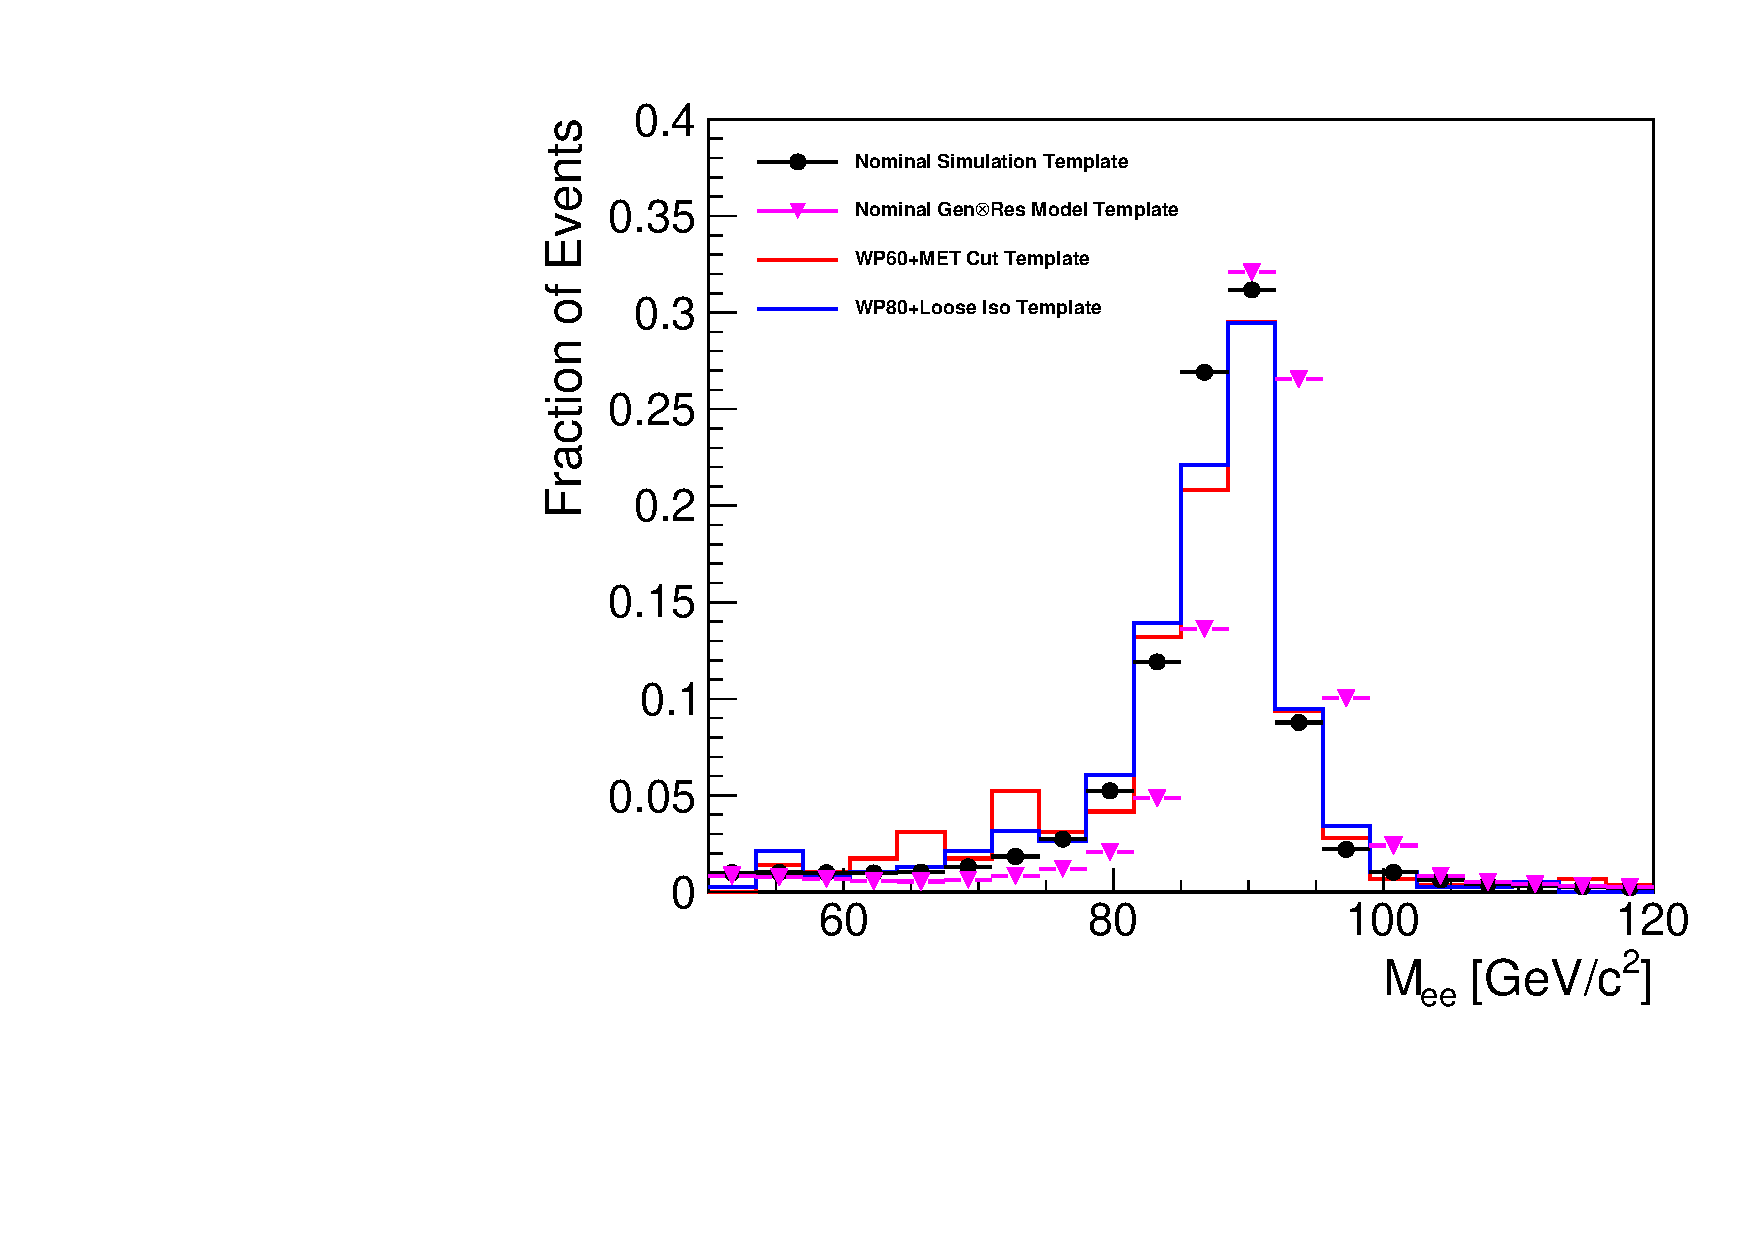
\includegraphics[width=0.49\textwidth]{DataSignalTemplate_Comparison.pdf}%}     
    \caption{Comparison of nominal signal mass shape template from generator-level convolved with resolution 
    model (solid triangles) and from simulation (solid circles) to 
    templates extracted directly from data. We use two data-driven templates to estimate systematic 
     uncertainty in efficiency. In one case (histogram in red color) we select events with \textit{tag} 
     electron passing the WP60 electron selection and a \textit{probe} which fails the WP80 selection, 
     and requiring that the missing transverse energy is less than $20.0$ GeV.  
     In the second case (histogram in blue color) we events with \textit{tag} electron passing the 
     WP80 electron selection and a \textit{probe} which passes the WP95 isolation cuts but fails 
     the WP80 selection.}
    \label{fig:DataSignalTemplate_RecoFailWP80}
  \end{center}
\end{figure}
%%%%%%%%%%%
%%\begin{figure}[htb]
%%  \begin{center}
%%    %\subfigure[]{
%%    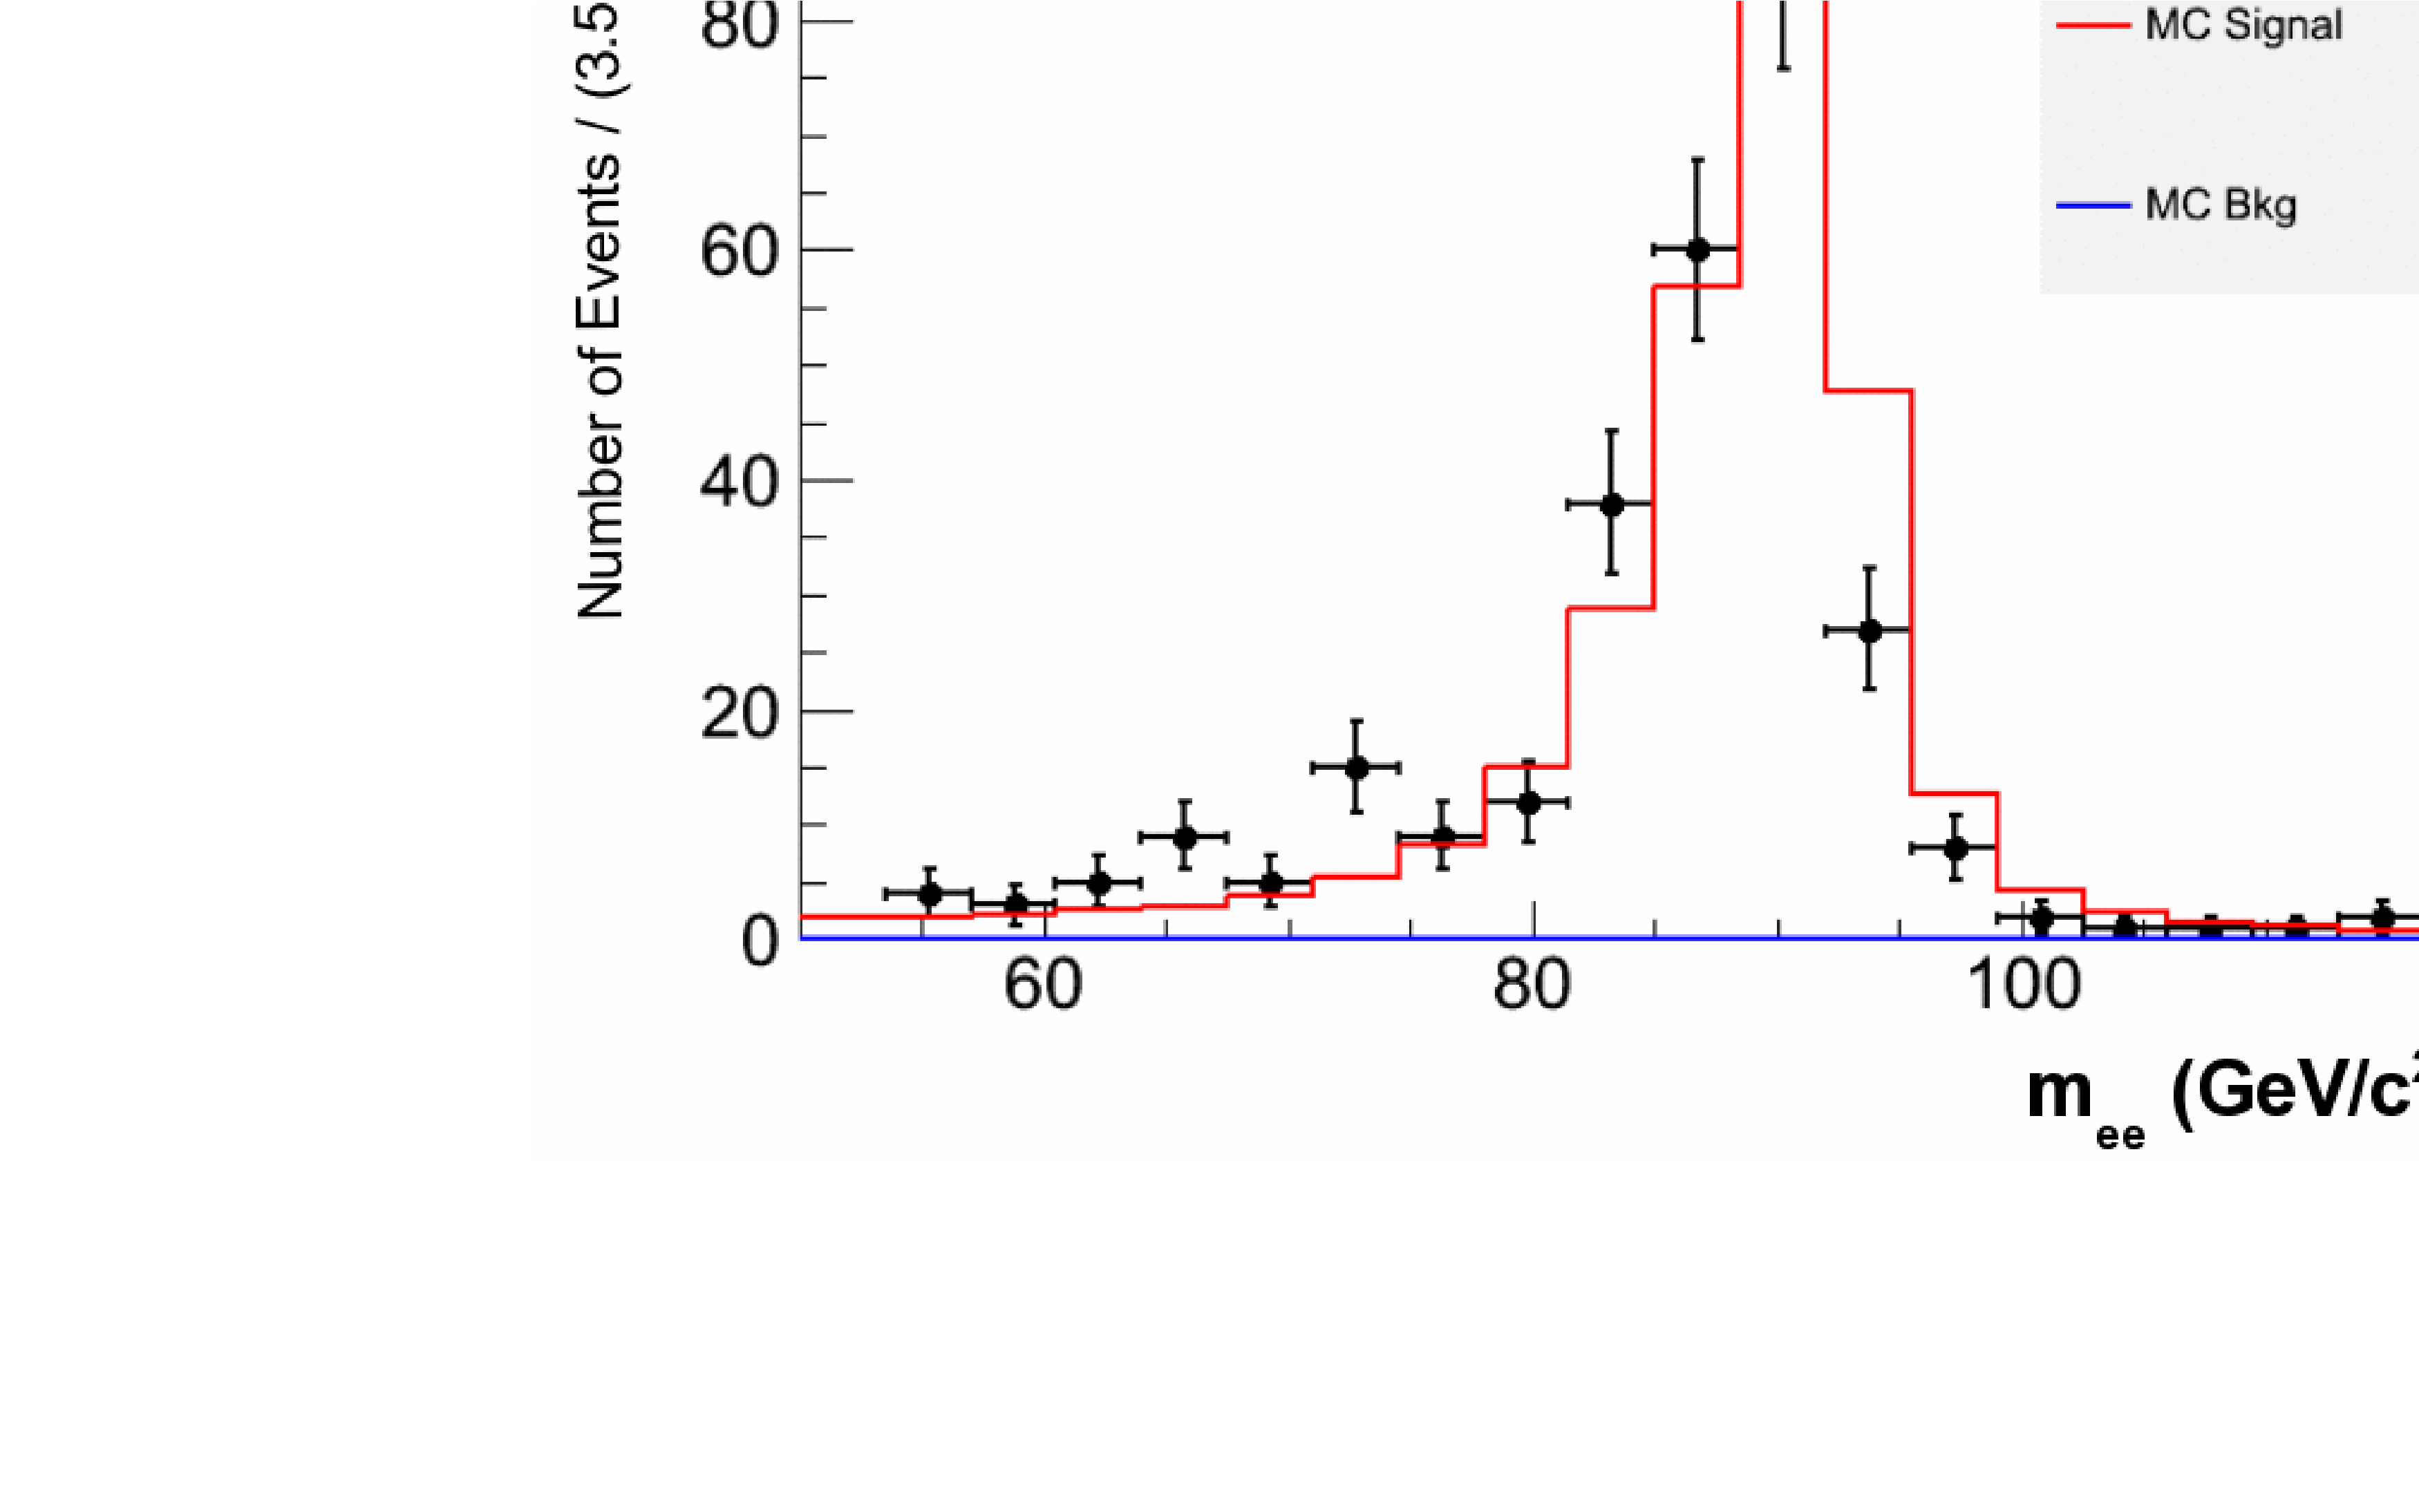
\includegraphics[width=0.49\textwidth]{DataSignalTemplate_RecoFailWP80_Tag60MetCut.pdf}%}     
%%    \caption{Signal mass shape template extracted from data by selecting events with 1 
%%     electron passing the WP60 electron selection and a probe which fails the WP80 selection, 
%%     and requiring that the missing transverse energy is less than $20.0$ GeV. }
%%    \label{fig:DataSignalTemplate_RecoFailWP80_Tag60MetCut}
%%  \end{center}
%%\end{figure}
%%\begin{figure}[htb]
%%  \begin{center}
%%    %\subfigure[]{
%%    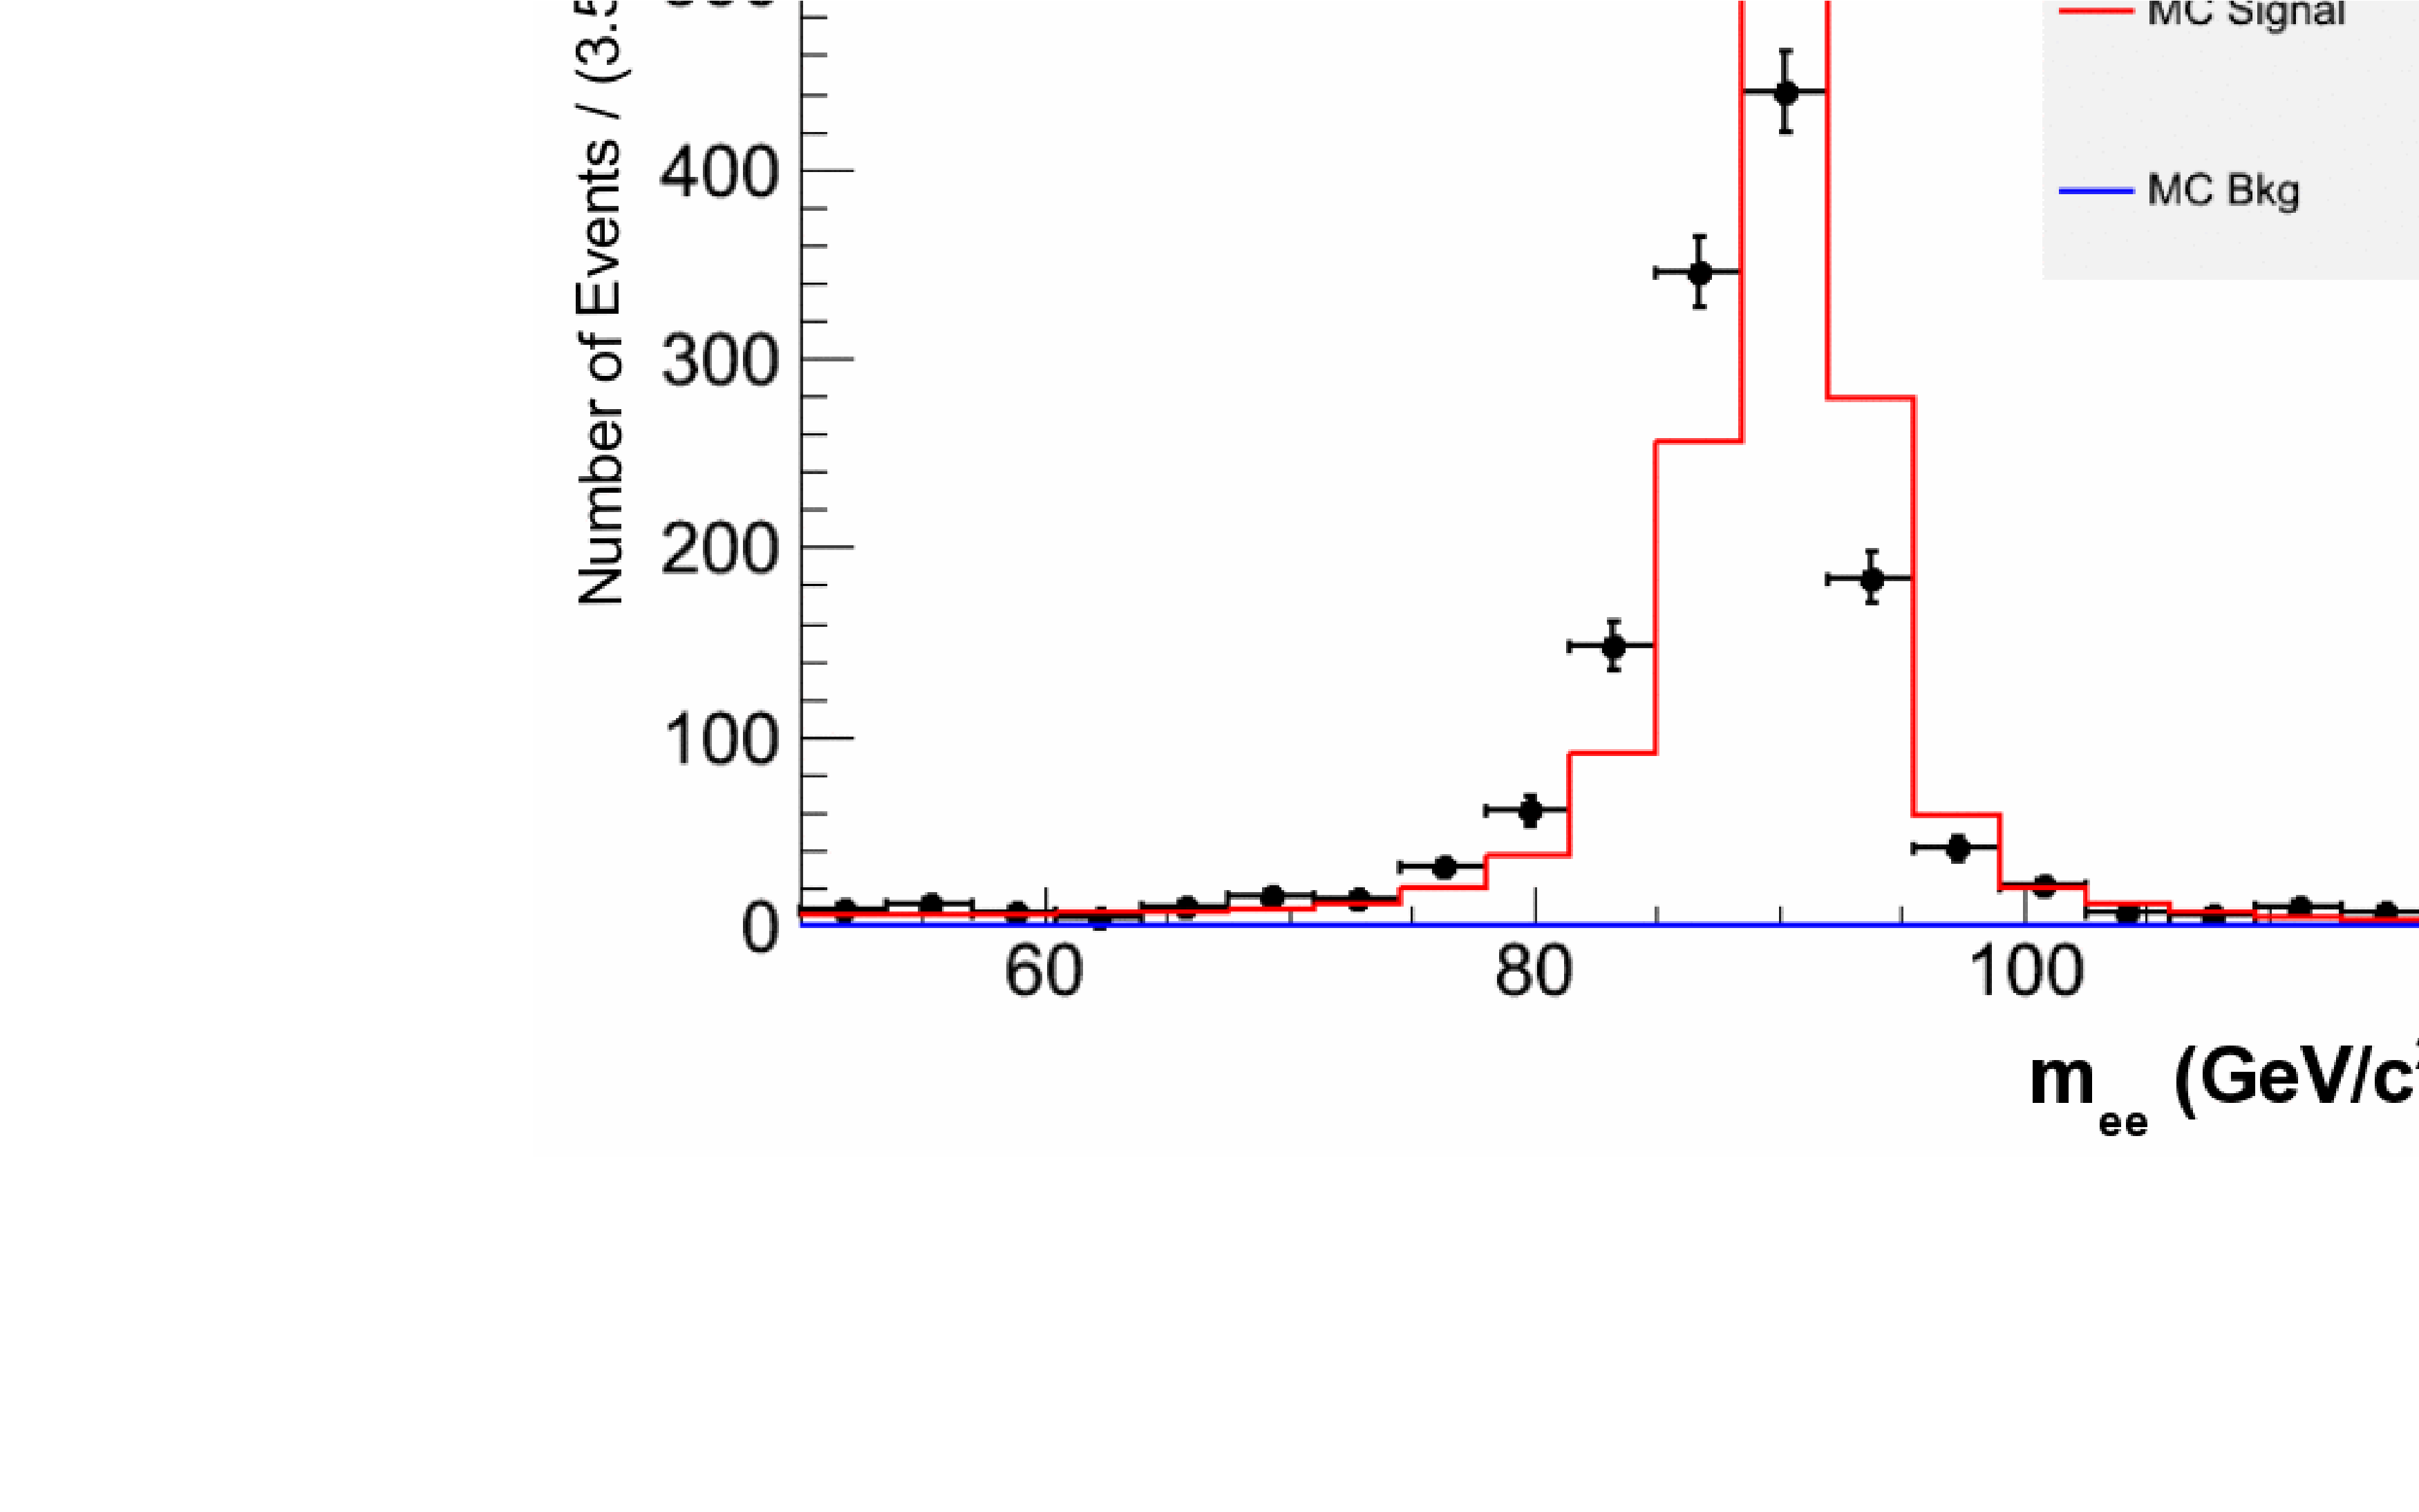
\includegraphics[width=0.49\textwidth]{DataSignalTemplate_RecoFailWP80_Tag80IsoProbe.pdf}%}     
%%    \caption{Signal mass shape template extracted from data by selecting events with 1 
%%     electron passing the WP80 electron selection and a probe which passes the 
%%     WP95 isolation cuts but fails the WP80 selection.}
%%    \label{fig:DataSignalTemplate_RecoFailWP80_Tag80IsoProbe}
%%  \end{center}
%%\end{figure}
To extract systematic uncertainties due to the signal shape, we perform the efficiency fit using these two fixed templates for the signal shape
of the failing sample. The difference between the resulting efficiency measurement and the efficiency measured using the nominal method is taken as a systematic uncertainty. The results of this fit are shown in Figure \ref{fig:Efficiency_RecoToVBTF80_Fail_Systematics_Tag60MetCut} and \ref{fig:Efficiency_RecoToVBTF80_Fail_Systematics_Tag80IsoProbe} for the first and second template respectively. Table \ref{tab:SignalShapeSystematics} summarizes the systematic uncertainties from this procedure. The systematic uncertainties in the endcap are artificially small due to the lack of any events in the mass sidebands in the Tag+Fail sample from tag and probe selection, simply due to the small sample size. A conservative systematic uncertainty of $2\%$ is assigned to both the barrel and the endcap.

\begin{figure}[htb]
  \begin{center}
    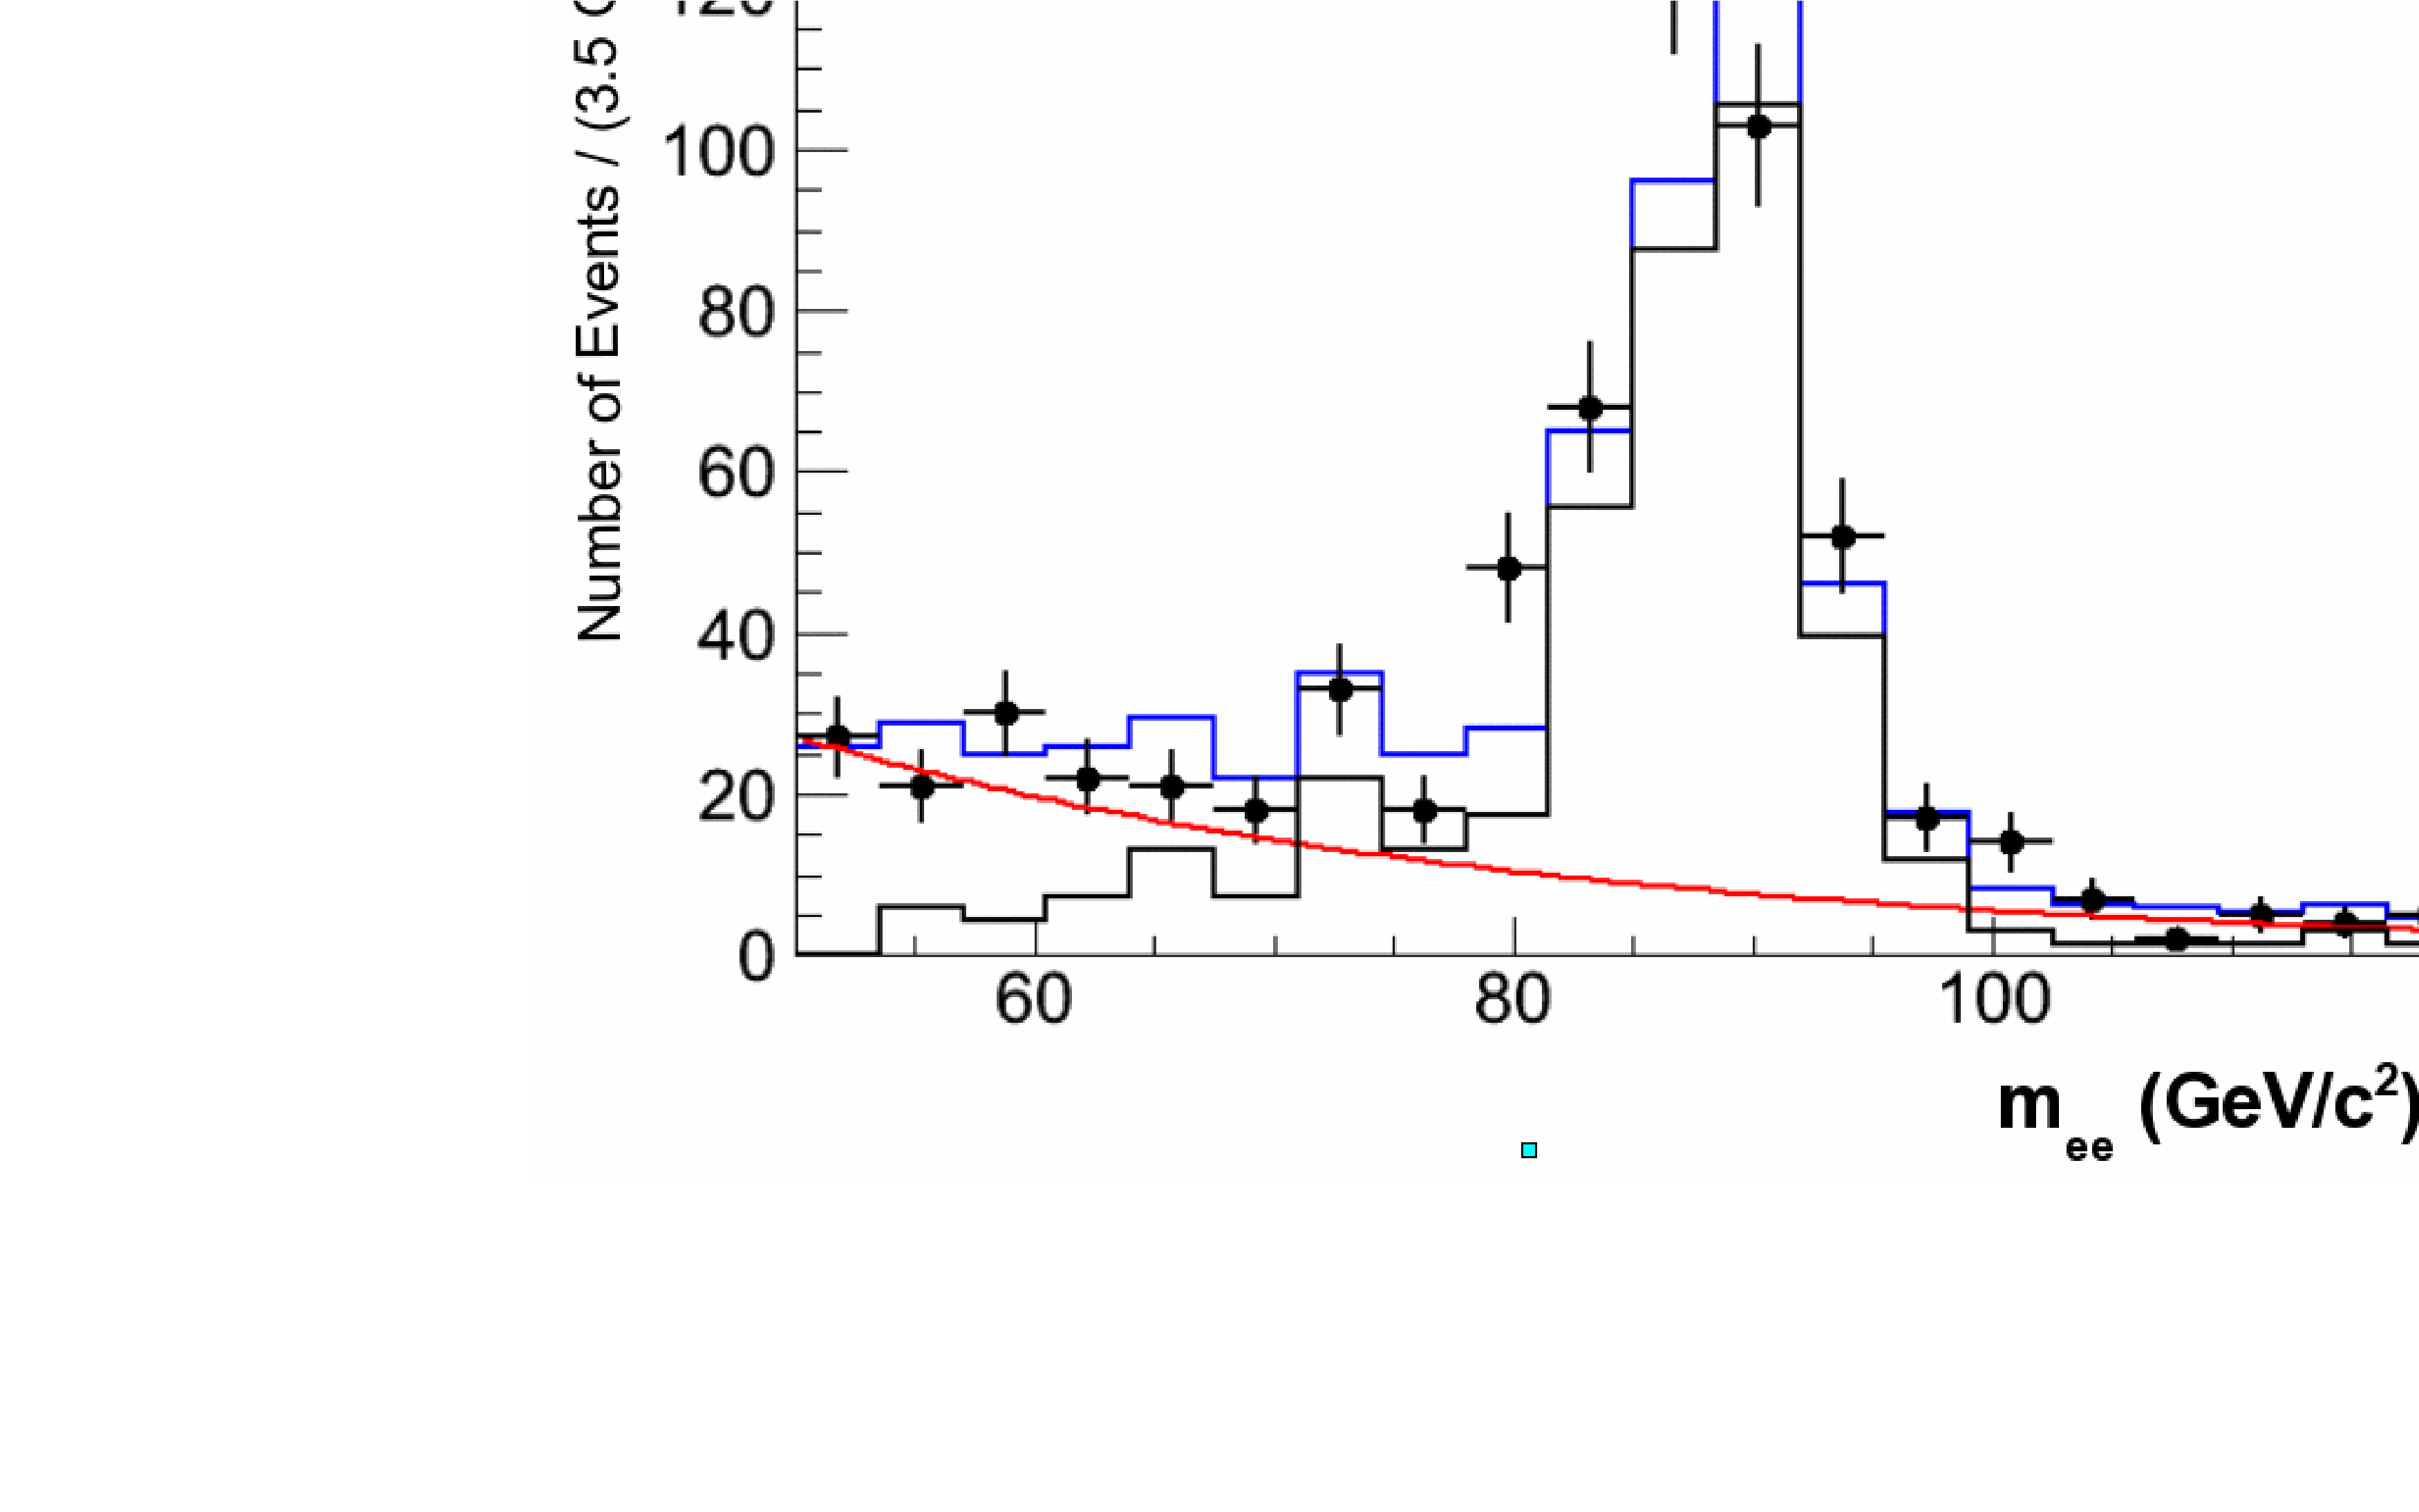
\includegraphics[width=0.49\textwidth]{Efficiency_RecoToVBTF80_Fail_Systematics_Tag60MetCut.pdf}     
    \caption{Fit result for the Tag+Fail sample, using the signal template constructed from selecting WP60 Tag electrons and requiring a missing transverse energy cut. The red curve indicated the fitted background, the black histogram is the fitted signal, and the blue histogram is the fit result for the signal plus background. }
    \label{fig:Efficiency_RecoToVBTF80_Fail_Systematics_Tag60MetCut}
  \end{center}
\end{figure}

\begin{figure}[htb]
  \begin{center}
    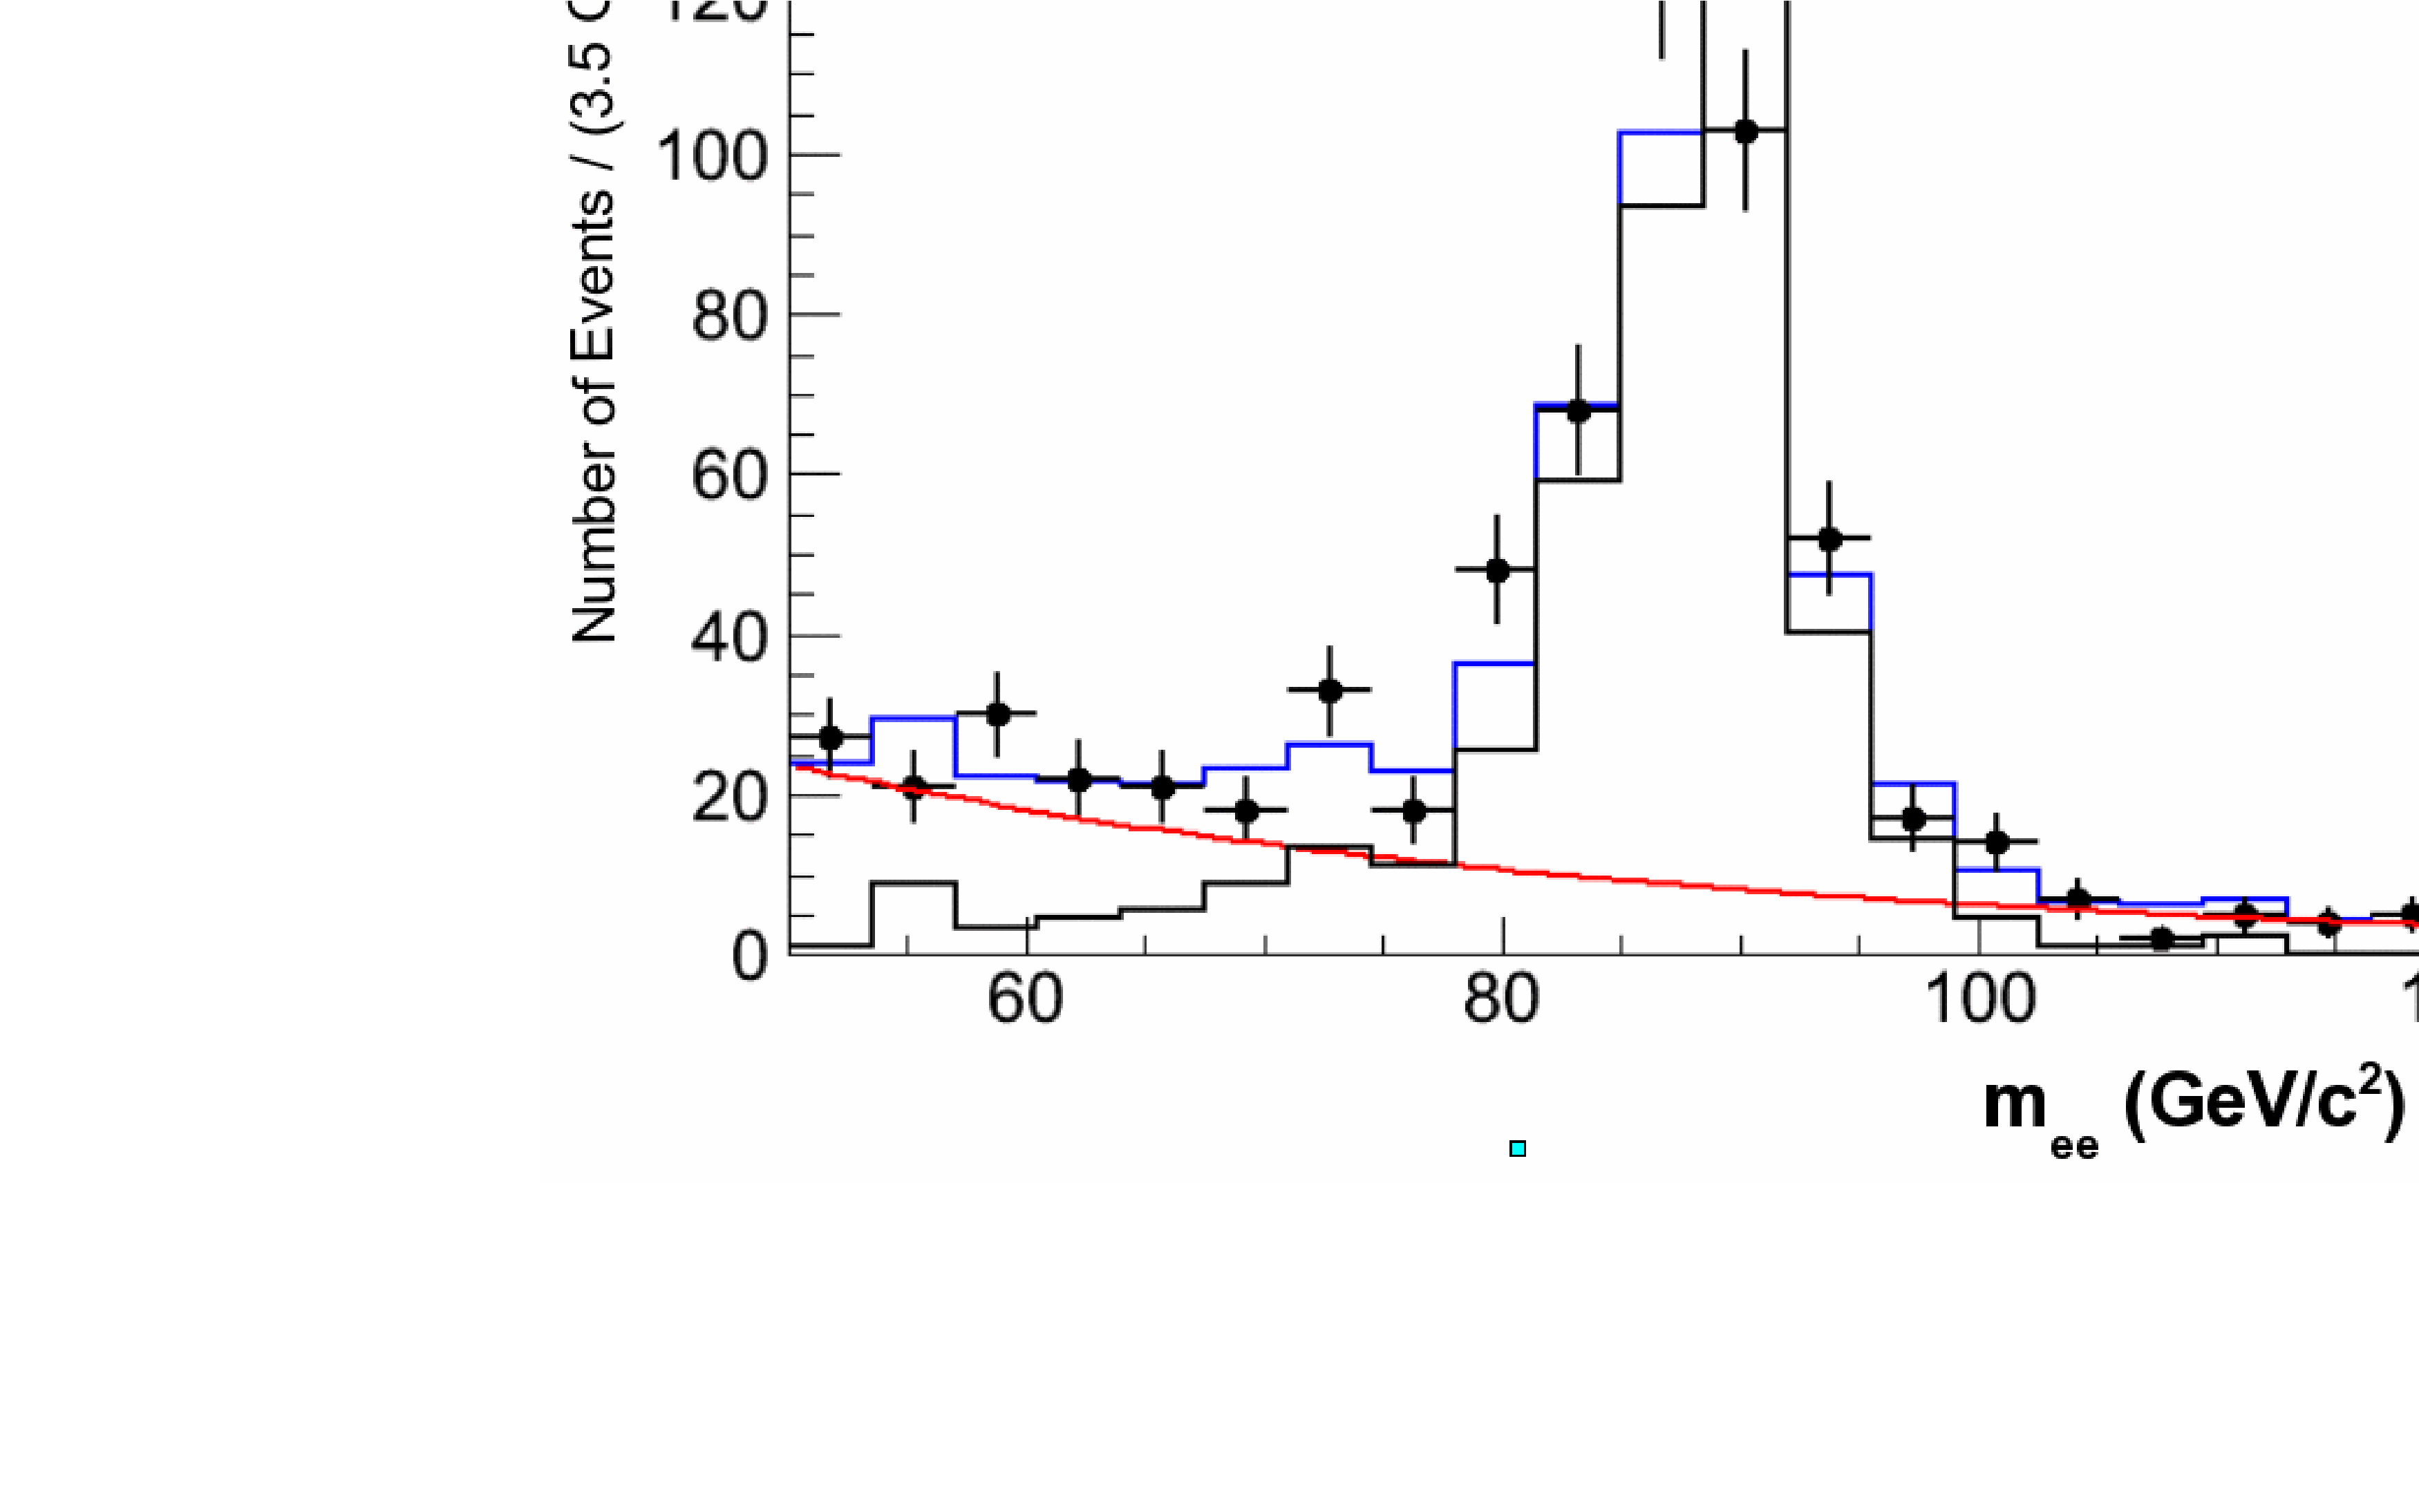
\includegraphics[width=0.49\textwidth]{Efficiency_RecoToVBTF80_Fail_Systematics_Tag80IsoProbe.pdf}     
    \caption{Fit result for the Tag+Fail sample, using the signal template constructed from selecting WP80 Tag electrons and requiring that the probe passes the WP95 isolation cuts. The red curve indicated the fitted background, the black histogram is the fitted signal, and the blue histogram is the fit result for the signal plus background.}
    \label{fig:Efficiency_RecoToVBTF80_Fail_Systematics_Tag80IsoProbe}
  \end{center}
\end{figure}

\begin{table}[!ht]
\begin{center}
\begin{tabular}{c|c|c} \hline \hline
 Data Based Signal Template   &  Barrel  & Endcap  \\ \hline
 WP60 Tag + MetCut            &  1.8\%   & 0.0\%   \\ 
 WP80 Tag + Isolated Probe    &  1.0\%   & 0.2\%   \\ \hline
\end{tabular}
\caption{Systematic uncertainties obtained from the difference between the efficiency measurement using the data driven signal shape templates and the efficiency measured using the nominal signal shape model.\label{tab:SignalShapeSystematics}}
\end{center}
\end{table}


\subsection{Background Shape Systematics}

To estimate the systematic due to the background parametrization, large numbers of pseudo-experiments are generated with a background PDF of the form 1/M$^{\alpha}$, 
where $\alpha=5$.  For each pseudoexperiment S/B is  fixed to the level reported back by the fit to the data for each efficiency step.
This pseudo Monte-Carlo is then fit back to the sum of the signal shape from whence it was generated and several background shape hypothesis, including an exponential decay,
and a power law. 
The systematic uncertainty is then quoted as the maximal difference among the remaining background hypotheses.  The background systematics are found to be small, and
are listed for each efficiency step in table \ref{tab:bkgSyst}. 


\begin{table}
  \begin{center}
    \caption{The Background Parametrization Systematic Uncertainty for each Efficiency Step}
    \label{tab:bkgSyst}
    \vskip 2mm
    \begin{tabular}{c|c}\hline \hline
      Step            & $\Delta\epsilon$ \\ \hline
      SC$\to$Reco     & 0.0006 \\
      Reco$\to$WP80     & 0.002 \\
      WP80$\to$HLT     & 0.0000 \\ \hline
    \end{tabular}
  \end{center}
\end{table}

\subsection{Energy Scale Systematics}
To estimate the systematic due to the uncertainty on the energy scale, the electron energies in the Monte-Carlo are shifted in 
both the positive and negative directions by the uncertainty on the scale.  The maximal difference among the 3 extracted efficiency values
(nominal, positive shift, negative shift) is then taken as the systematic for each step.  The energy scale systematics are found to be quite small, and 
are listed for each efficiency step in table \ref{tab:scaleSyst}.

\begin{table}
  \begin{center}
    \caption{The Energy Scale Systematic Uncertainty for each Efficiency Step}
    \label{tab:scaleSyst}
    \vskip 2mm
    \begin{tabular}{c|c}\hline \hline
      Step            & $\Delta\epsilon$ \\ \hline
      SC$\to$Reco     & 0.001 \\
      Reco$\to$WP80     & 0.002 \\
      WP80$\to$HLT     & 0.001 \\ \hline
    \end{tabular}
  \end{center}
\end{table}



\clearpage

\subsection{Results}
In this section we provide the efficiency results using the generator-level line shape described in Section \ref{sec:genShape}.
These results are summarized in Tables \ref{tab:scRecoResults} - \ref{tab:wp80HltResults}, including all statistical and systematic uncertainties.  The corresponding fit plots are provided in Appendix \ref{genShapePlots}. Results from the Monte-Carlo are also provided, and these were evaluated via simple cut-and-count on the Monte-Carlo truth. For comparison and cross check the results using the alternative simulation based signal shape model are summarized in Appendix \ref{SimulatiobSignalShapeFitPlots}. The 2 approaches yield efficiencies that are in agreement to within the uncertainties. 







%version below uses older stat errors -- uses sqrt(2) factor instead of better sqrt(2-eff) factor
\begin{table}
  \begin{center}
    \caption{The SC$\to$Reco Efficiencies}
    \label{tab:scRecoResults}
    \vskip 2mm
    \begin{minipage}{15cm}
    \begin{tabular}{c|cc|cccc|c}\hline \hline
      Topology &   \multicolumn{2}{c|}{Monte-Carlo} & \multicolumn{4}{c|}{Data} & Data/Monte-Carlo \\ \hline
               &   $\epsilon$ &  $\Delta\epsilon$  & $\epsilon$ & $\Delta\epsilon$ (stat) & $\Delta\epsilon$ (syst) & $\Delta\epsilon$ (total) &   \\ \hline
       EB      &   0.9851     & 0.0002             & 0.986      & 0.005                   & 0.012                   & 0.013                    & 1.001  $\pm$ 0.013 \\ 
       EE      &   0.9629     & 0.0004             & 0.962      & 0.008                   & 0.012                   & 0.015                    & 0.999  $\pm$ 0.016 \\
   EB e$^{-}$  &   0.9854     & 0.0002             & 0.985      & 0.005                   & 0.012                   & 0.013                    & 0.999  $\pm$ 0.013 \\
   EE e$^{-}$  &   0.9624     & 0.0004             & 0.967      & 0.002                   & 0.012                   & 0.012                    & 1.005  $\pm$ 0.012 \\
   EB e$^{+}$  &   0.9849     & 0.0002             & 0.987 \footnote[1]{
                                                                         A minor error was discovered for this fit in that the exponentially falling background shape flipped
									 to instead be growing in the Tag+Fail sample.  The fit was later constrained to prevent this and yielded the corrected result:
									 $\epsilon$ = 0.989 $\pm$ 0.006 (stat).  As the difference is negligible, the original result quoted in the table above has been 
									 retained throughout the analysis, though the corresponding plots in Figure \ref{fig:scRecoEbPlus}
									 have been updated to the corrected fit.}
                                                                & 0.004                   & 0.012                   & 0.013                    & 1.002  $\pm$ 0.012 \\
   EE e$^{+}$  &   0.9634     & 0.0004             & 0.951      & 0.003                   & 0.012                   & 0.012                    & 0.987  $\pm$ 0.012 \\ \hline
    \end{tabular}
    %\caption[1]{A minor error was discovered for this fit in that the exponentially falling background shape flipped to instead be growing.  The fit was
    %later constrained to prevent this and yielded the corrected result:  $\epsilon$ = 0.989 $\pm$ 0.006.  As the difference is quite negligable, the original result has
    %been retained for the analysis, though the corresponding plots \ref{fig:scRecoEbPlus} in \ref{genShapePlots} have been updated to the corrected fit.}
    \end{minipage}
  \end{center}
\end{table}
\begin{table}
  \begin{center}
    \caption{The Reco$\to$WP80 Efficiencies}
    \label{tab:recoWP80Results}
    \vskip 2mm
    \begin{tabular}{c|cc|cccc|c}\hline \hline
      Topology &   \multicolumn{2}{c|}{Monte-Carlo} & \multicolumn{4}{c|}{Data} & Data/Monte-Carlo \\ \hline
               &   $\epsilon$ &  $\Delta\epsilon$  & $\epsilon$ & $\Delta\epsilon$ (stat) & $\Delta\epsilon$ (syst) & $\Delta\epsilon$ (total) &   \\ \hline
      EB       &   0.8547     & 0.0004             & 0.791      & 0.018                   & 0.020                   & 0.027                    & 0.925 $\pm$ 0.032 \\ 
      EE       &   0.7488     & 0.0006             & 0.692      & 0.020                   & 0.020                   & 0.028                    & 0.924 $\pm$ 0.037 \\
   EB e$^{-}$  &   0.8545     & 0.0005             & 0.793      & 0.027                   & 0.020                   & 0.034                    & 0.929 $\pm$ 0.040 \\
   EE e$^{-}$  &   0.7489     & 0.0009             & 0.701      & 0.038                   & 0.020                   & 0.043                    & 0.936 $\pm$ 0.057 \\
   EB e$^{+}$  &   0.8549     & 0.0005             & 0.780      & 0.031                   & 0.020                   & 0.037                    & 0.913 $\pm$ 0.044 \\
   EE e$^{+}$  &   0.7487     & 0.0009             & 0.701      & 0.029                   & 0.020                   & 0.035                    & 0.936 $\pm$ 0.047 \\ \hline
    \end{tabular}
  \end{center}
\end{table}
\begin{table}
  \begin{center}
    \caption{The WP80$\to$HLT Efficiencies}
    \label{tab:wp80HltResults}
    \vskip 2mm
    \begin{tabular}{c|cc|cccc|c}\hline \hline
      Topology &   \multicolumn{2}{c|}{Monte-Carlo} & \multicolumn{4}{c|}{Data} & Data/Monte-Carlo  \\ \hline
               &   $\epsilon$ &  $\Delta\epsilon$  & $\epsilon$ & $\Delta\epsilon$ (stat) & $\Delta\epsilon$ (syst) & $\Delta\epsilon$ (total) &  \\ \hline
      EB       &   0.997     & 0.0001             & 0.989     & 0.003                  & 0.001                  & 0.0032                   & 0.992 $\pm$ 0.003 \\
      EE       &   0.988     & 0.0003             & 0.992     & 0.005                  & 0.001                  & 0.0051                   & 1.004 $\pm$ 0.005 \\
   EB e$^{-}$  &   0.997     & 0.0001             & 0.986     & 0.005                  & 0.001                  & 0.0051                   & 0.989 $\pm$ 0.005 \\
   EE e$^{-}$  &   0.988     & 0.0004             & 0.994     & 0.006                  & 0.001                  & 0.0061                   & 1.006 $\pm$ 0.006 \\
   EB e$^{+}$  &   0.996     & 0.0001             & 0.994     & 0.004                  & 0.001                  & 0.0042                   & 0.998 $\pm$ 0.004 \\
   EE e$^{+}$  &   0.989     & 0.0004             & 0.990     & 0.007                  & 0.001                  & 0.0071                   & 1.001 $\pm$ 0.007 \\ \hline
    \end{tabular}
  \end{center}
\end{table}



%version below uses better stat errors -- uses sqrt(2 - eff) factor instead of older just sqrt(2) factor
%\begin{table}
%  \begin{center}
%    \caption{The SC$\to$Reco Efficiencies}
%    \label{tab:scRecoResults}
%    \vskip 2mm
%    \begin{tabular}{c|cc|cccc|c}\hline \hline
%      Topology &   \multicolumn{2}{c|}{Monte-Carlo} & \multicolumn{4}{c|}{Data} & Data/Monte-Carlo \\ \hline
%               &   $\epsilon$ &  $\Delta\epsilon$  & $\epsilon$ & $\Delta\epsilon$ (stat) & $\Delta\epsilon$ (syst) & $\Delta\epsilon$ (total) &   \\ \hline
%       EB      &   0.9851     & 0.0002             & 0.986      & 0.004                   & 0.012                   & 0.013                    & 1.001  $\pm$ 0.013 \\ 
%       EE      &   0.9629     & 0.0004             & 0.962      & 0.006                   & 0.012                   & 0.013                    & 0.999  $\pm$ 0.012 \\
%   EB e$^{-}$  &   0.9854     & 0.0002             & 0.985      & 0.003                   & 0.012                   & 0.012                    & 0.999  $\pm$ 0.012 \\
%   EE e$^{-}$  &   0.9624     & 0.0004             & 0.967      & 0.002                   & 0.012                   & 0.012                    & 1.005  $\pm$ 0.012 \\
%   EB e$^{+}$  &   0.9849     & 0.0002             & 0.987      & 0.003                   & 0.012                   & 0.012                    & 1.002  $\pm$ 0.012 \\
%   EE e$^{+}$  &   0.9634     & 0.0004             & 0.951      & 0.002                   & 0.012                   & 0.012                    & 0.987  $\pm$ 0.012 \\ \hline
%    \end{tabular}
%  \end{center}
%\end{table}
%\begin{table}
%  \begin{center}
%    \caption{The Reco$\to$WP80 Efficiencies}
%    \label{tab:recoWP80Results}
%    \vskip 2mm
%    \begin{tabular}{c|cc|cccc|c}\hline \hline
%      Topology &   \multicolumn{2}{c|}{Monte-Carlo} & \multicolumn{4}{c|}{Data} & Data/Monte-Carlo \\ \hline
%               &   $\epsilon$ &  $\Delta\epsilon$  & $\epsilon$ & $\Delta\epsilon$ (stat) & $\Delta\epsilon$ (syst) & $\Delta\epsilon$ (total) &   \\ \hline
%      EB       &   0.8547     & 0.0004             & 0.791      & 0.014                   & 0.020                   & 0.024                    & 0.925 $\pm$ 0.028 \\ 
%      EE       &   0.7488     & 0.0006             & 0.692      & 0.016                   & 0.020                   & 0.026                    & 0.924 $\pm$ 0.035 \\
%   EB e$^{-}$  &   0.8545     & 0.0005             & 0.793      & 0.021                   & 0.020                   & 0.029                    & 0.929 $\pm$ 0.034 \\
%   EE e$^{-}$  &   0.7489     & 0.0009             & 0.701      & 0.030                   & 0.020                   & 0.036                    & 0.936 $\pm$ 0.048 \\
%   EB e$^{+}$  &   0.8549     & 0.0005             & 0.780      & 0.024                   & 0.020                   & 0.031                    & 0.913 $\pm$ 0.036 \\
%   EE e$^{+}$  &   0.7487     & 0.0009             & 0.701      & 0.023                   & 0.020                   & 0.030                    & 0.936 $\pm$ 0.040 \\ \hline
%    \end{tabular}
%  \end{center}
%\end{table}
%\begin{table}
%  \begin{center}
%    \caption{The WP80$\to$HLT Efficiencies}
%    \label{tab:wp80HltResults}
%    \vskip 2mm
%    \begin{tabular}{c|cc|cccc|c}\hline \hline
%      Topology &   \multicolumn{2}{c|}{Monte-Carlo} & \multicolumn{4}{c|}{Data} & Data/Monte-Carlo  \\ \hline
%               &   $\epsilon$ &  $\Delta\epsilon$  & $\epsilon$ & $\Delta\epsilon$ (stat) & $\Delta\epsilon$ (syst) & $\Delta\epsilon$ (total) &  \\ \hline
%      EB       &   0.997     & 0.0001             & 0.989     & 0.002                  & 0.001                  & 0.0022                   & 0.992 $\pm$ 0.002 \\
%      EE       &   0.988     & 0.0003             & 0.992     & 0.004                  & 0.001                  & 0.0041                   & 1.004 $\pm$ 0.004 \\
%   EB e$^{-}$  &   0.997     & 0.0001             & 0.986     & 0.004                  & 0.001                  & 0.0041                   & 0.989 $\pm$ 0.004 \\
%   EE e$^{-}$  &   0.988     & 0.0004             & 0.994     & 0.004                  & 0.001                  & 0.0041                   & 1.006 $\pm$ 0.004 \\
%   EB e$^{+}$  &   0.996     & 0.0001             & 0.994     & 0.003                  & 0.001                  & 0.0032                   & 0.998 $\pm$ 0.003 \\
%   EE e$^{+}$  &   0.989     & 0.0004             & 0.990     & 0.005                  & 0.001                  & 0.0051                   & 1.001 $\pm$ 0.005 \\ \hline
%    \end{tabular}
%  \end{center}
%\end{table}

\section{Conclusions}
We have presented the first electron efficiency measurements performed at CMS. These measurements were performed as part of the W and Z inclusive cross section measurements, and used 2.88 pb$^{-1}$ of pp Collision Data at $\sqrt s = 7$ TeV. This note has summarized these measurements, described all of the associated systematic uncertainties.


\newpage
\begin{thebibliography}{10}
\bibitem{CMSAN2010/264}
\textit{Updated Measurements of Inclusive W and Z Cross Sections at 7 TeV}, CMS AN-2010/264.
\bibitem{CMSAN2009/111}
\textit{Generic Tag and Probe Tool for Measuring Efficiency at CMS with Early Data}, CMS AN-2009/111.
%\bibitem{CMSAN2007/019}
%\textit{Measuring Electron Efficiencies at CMS with Early Data}, CMS AN-2007/019.
\bibitem{CMSAN2010/277}
\textit{Data Driven Techniques to Estimate the Background in the Z$\to$ee Events}, CMS AN-2010/277.
\bibitem{CMSAN2010/284}
\textit{Fake Lepton Background Estimate for the Z$\to$ee Cross Section Measurement using the Fake Rate Method}, CMS AN-2010/284.
\bibitem{Powheg}
\textit{A New Method for Combining NLO QCD with Shower Monte Carlo Algorithms},
P. Nason, JHEP 0411, 040 (2004) [arXiv:hep-ph/0409146].
\bibitem{MINOS}
D.Drijard, Statistical Methods in Experimental Physics, North-Holland, 1971.
%\end{thebibliography}

\newpage


\appendix 
\section{Simulation Based Signal Shape Fit Plots}
\label{SimulatiobSignalShapeFitPlots}

%reco->wp80
\begin{figure}[htb]
  \begin{center}
    \subfigure[]{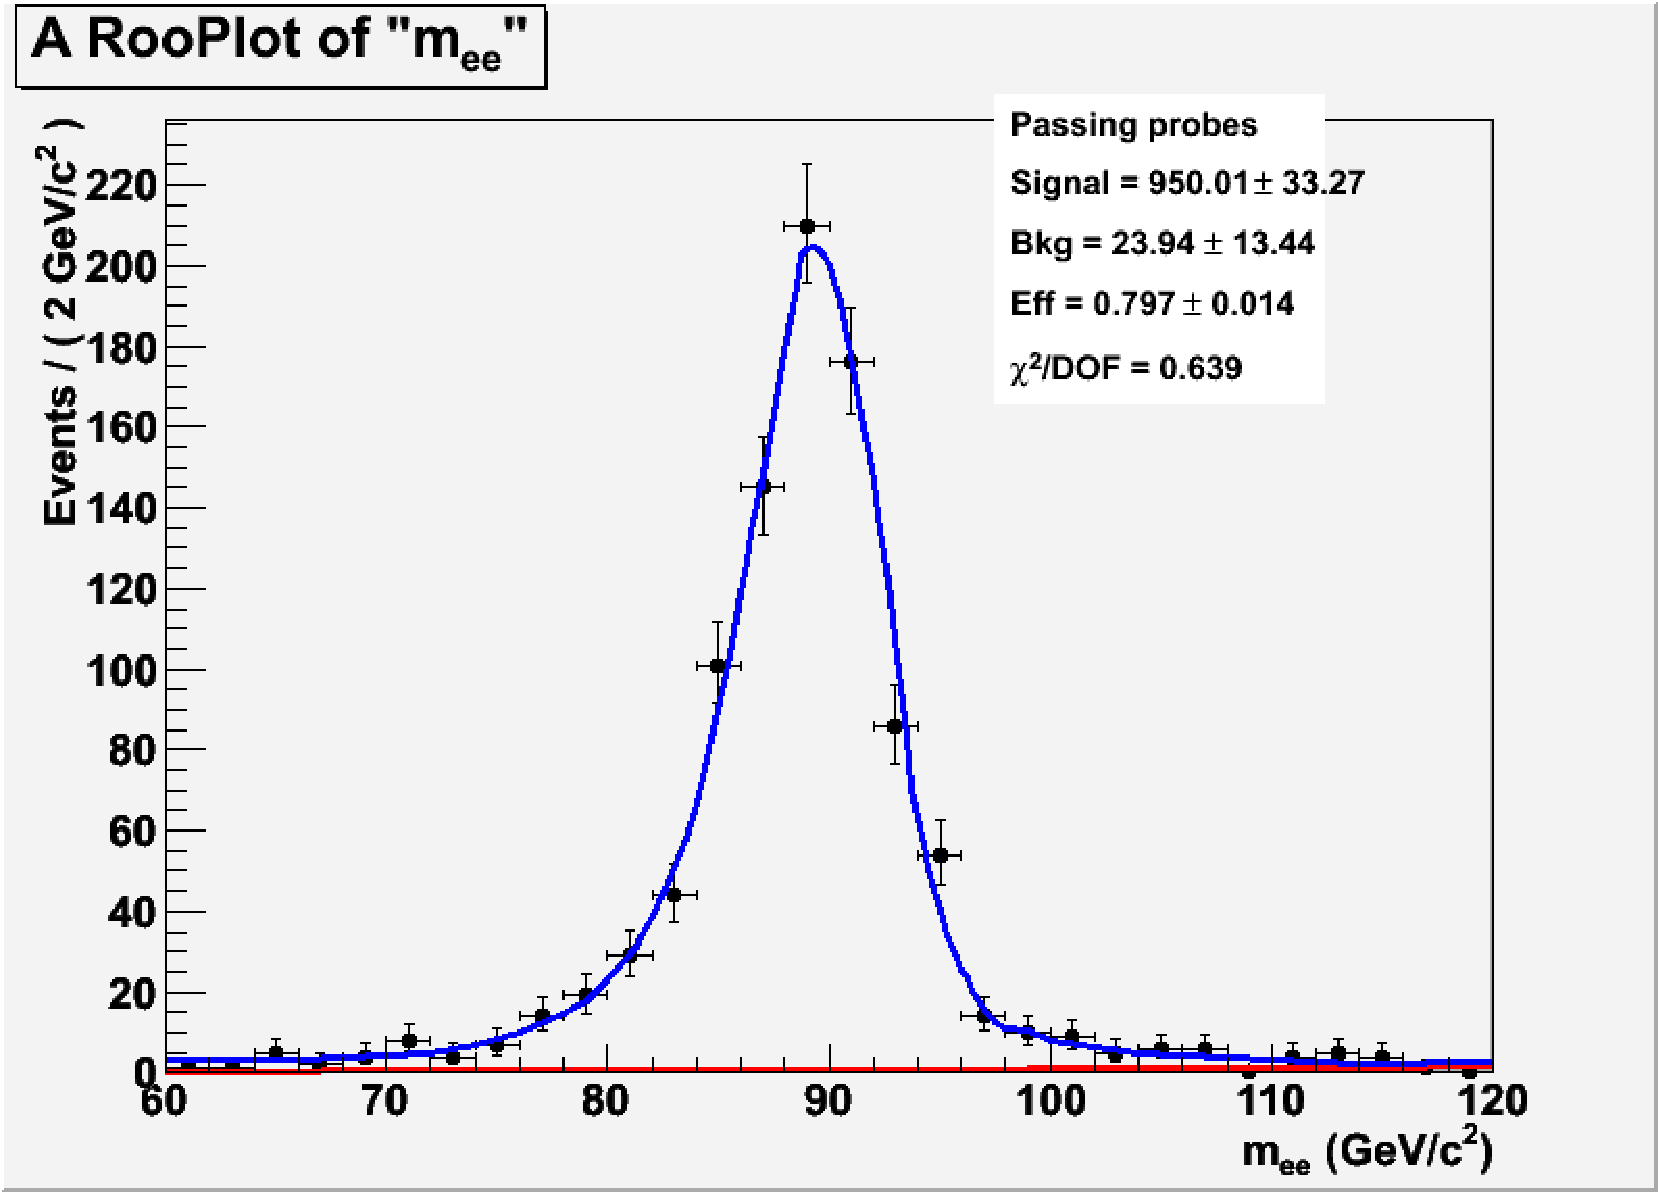
\includegraphics[width=0.49\textwidth]{Efficiency_RecoToVBTF80_MCSignalShape_EB_Pass.pdf}}
    \subfigure[]{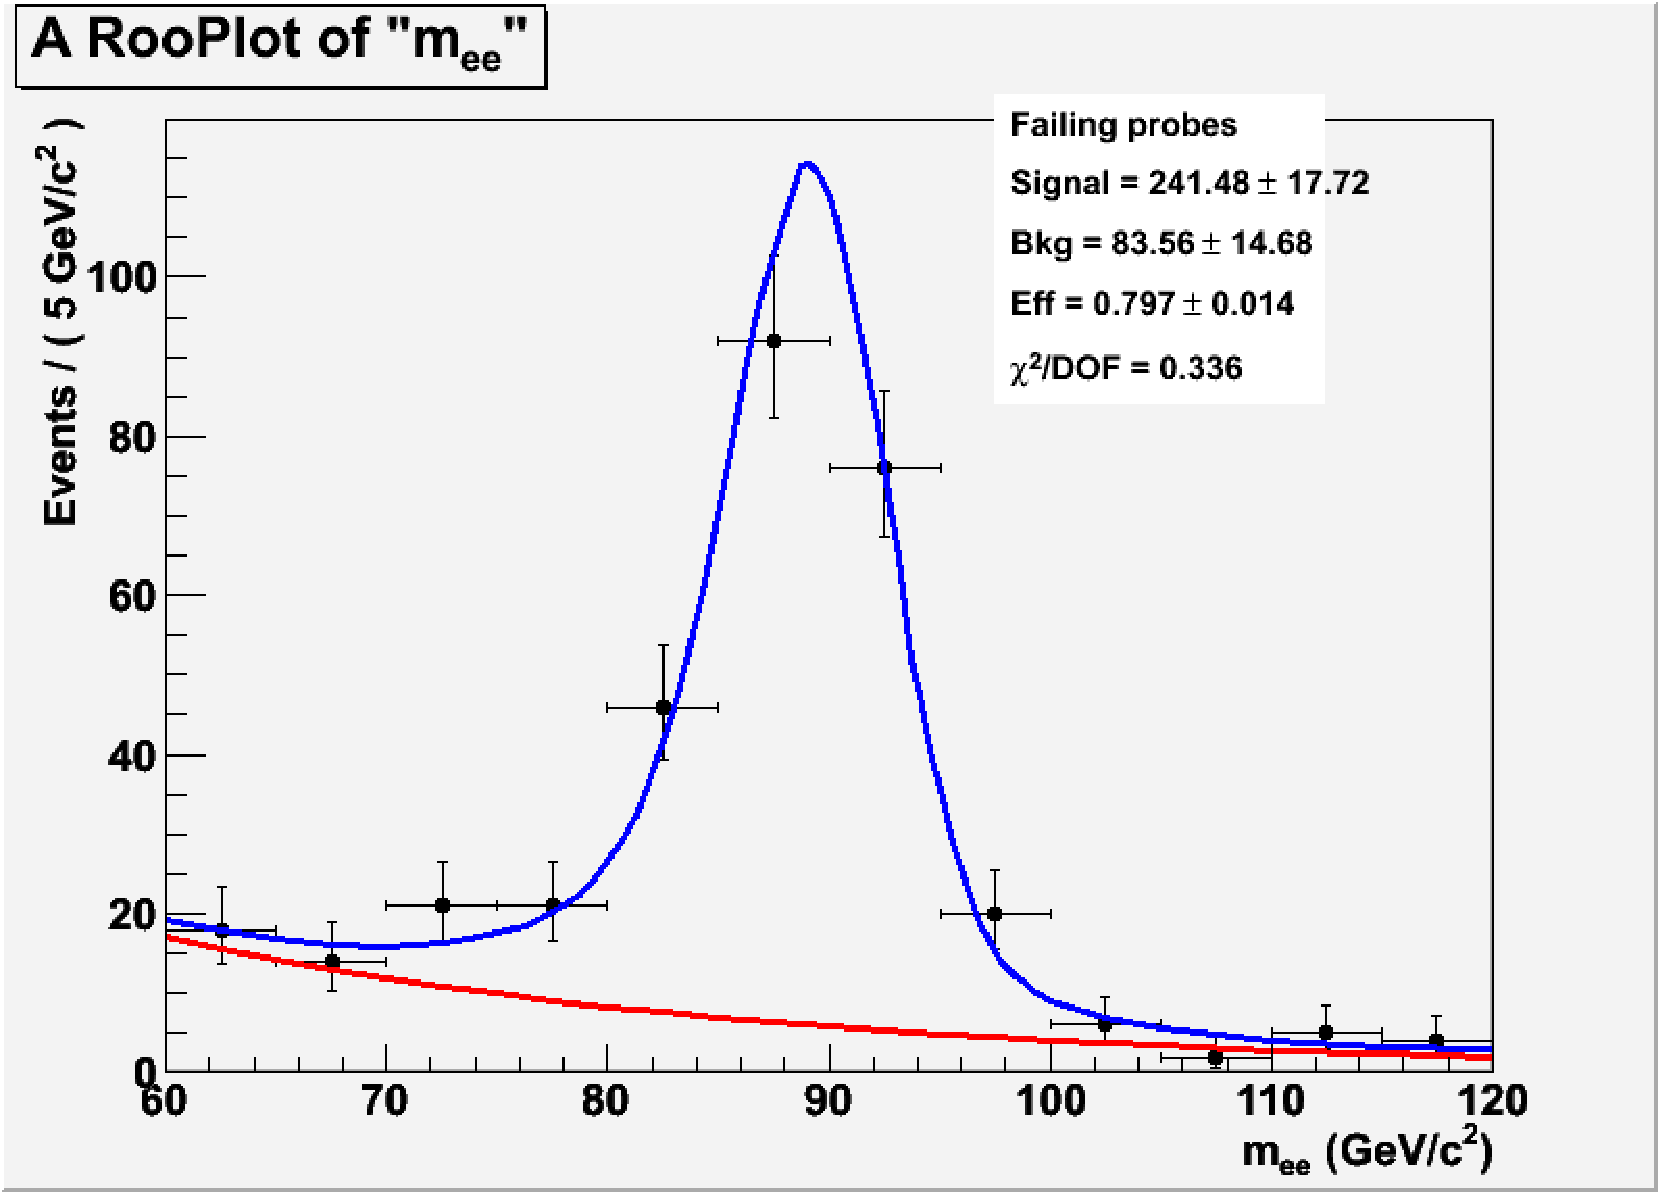
\includegraphics[width=0.49\textwidth]{Efficiency_RecoToVBTF80_MCSignalShape_EB_Fail.pdf}}
    \caption{The passing (a) and failing (b) fits for the Reco$\to$WP80 step in the Ecal Barrel.
             The data is in black, background fit in red, and signal+background fit in blue.}
  \end{center}
\end{figure}

\begin{figure}[htb]
  \begin{center}
    \subfigure[]{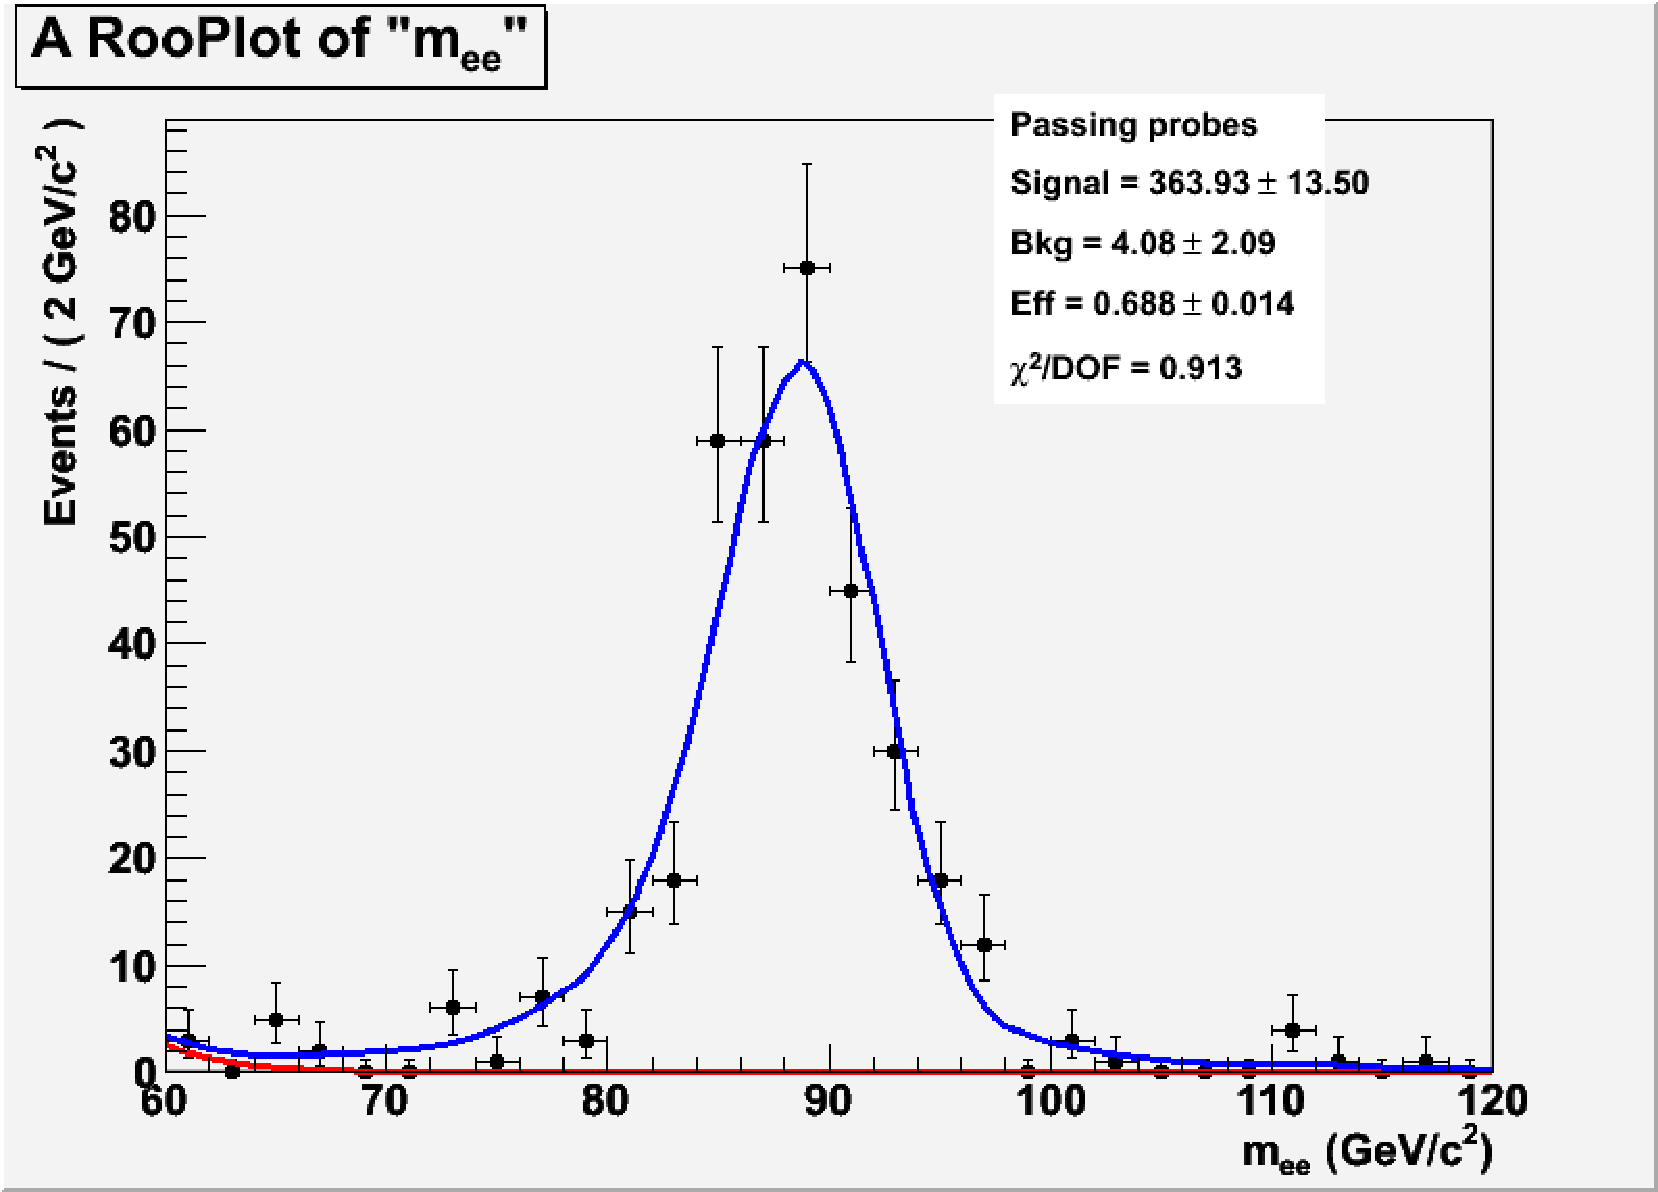
\includegraphics[width=0.49\textwidth]{Efficiency_RecoToVBTF80_MCSignalShape_EE_Pass.pdf}}
    \subfigure[]{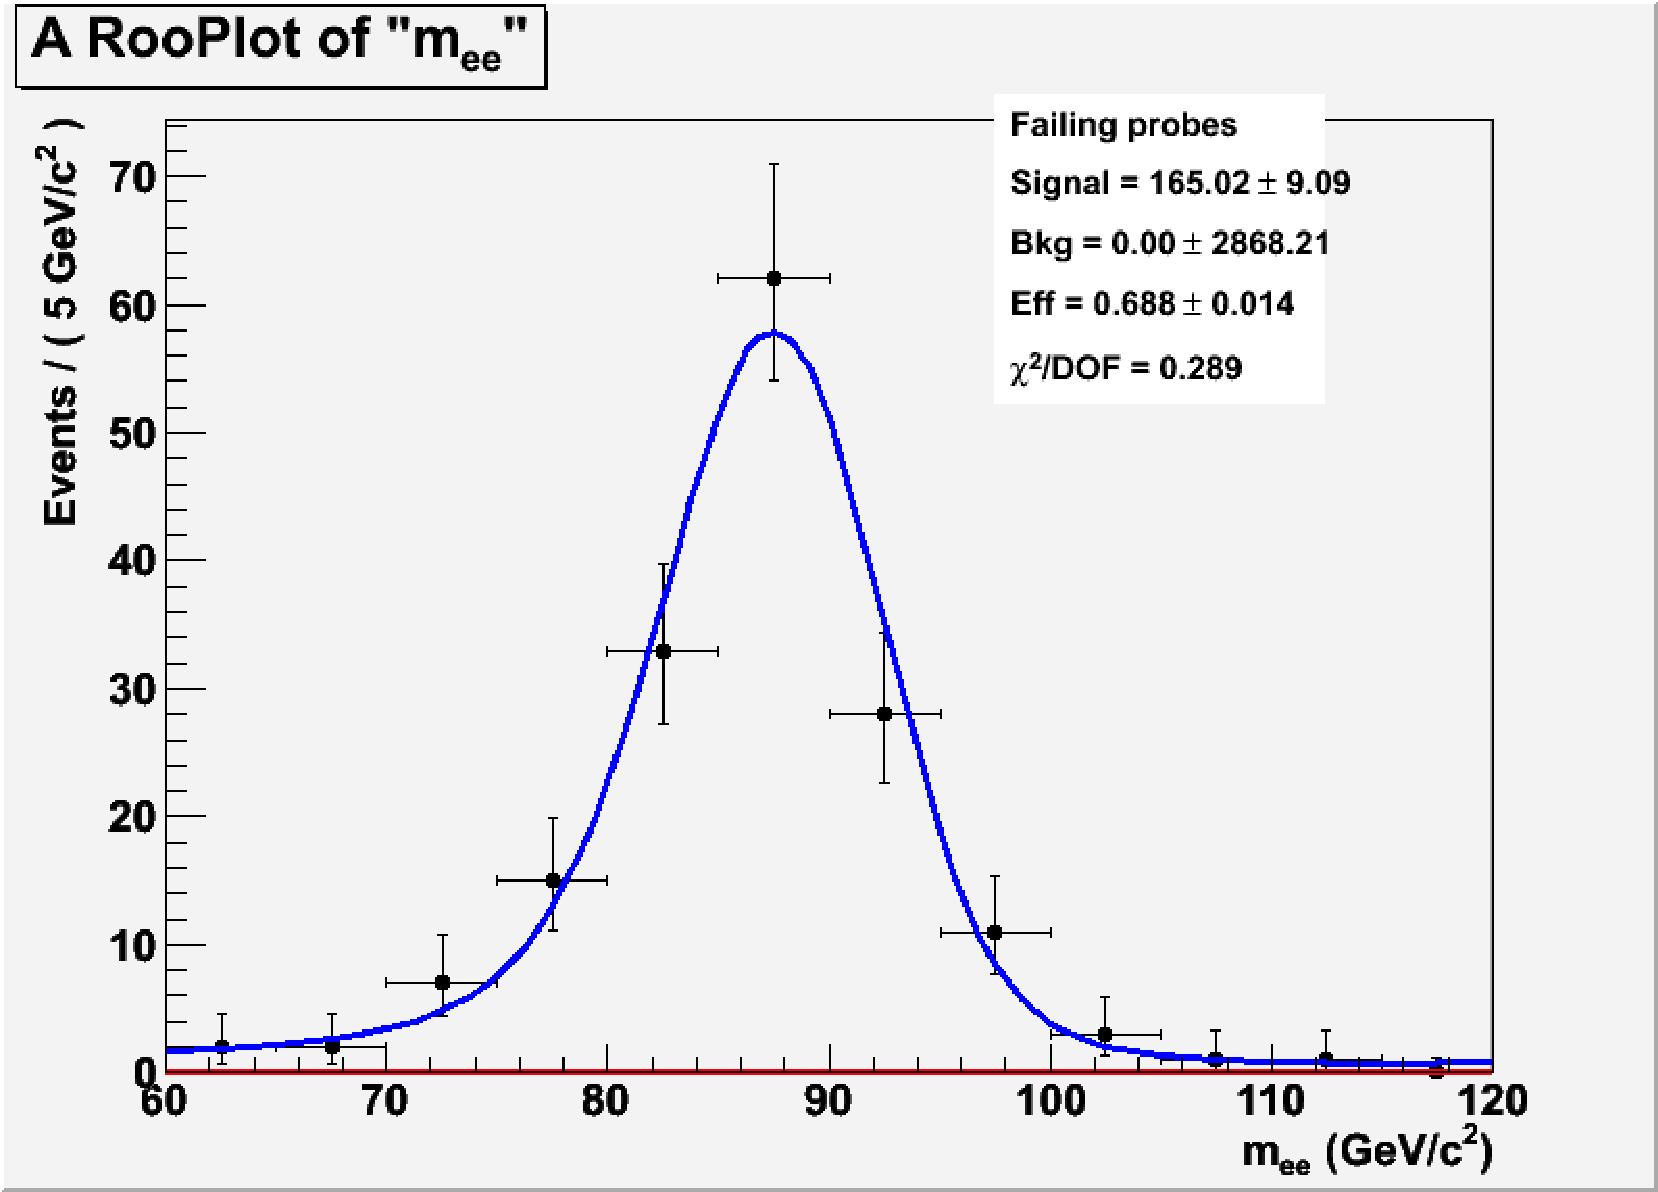
\includegraphics[width=0.49\textwidth]{Efficiency_RecoToVBTF80_MCSignalShape_EE_Fail.pdf}}
    \caption{The passing (a) and failing (b) fits for the Reco$\to$WP80 step in the Ecal Endcap.  
             The data is in black, background fit in red, and signal+background fit in blue.}
  \end{center}
\end{figure}

\begin{figure}[htb]
  \begin{center}
    \subfigure[]{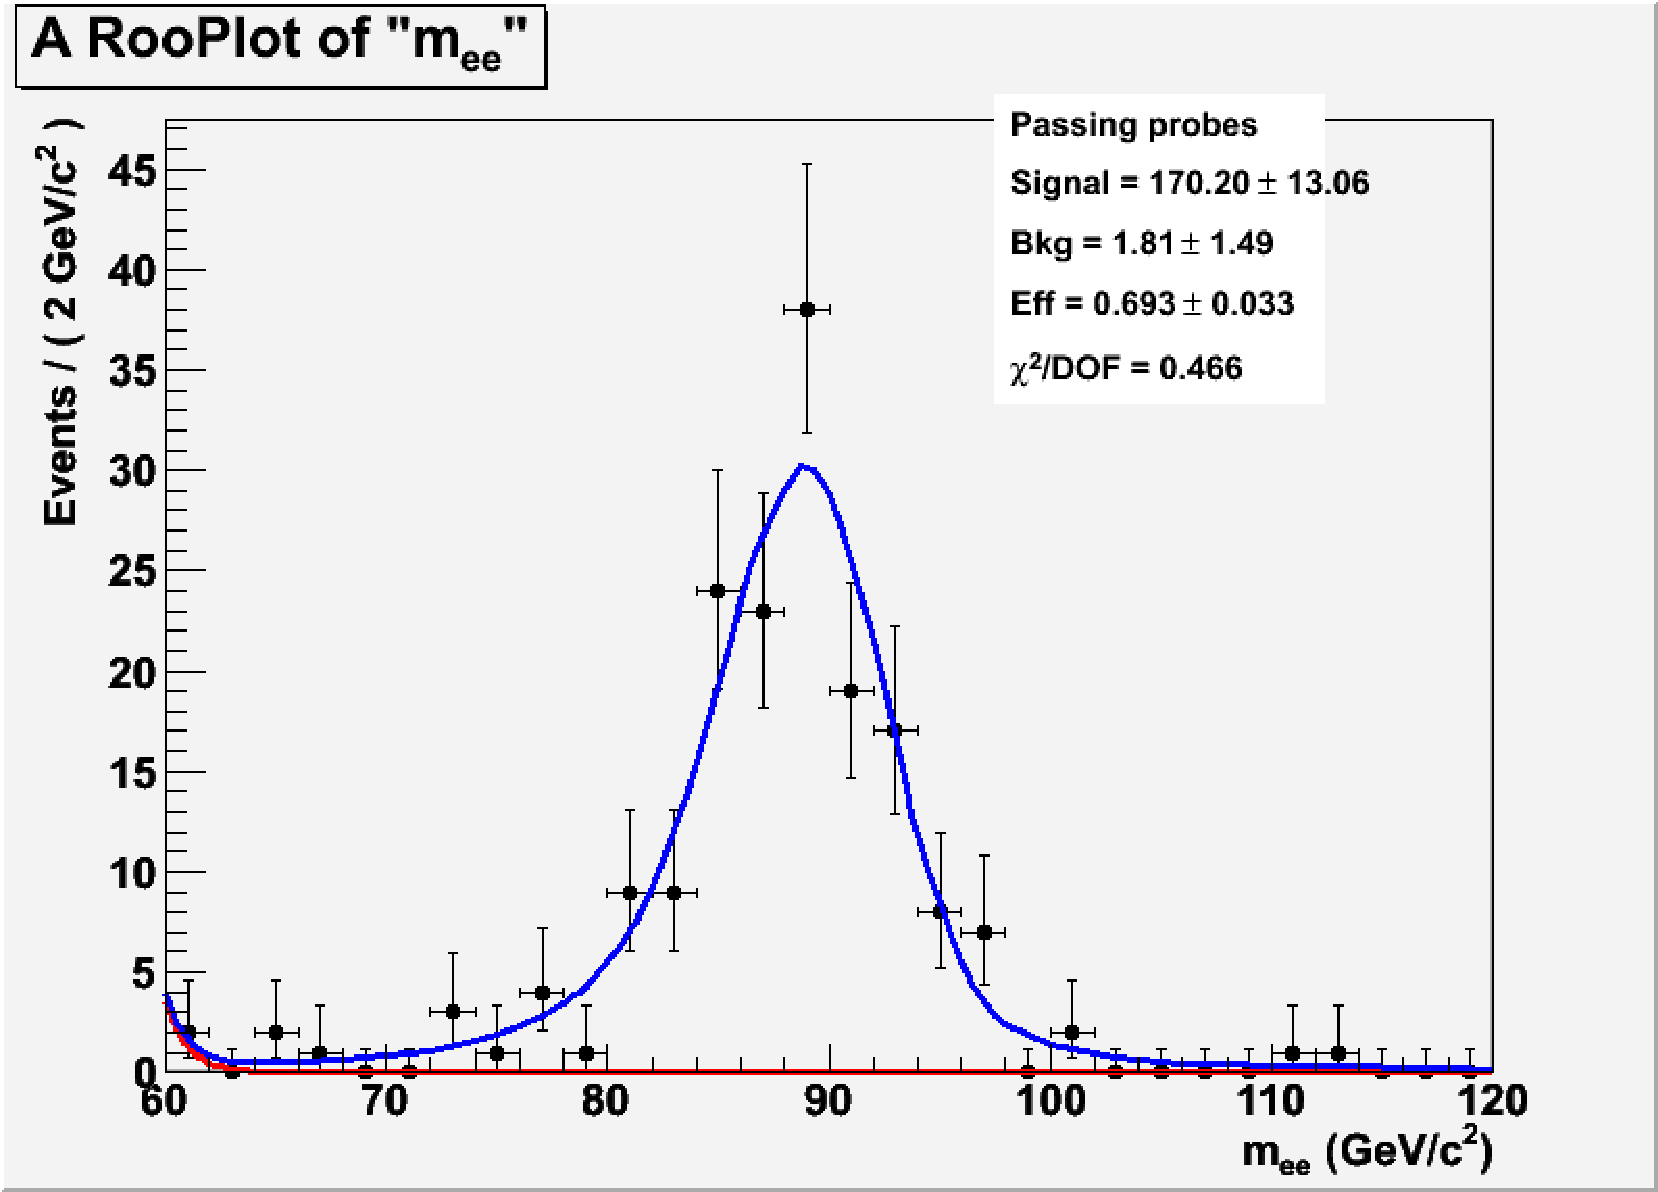
\includegraphics[width=0.49\textwidth]{Efficiency_RecoToVBTF80_MCSignalShape_EE_Minus_Pass.pdf}}
    \subfigure[]{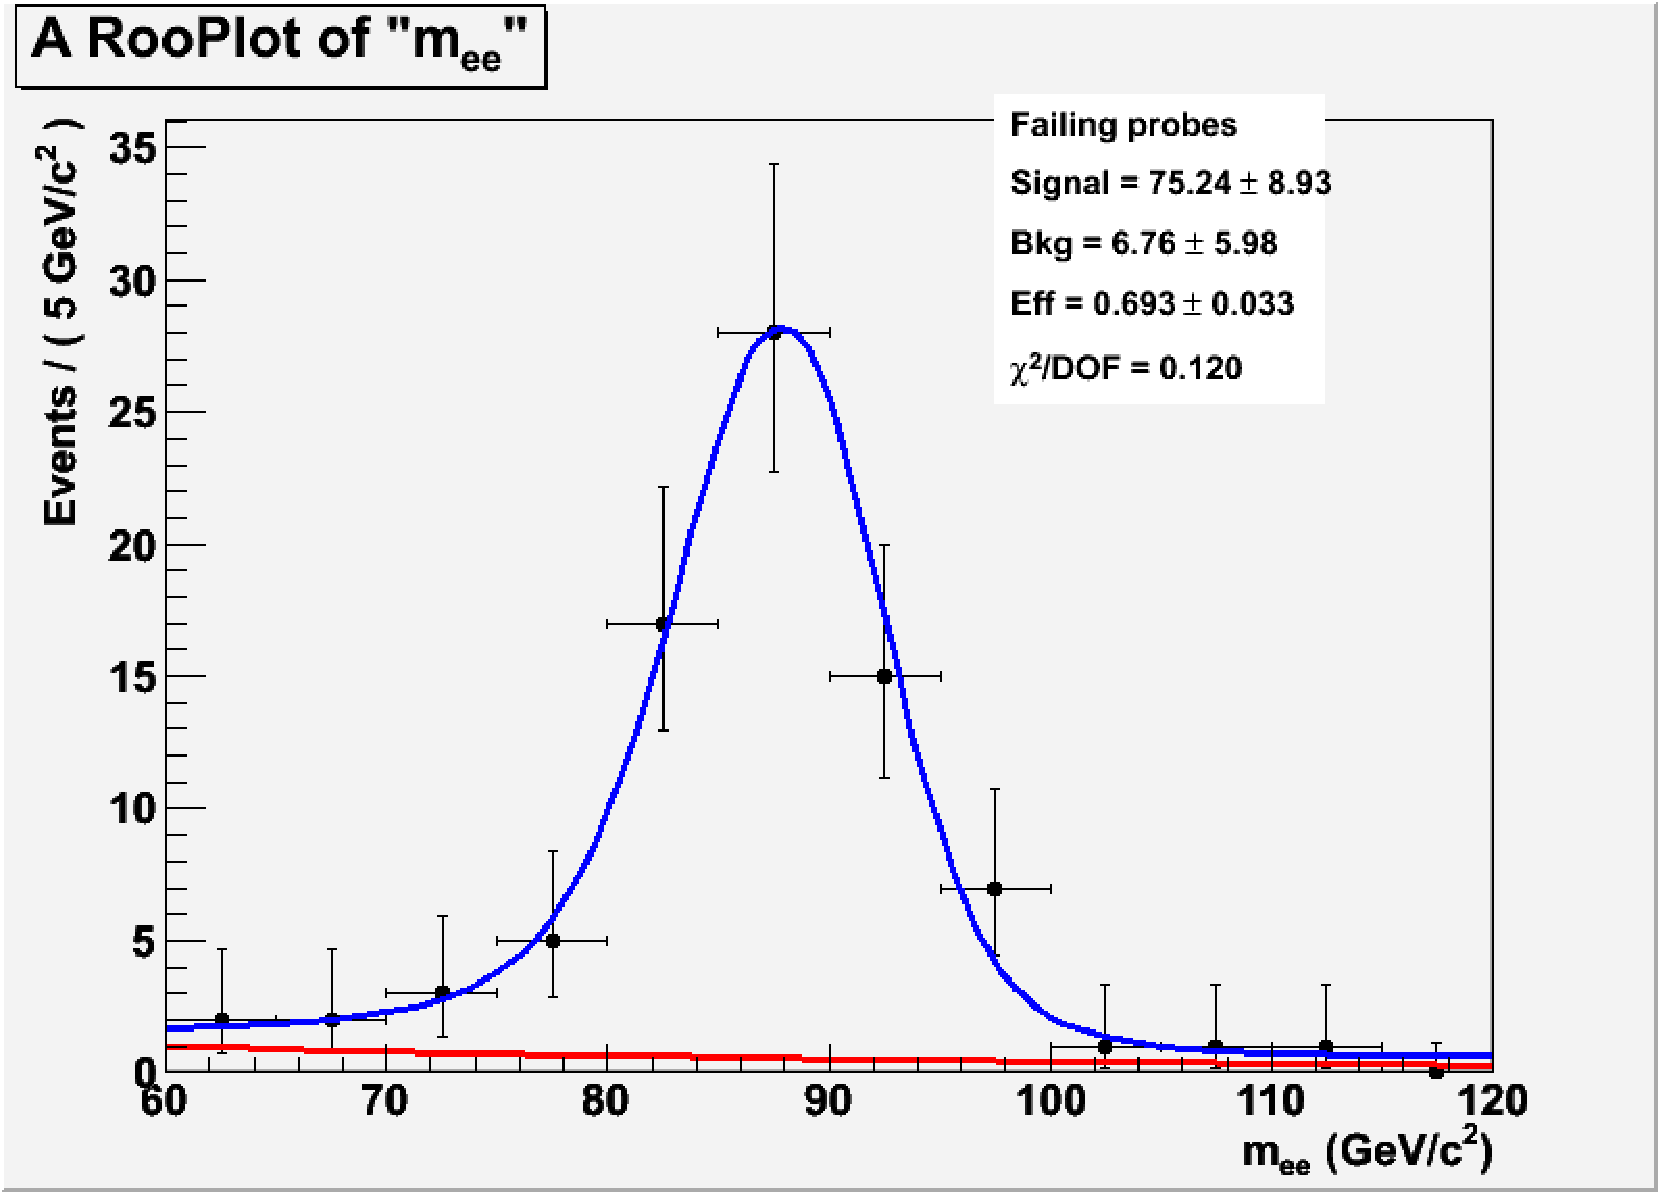
\includegraphics[width=0.49\textwidth]{Efficiency_RecoToVBTF80_MCSignalShape_EE_Minus_Fail.pdf}}
    \caption{The passing (a) and failing (b) fits for the Reco$\to$WP80 step in the Ecal Barrel for electrons.
             The data is in black, background fit in red, and signal+background fit in blue.}
  \end{center}
\end{figure}

\begin{figure}[htb]
  \begin{center}
    \subfigure[]{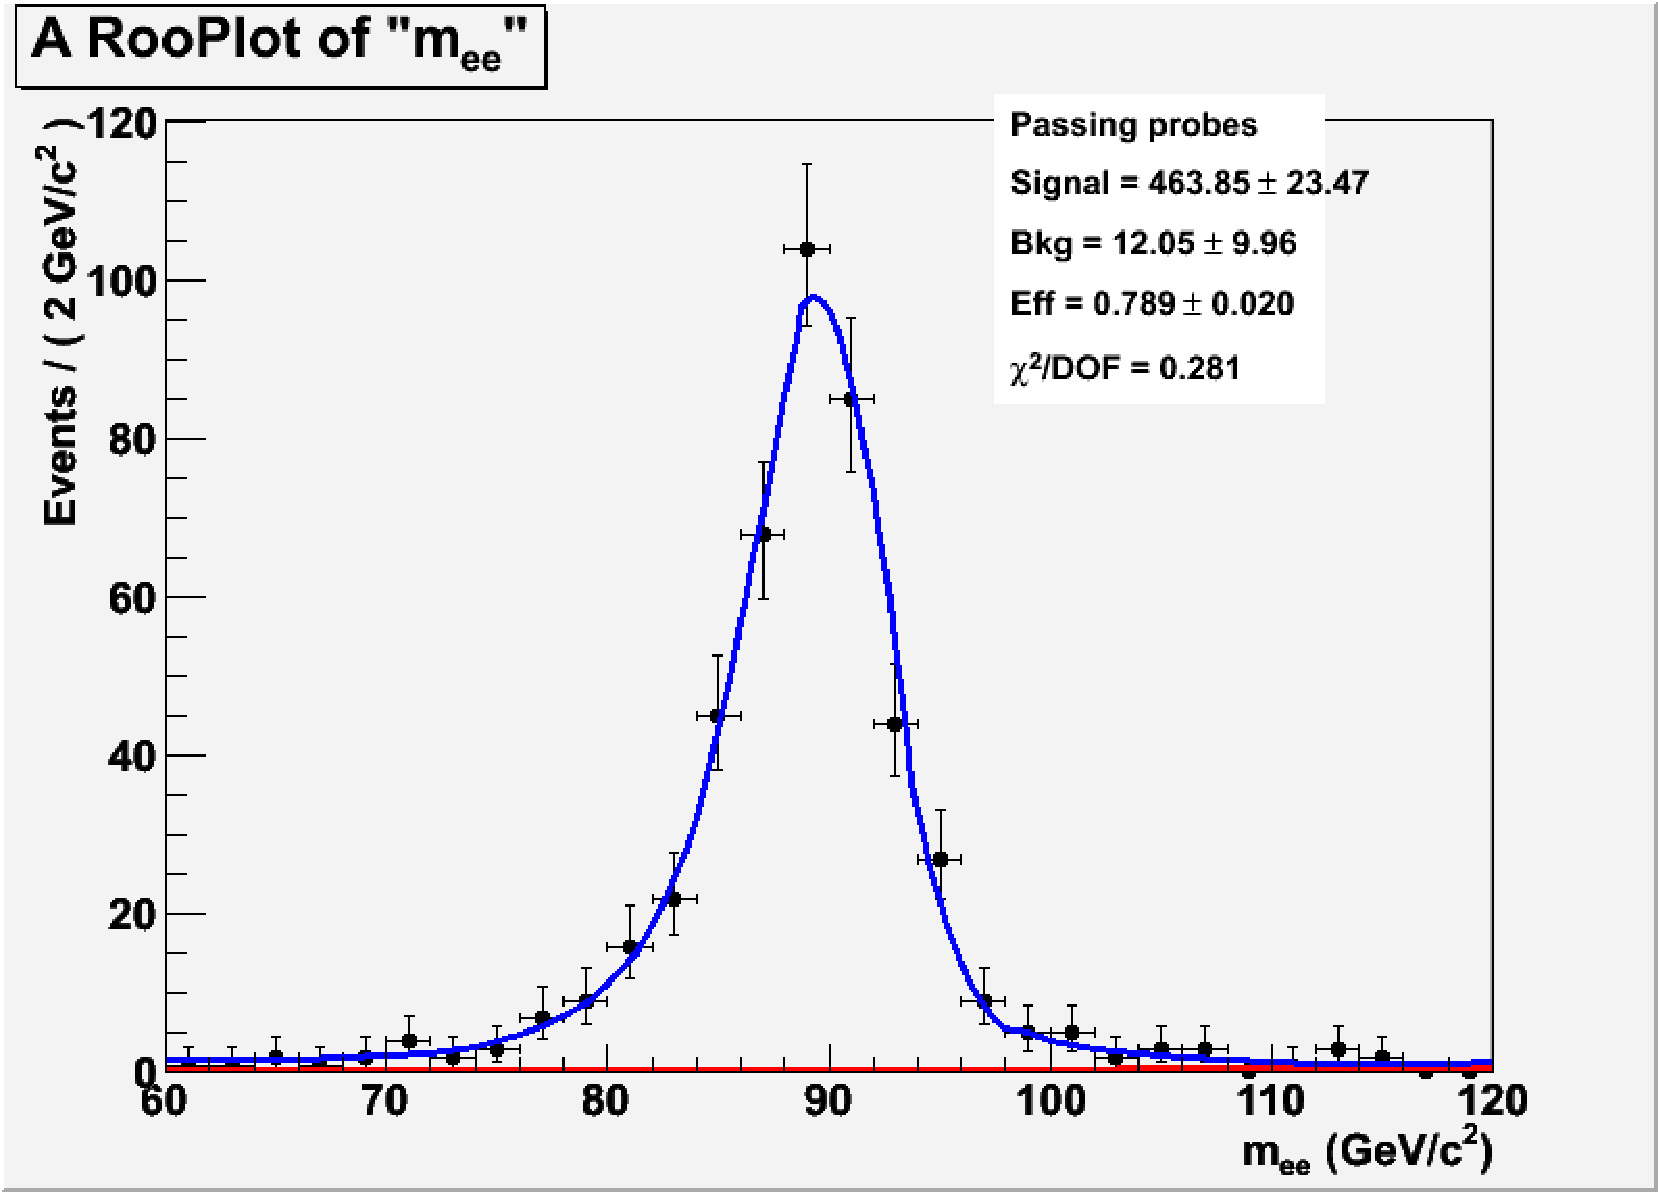
\includegraphics[width=0.49\textwidth]{Efficiency_RecoToVBTF80_MCSignalShape_EB_Plus_Pass.pdf}}
    \subfigure[]{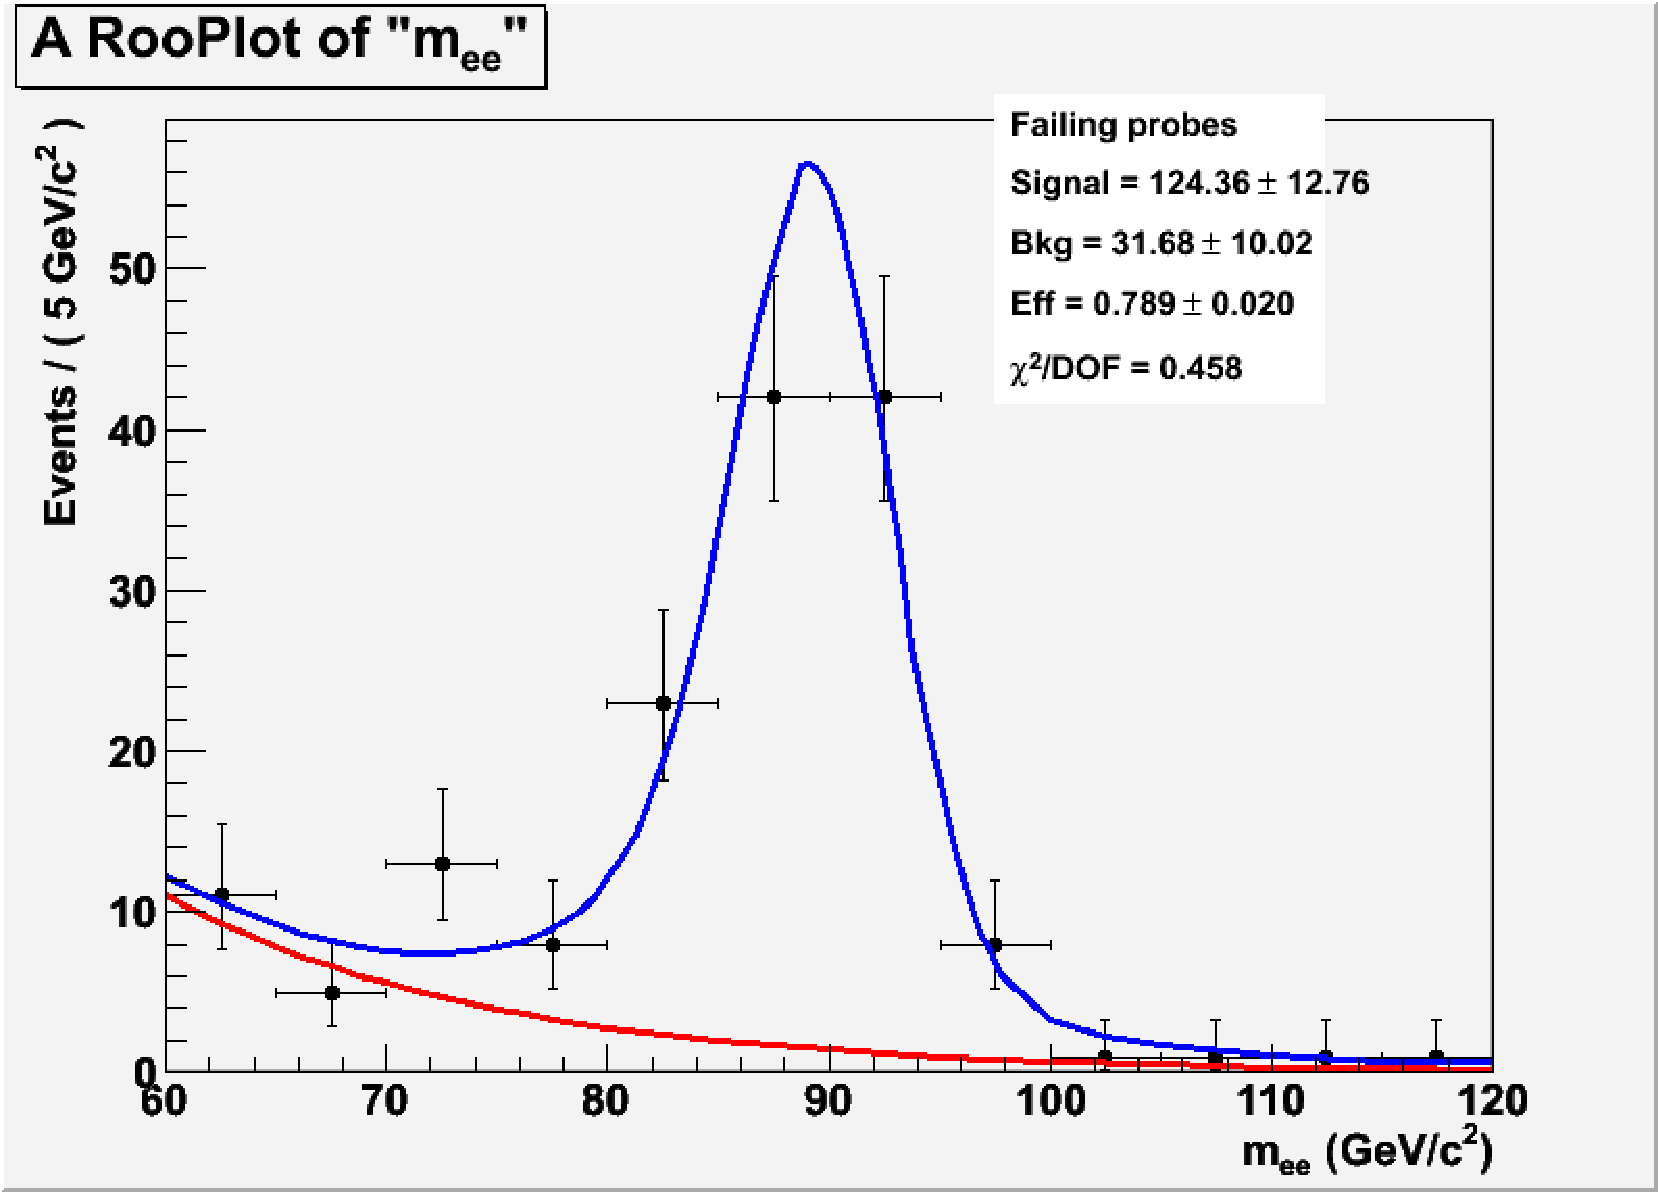
\includegraphics[width=0.49\textwidth]{Efficiency_RecoToVBTF80_MCSignalShape_EB_Plus_Fail.pdf}}
    \caption{The passing (a) and failing (b) fits for the Reco$\to$WP80 step in the Ecal Barrel for positrons.
             The data is in black, background fit in red, and signal+background fit in blue.}
  \end{center}
\end{figure}

\begin{figure}[htb]
  \begin{center}
    \subfigure[]{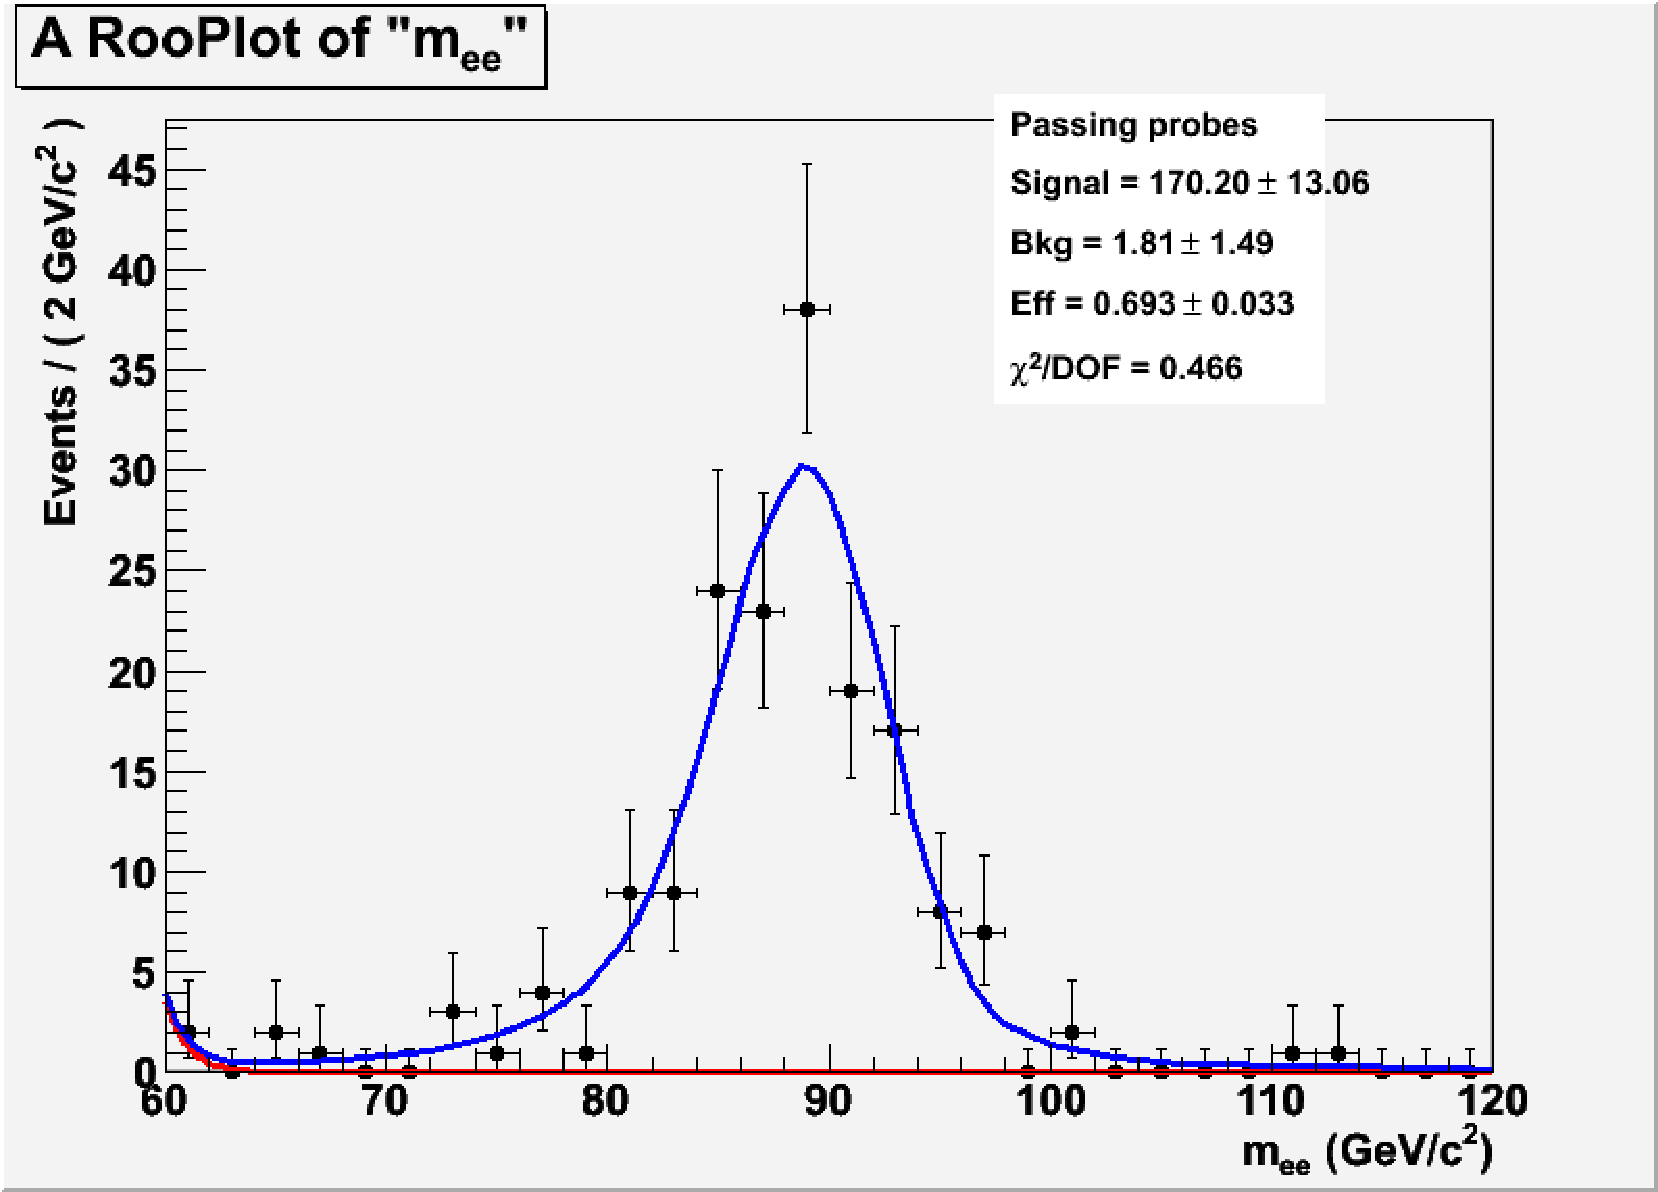
\includegraphics[width=0.49\textwidth]{Efficiency_RecoToVBTF80_MCSignalShape_EE_Minus_Pass.pdf}}
    \subfigure[]{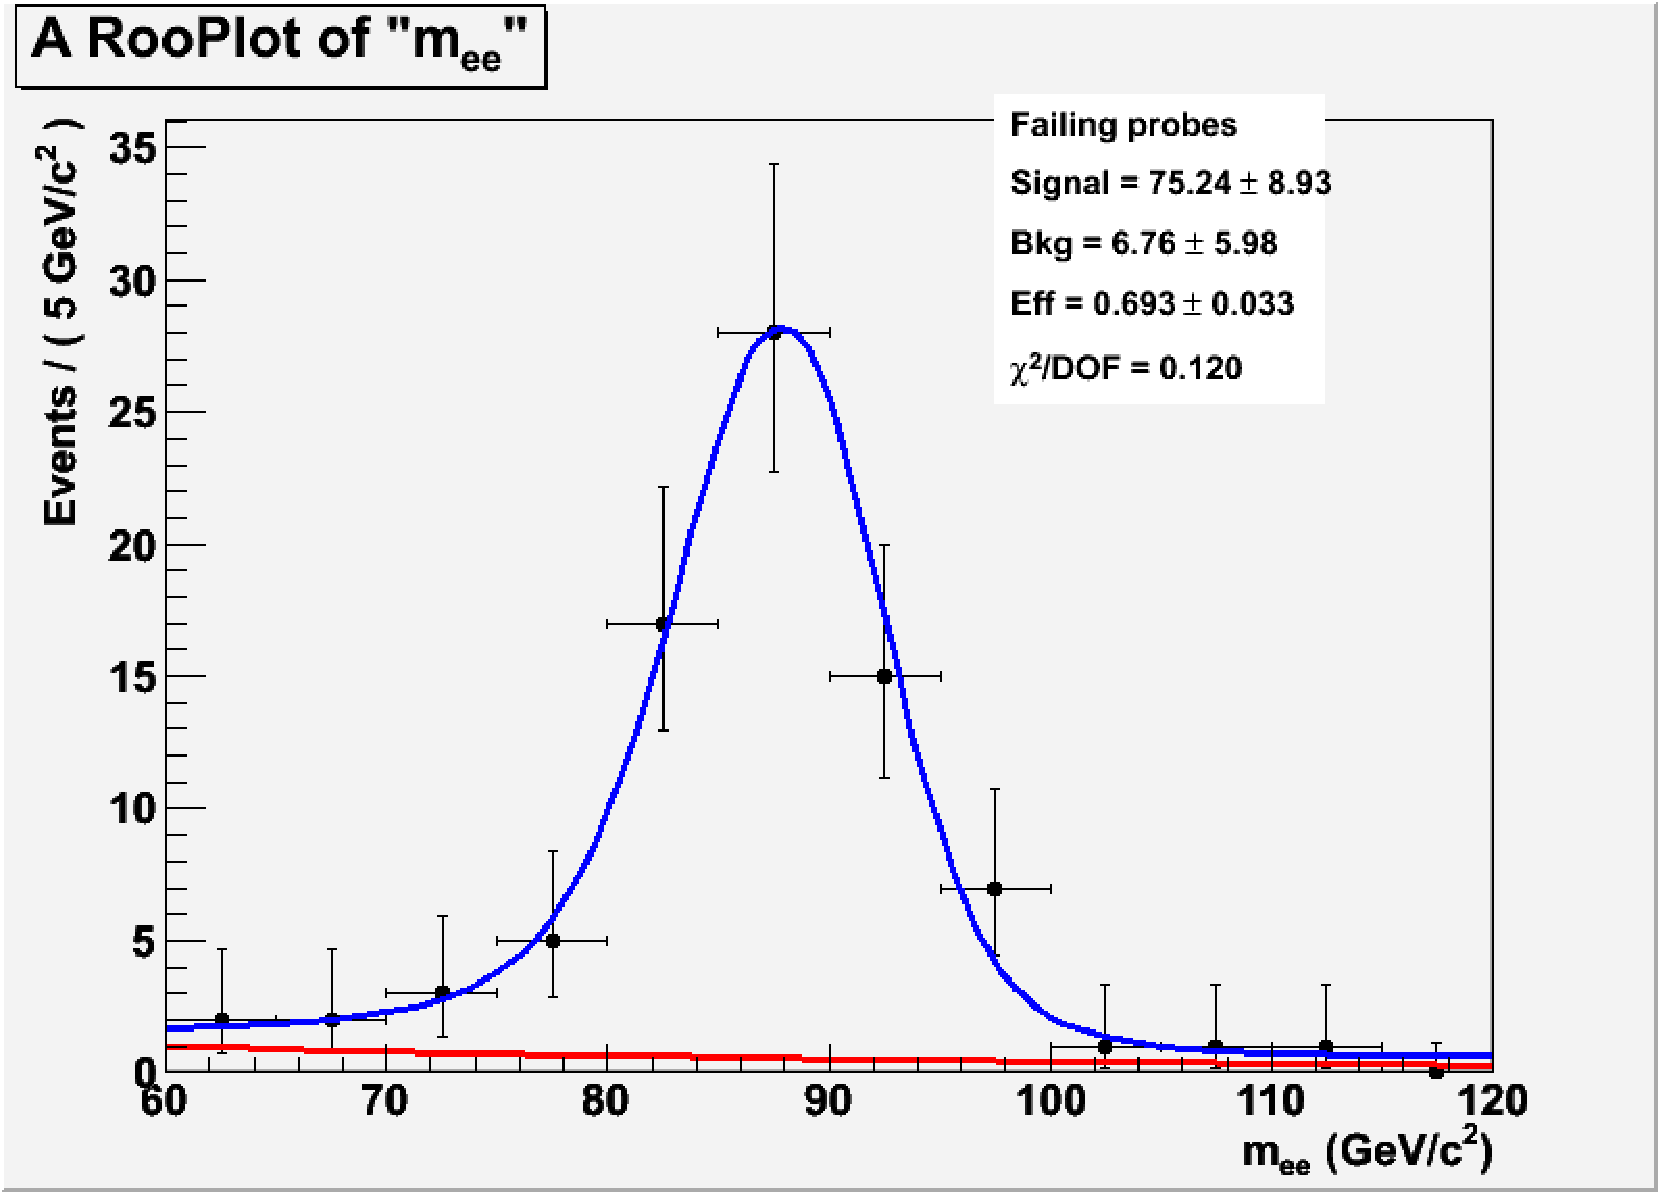
\includegraphics[width=0.49\textwidth]{Efficiency_RecoToVBTF80_MCSignalShape_EE_Minus_Fail.pdf}}
    \caption{The passing (a) and failing (b) fits for the Reco$\to$WP80 step in the Ecal Endcap for electrons.
             The data is in black, background fit in red, and signal+background fit in blue.}
  \end{center}
\end{figure}

\begin{figure}[htb]
  \begin{center}
    \subfigure[]{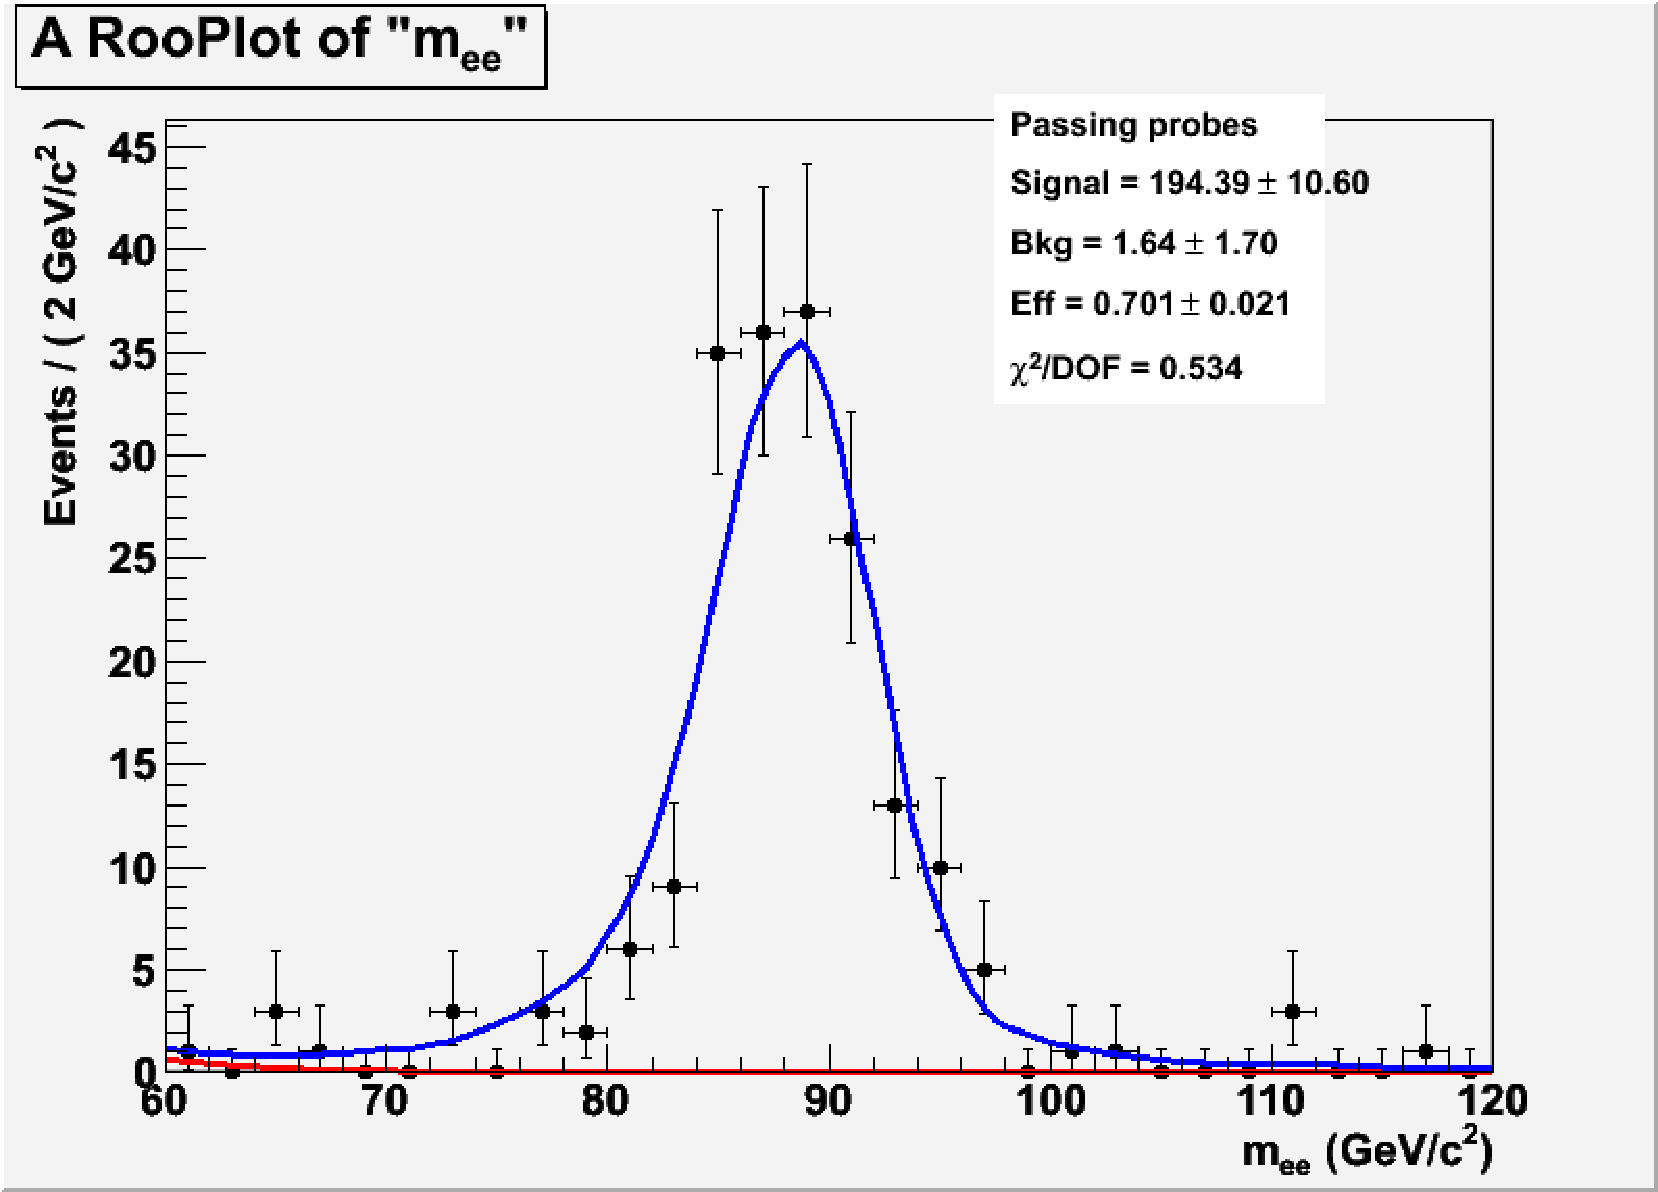
\includegraphics[width=0.49\textwidth]{Efficiency_RecoToVBTF80_MCSignalShape_EE_Plus_Pass.pdf}}
    \subfigure[]{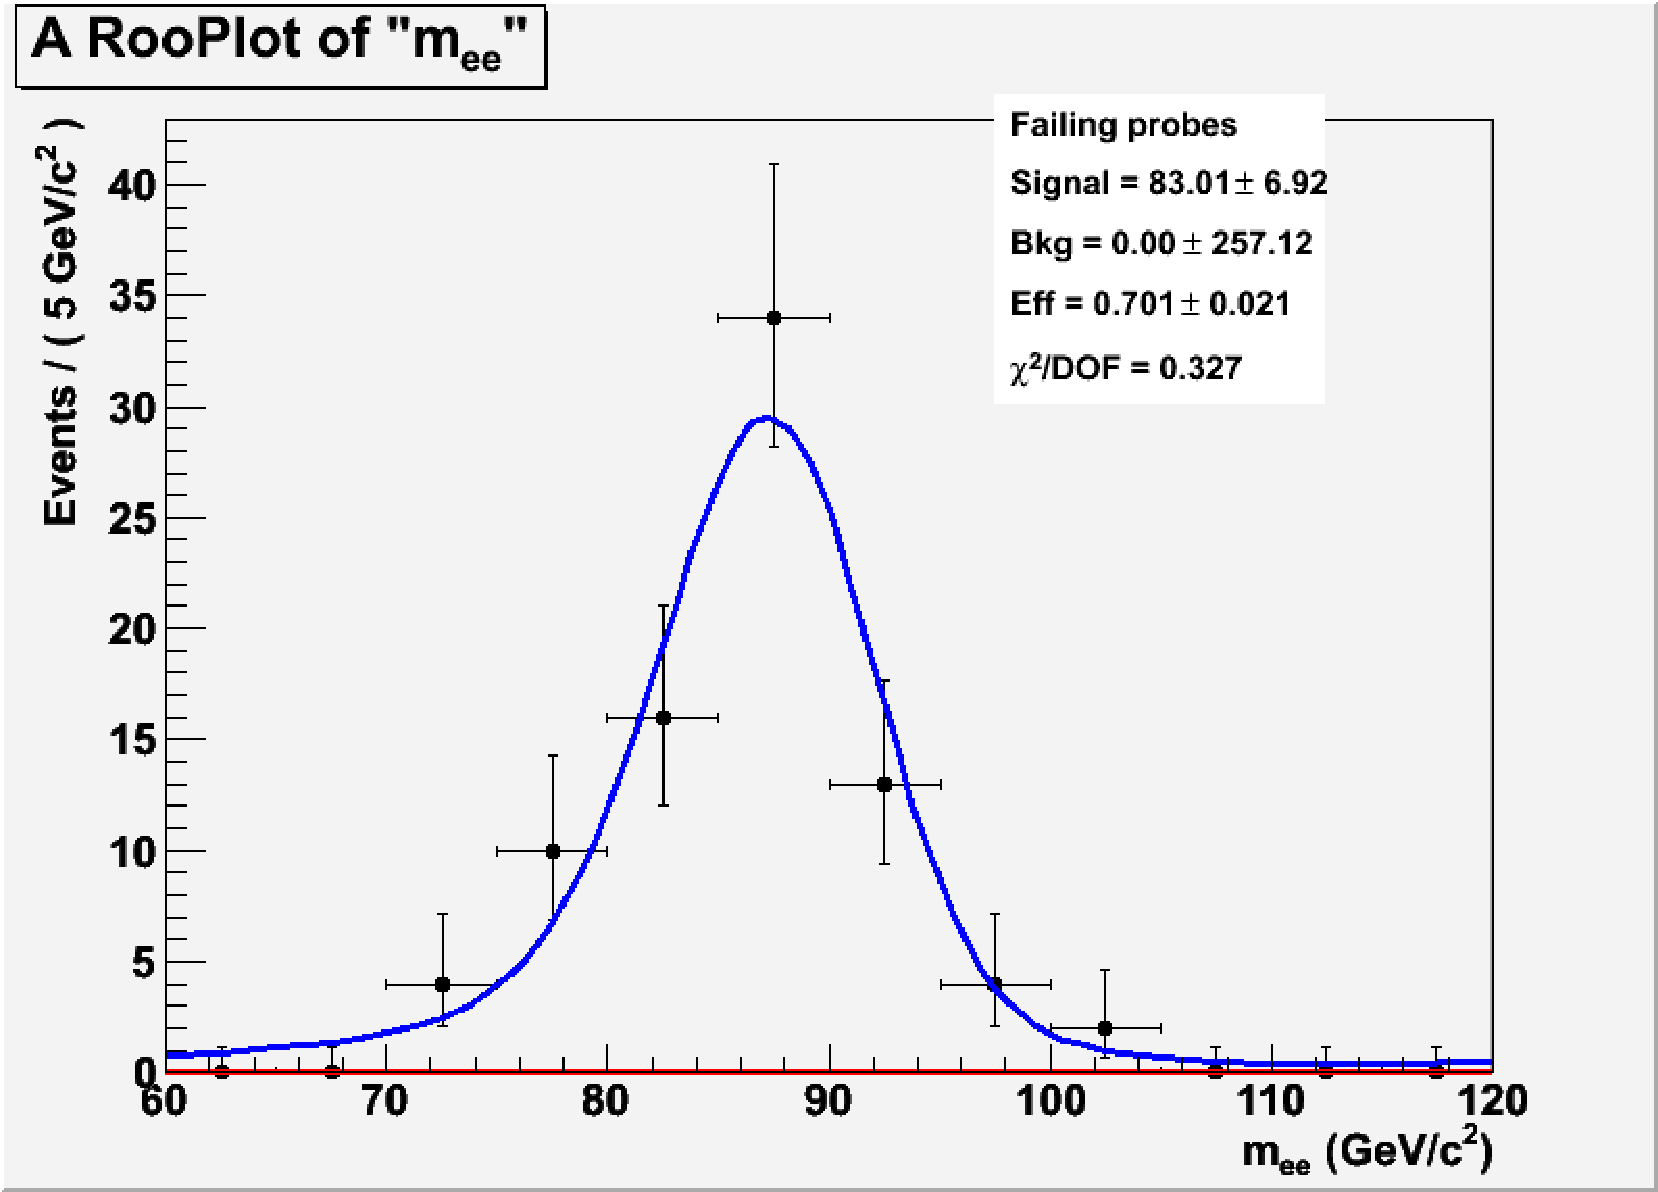
\includegraphics[width=0.49\textwidth]{Efficiency_RecoToVBTF80_MCSignalShape_EE_Plus_Fail.pdf}}
    \caption{The passing (a) and failing (b) fits for the Reco$\to$WP80 step in the Ecal Endcap for positrons.
             The data is in black, background fit in red, and signal+background fit in blue.}
  \end{center}
\end{figure}

\clearpage
\newpage

\section{Generator-Level Signal Shape Fit Plots }
\label{genShapePlots}

%sc->reco
\begin{figure}[htb]
  \begin{center}
    \subfigure[]{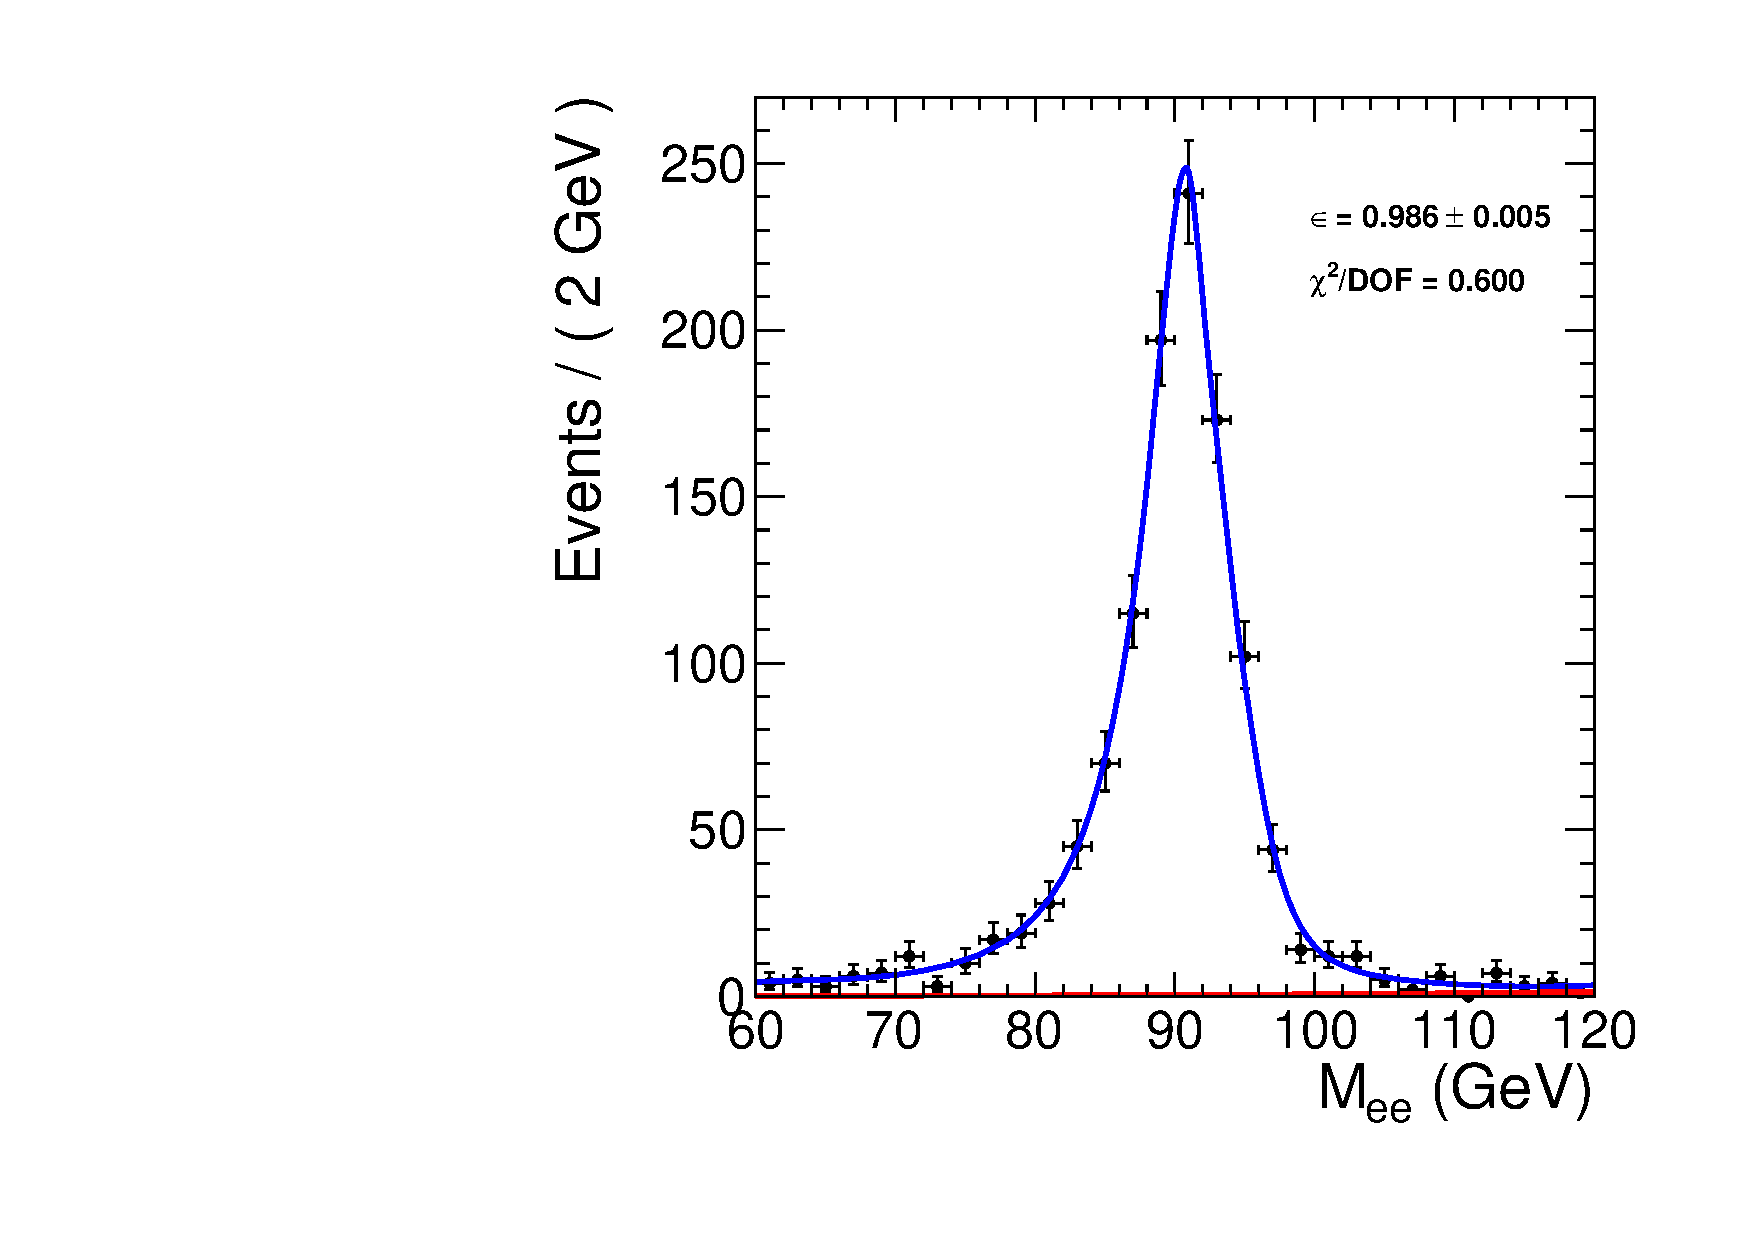
\includegraphics[width=0.49\textwidth]{tpHistos_GSF_eb_pass.pdf}}
    \subfigure[]{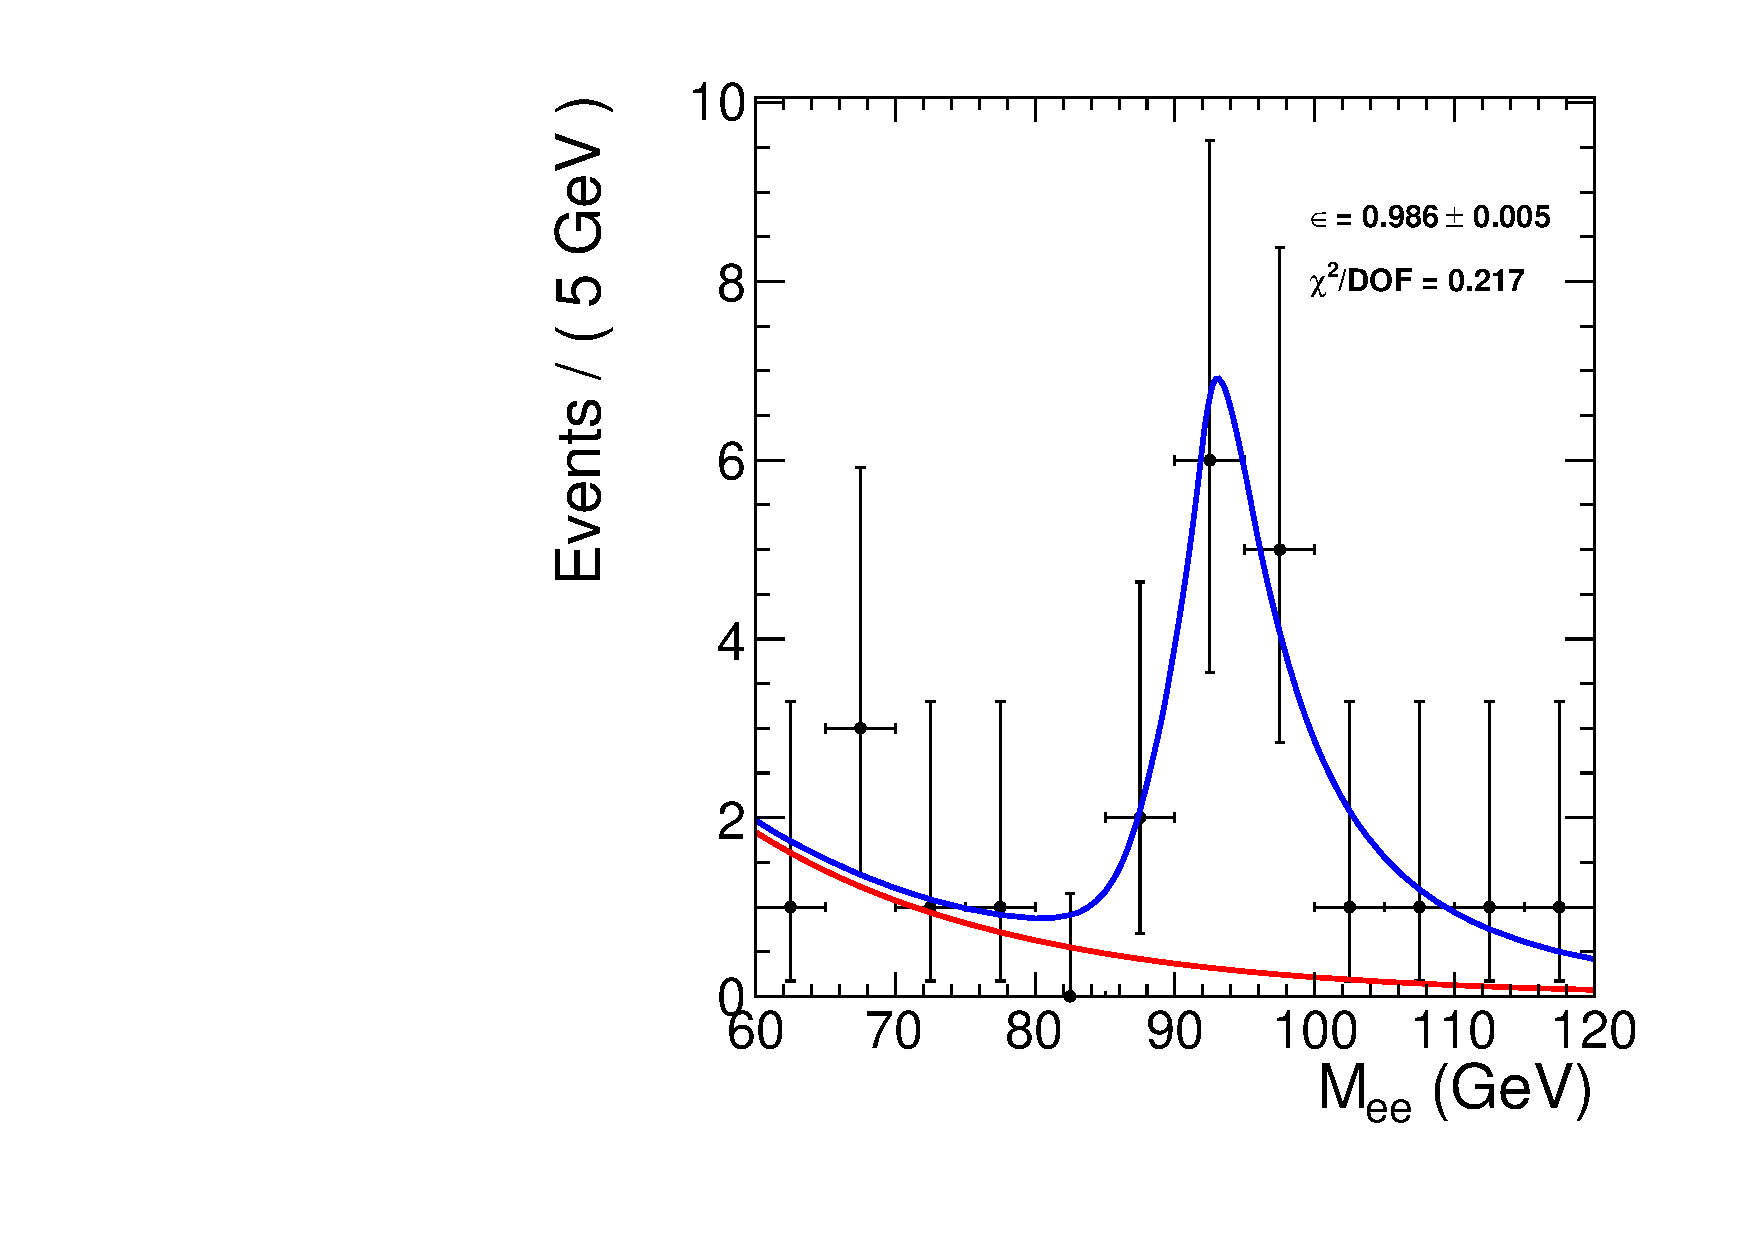
\includegraphics[width=0.49\textwidth]{tpHistos_GSF_eb_fail.pdf}}
    \caption{The passing (a) and failing (b) fits for the SC$\to$Reco step in the Ecal Barrel.
             The data is in black, background fit in red, and signal+background fit in blue.}
  \end{center}
\end{figure}

\begin{figure}[htb]
  \begin{center}
    \subfigure[]{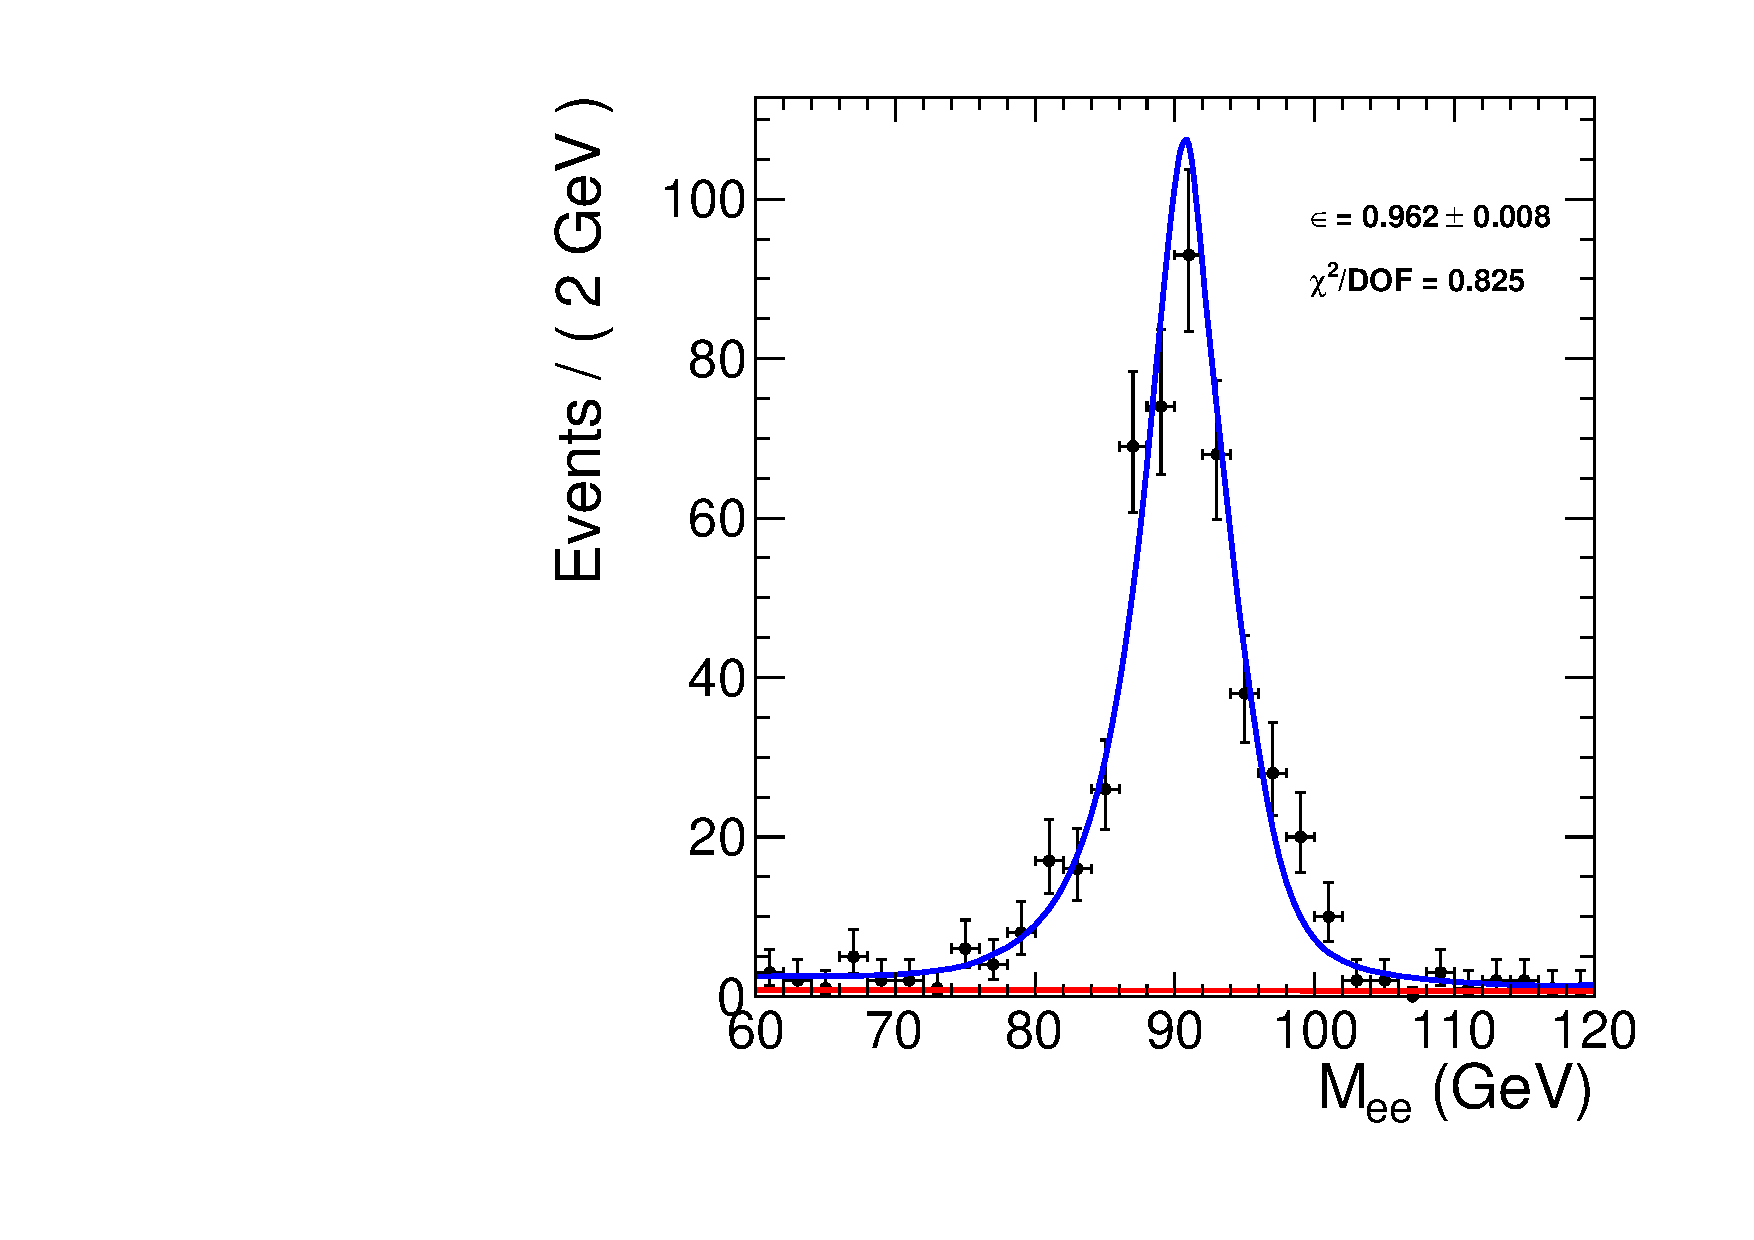
\includegraphics[width=0.49\textwidth]{tpHistos_GSF_ee_pass.pdf}}
    \subfigure[]{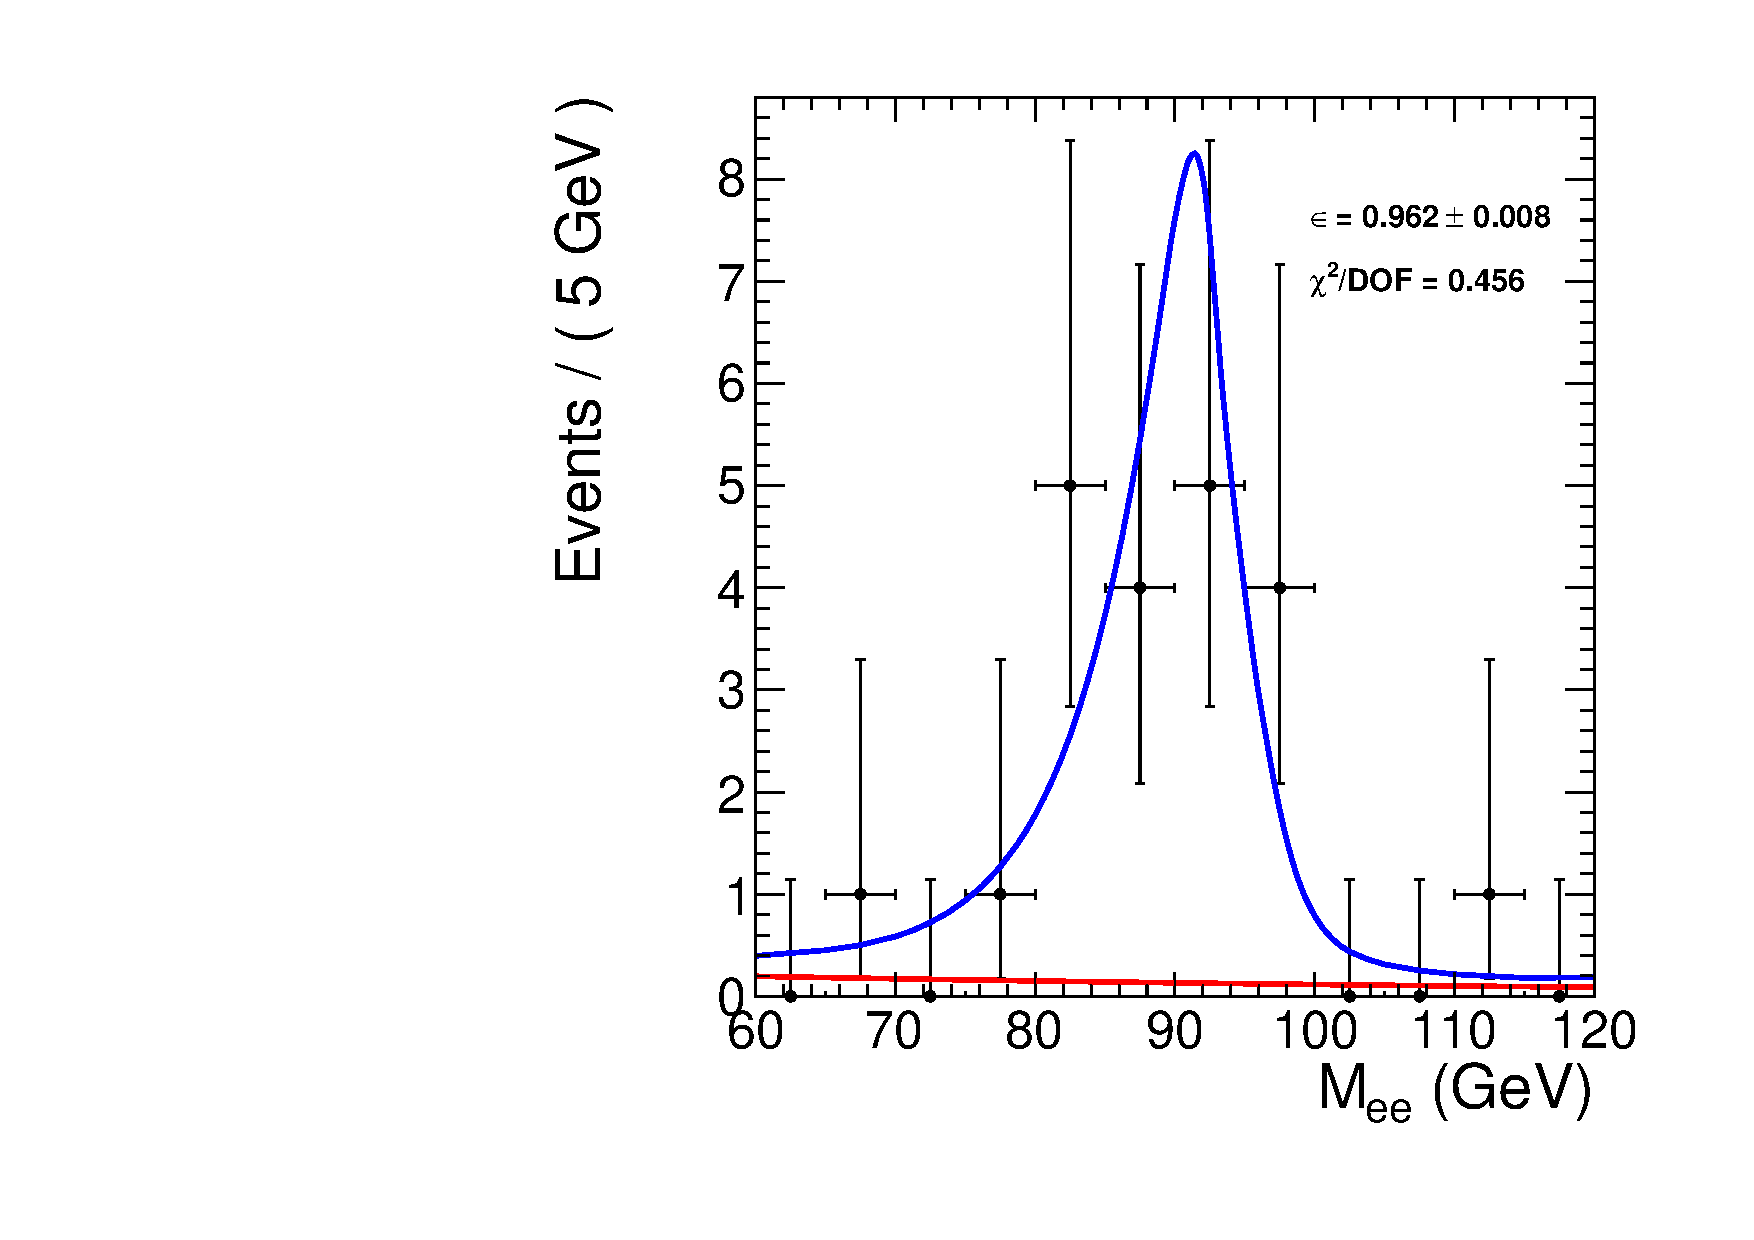
\includegraphics[width=0.49\textwidth]{tpHistos_GSF_ee_fail.pdf}}
    \caption{The passing (a) and failing (b) fits for the SC$\to$Reco step in the Ecal Endcap.  
             The data is in black, background fit in red, and signal+background fit in blu\
e.}
  \end{center}
\end{figure}

\begin{figure}[htb]
  \begin{center}
    \subfigure[]{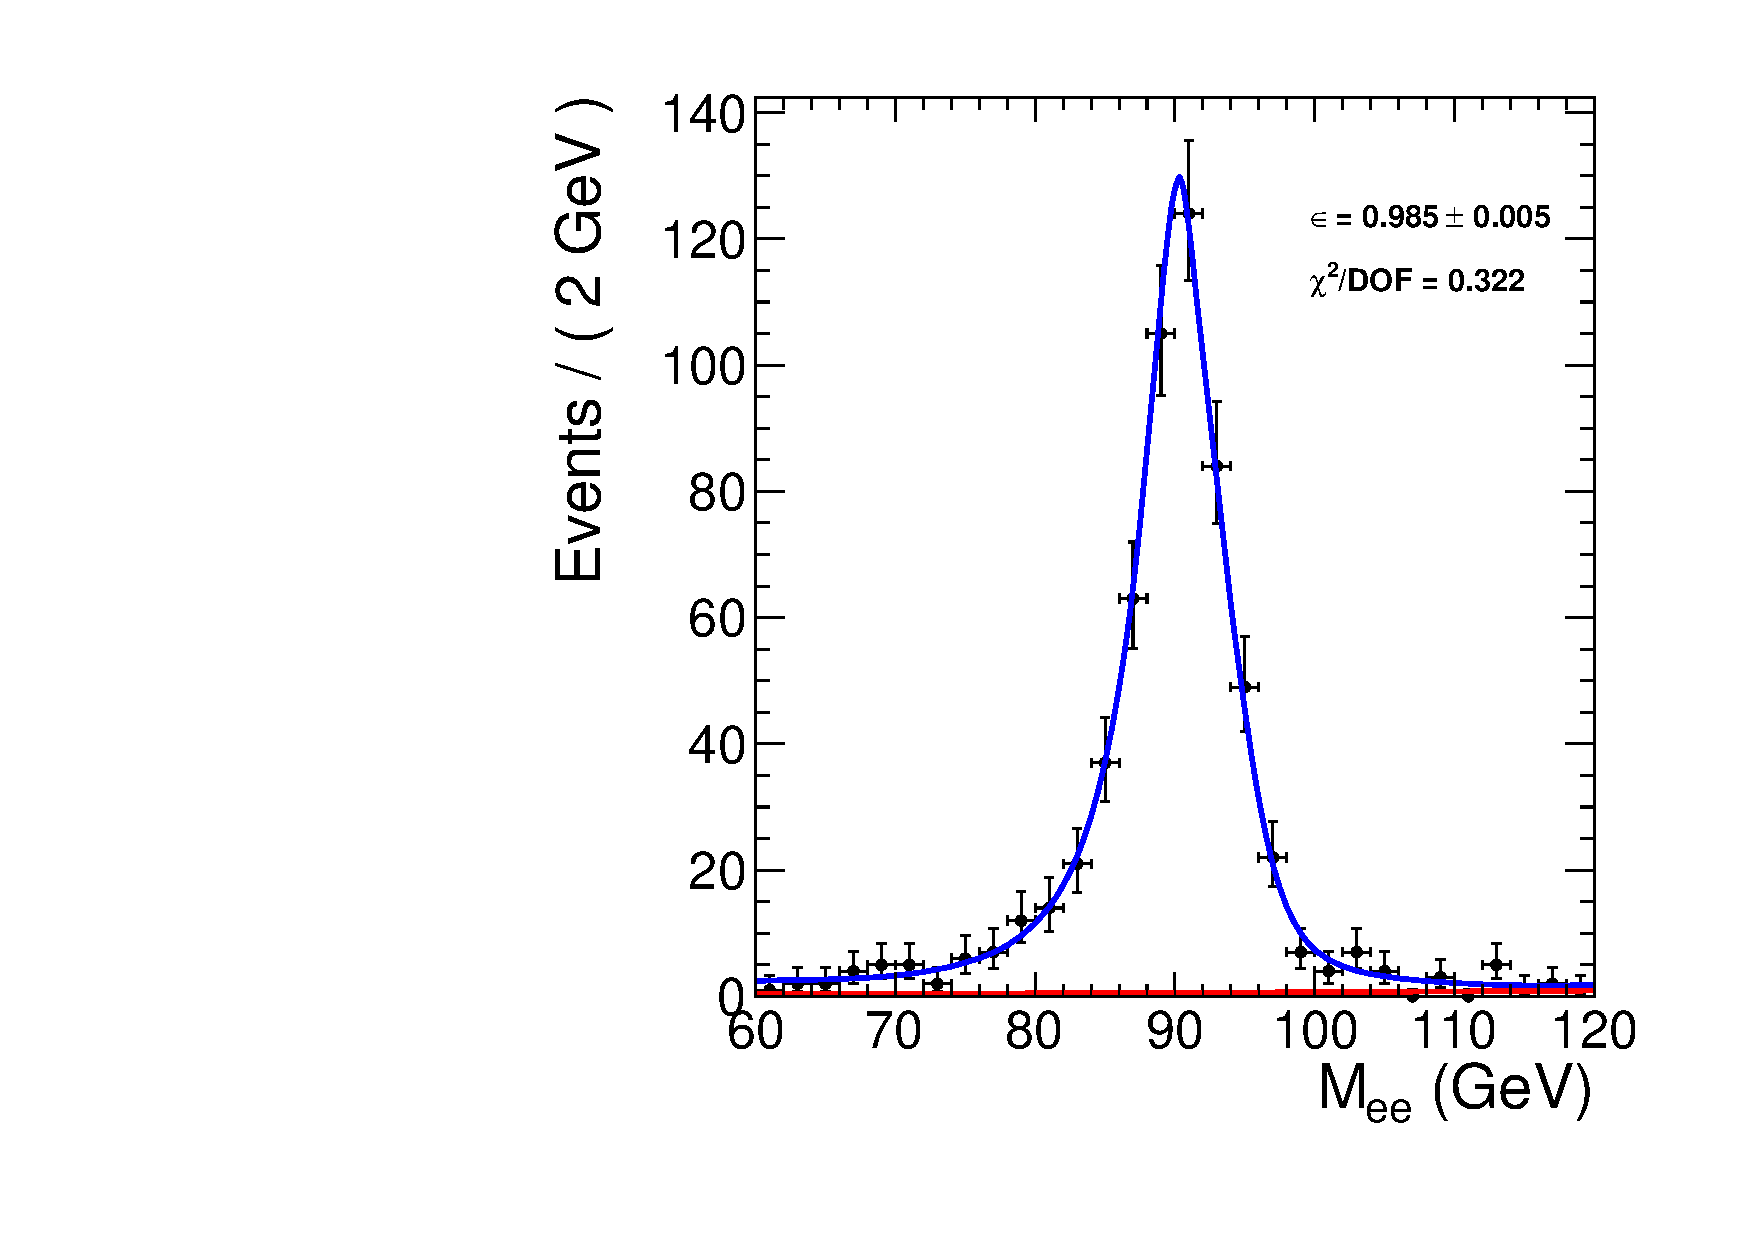
\includegraphics[width=0.49\textwidth]{tpHistos_GSF_eb_minus_pass.pdf}}
    \subfigure[]{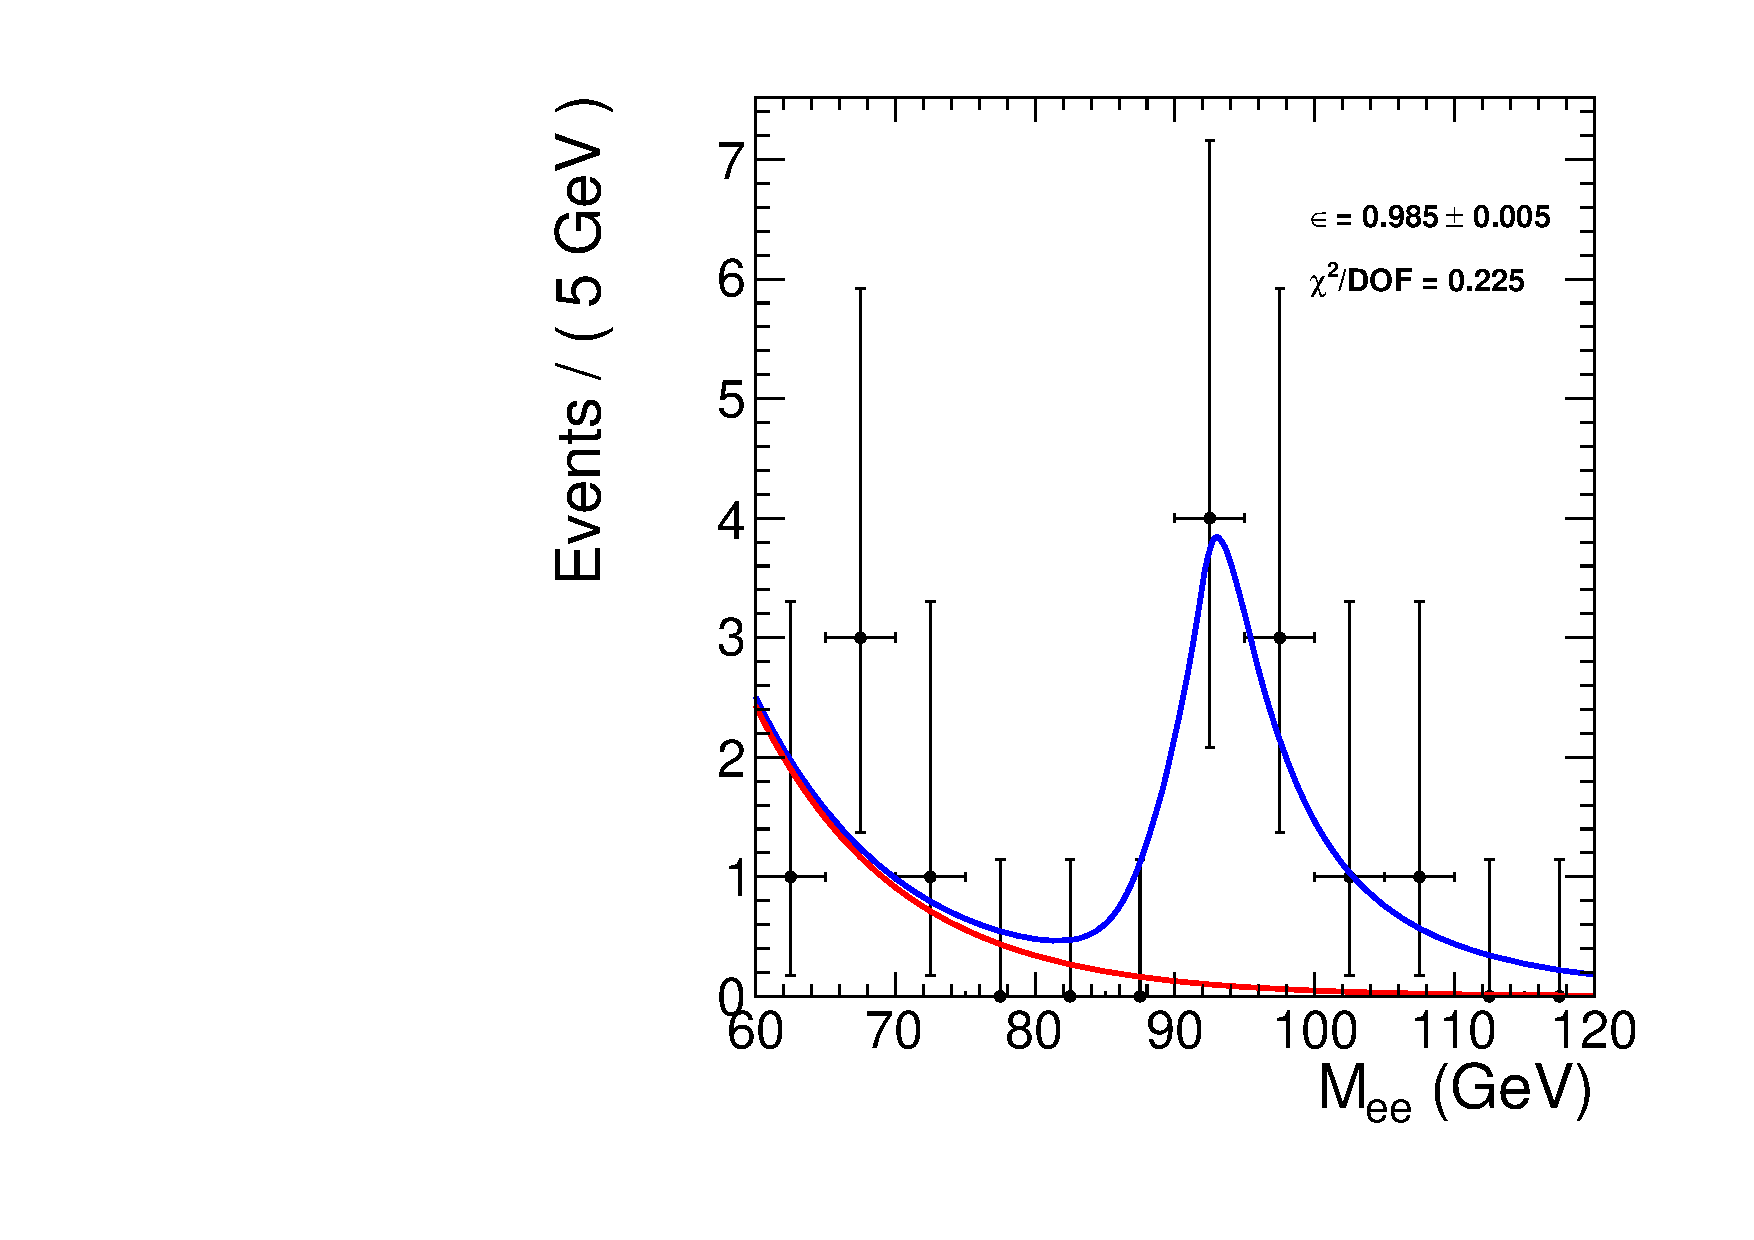
\includegraphics[width=0.49\textwidth]{tpHistos_GSF_eb_minus_fail.pdf}}
    \caption{The passing (a) and failing (b) fits for the SC$\to$Reco step in the Ecal Barrel for electrons.
             The data is in black, background fit in red, and signal+background fit in blue.}
  \end{center}
\end{figure}

\begin{figure}[htb]
  \begin{center}
    \subfigure[]{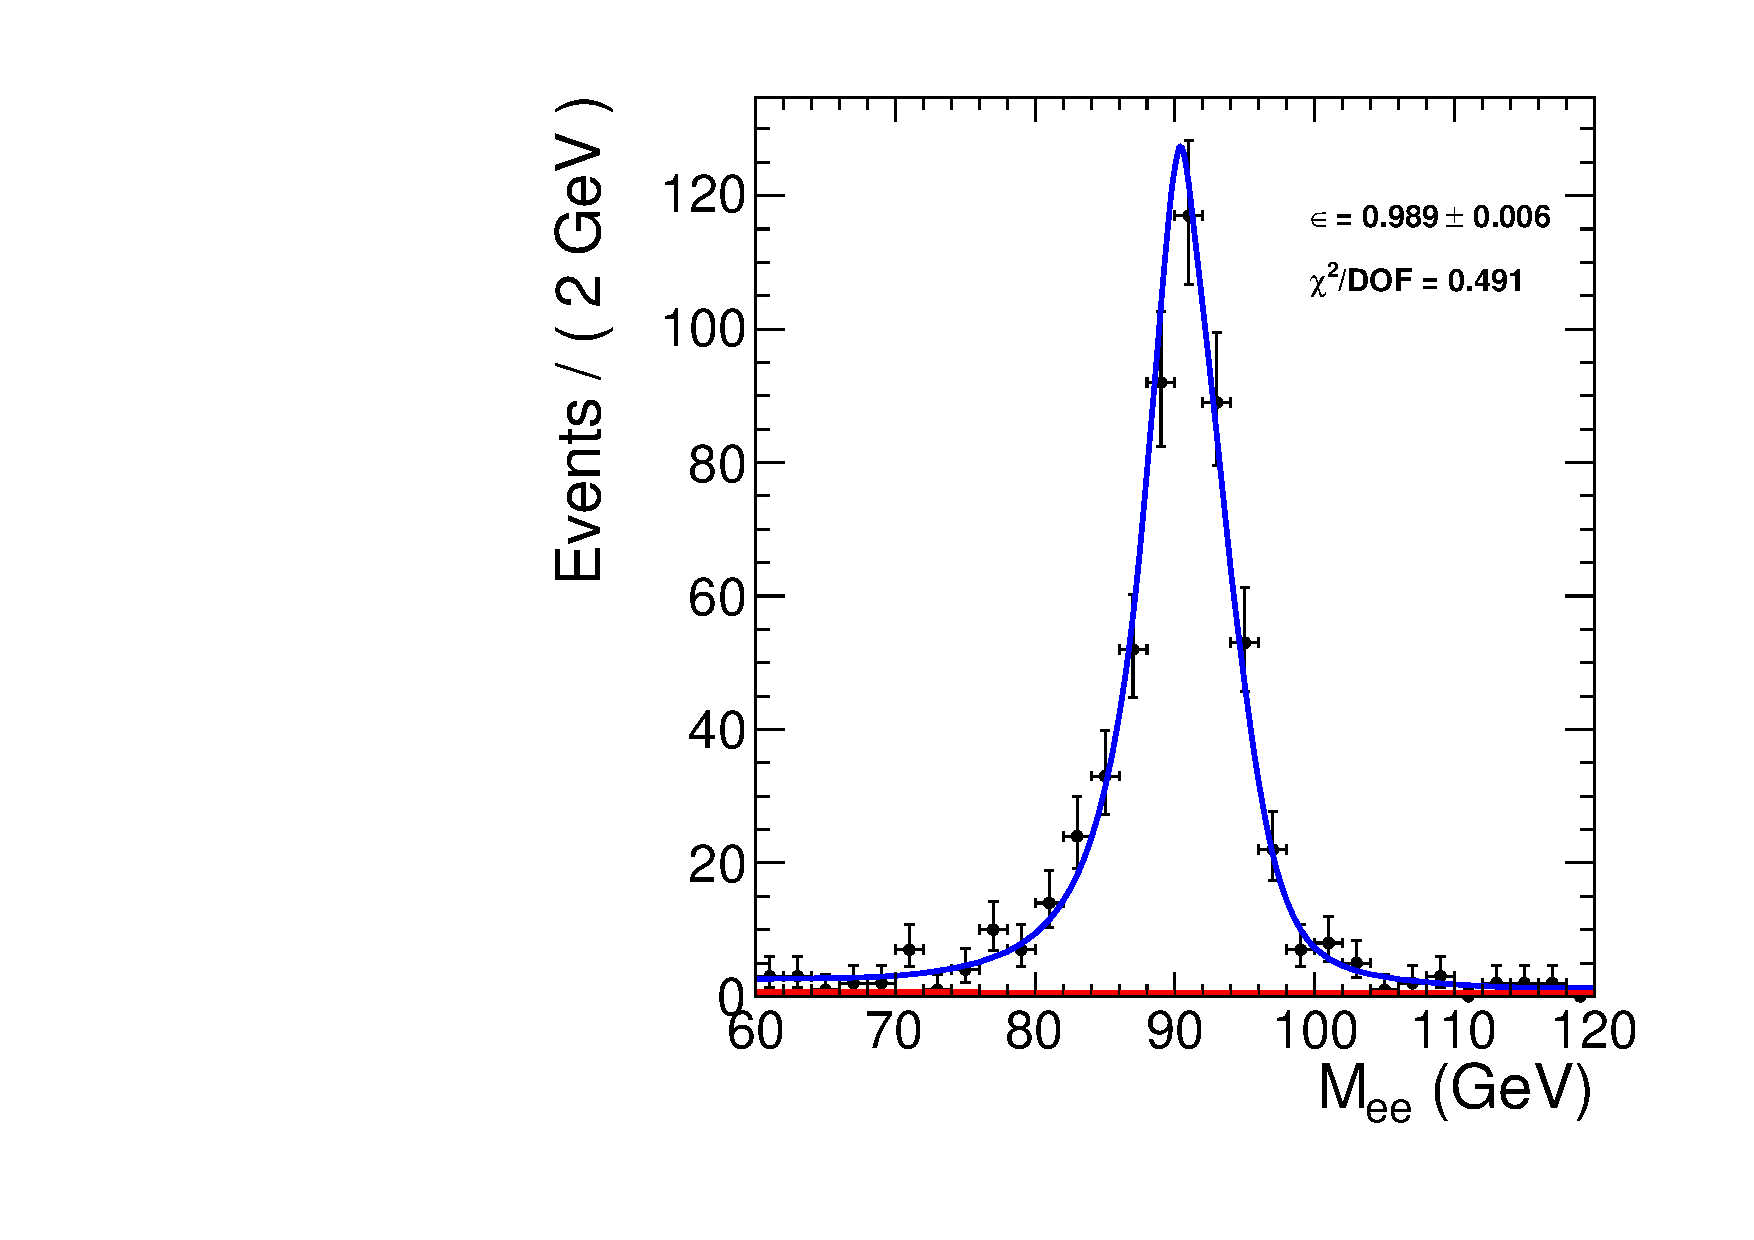
\includegraphics[width=0.49\textwidth]{tpHistos_GSF_eb_plus_pass.pdf}}
    \subfigure[]{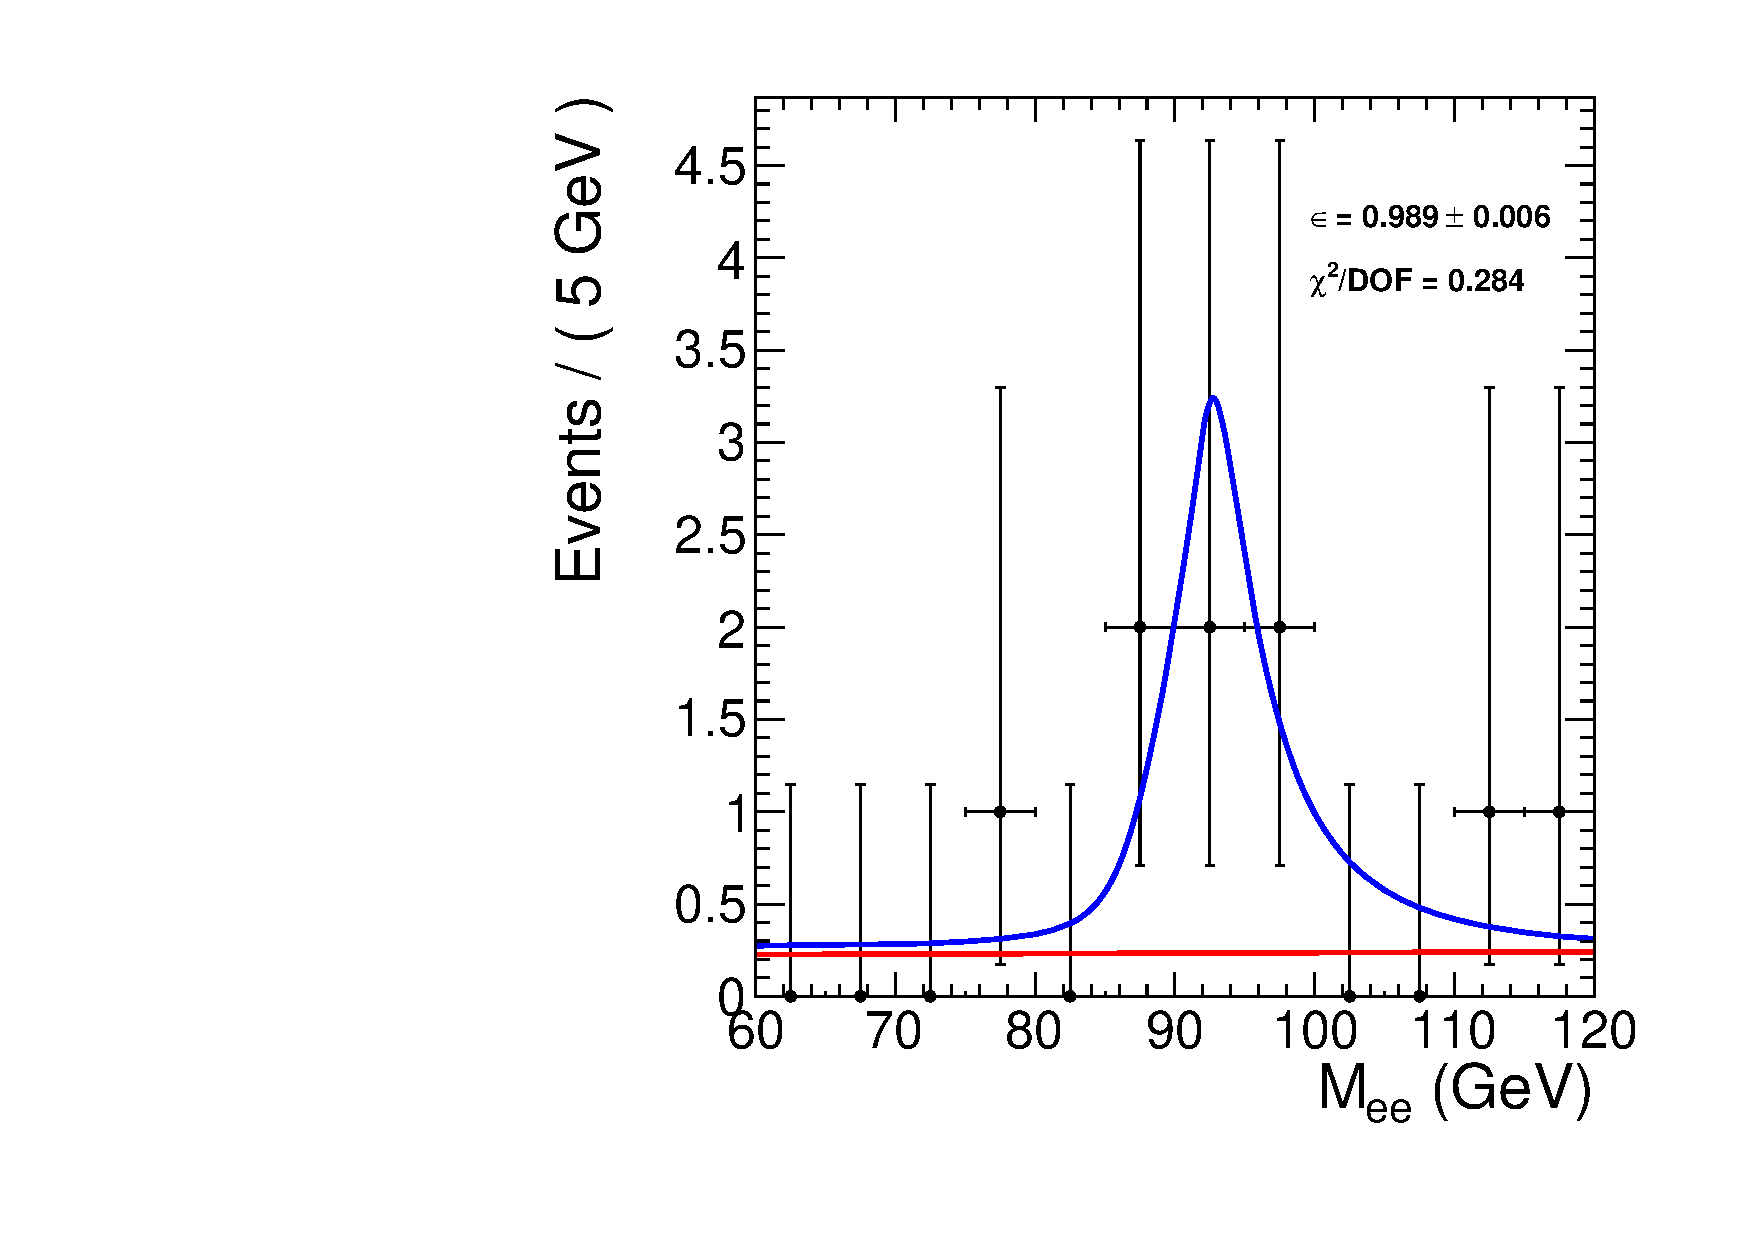
\includegraphics[width=0.49\textwidth]{tpHistos_GSF_eb_plus_fail.pdf}}
    \caption{The passing (a) and failing (b) fits for the SC$\to$Reco step in the Ecal Barrel for positrons.
             The data is in black, background fit in red, and signal+background fit in blue.}
  \label{fig:scRecoEbPlus}  
  \end{center}
\end{figure}

\begin{figure}[htb]
  \begin{center}
    \subfigure[]{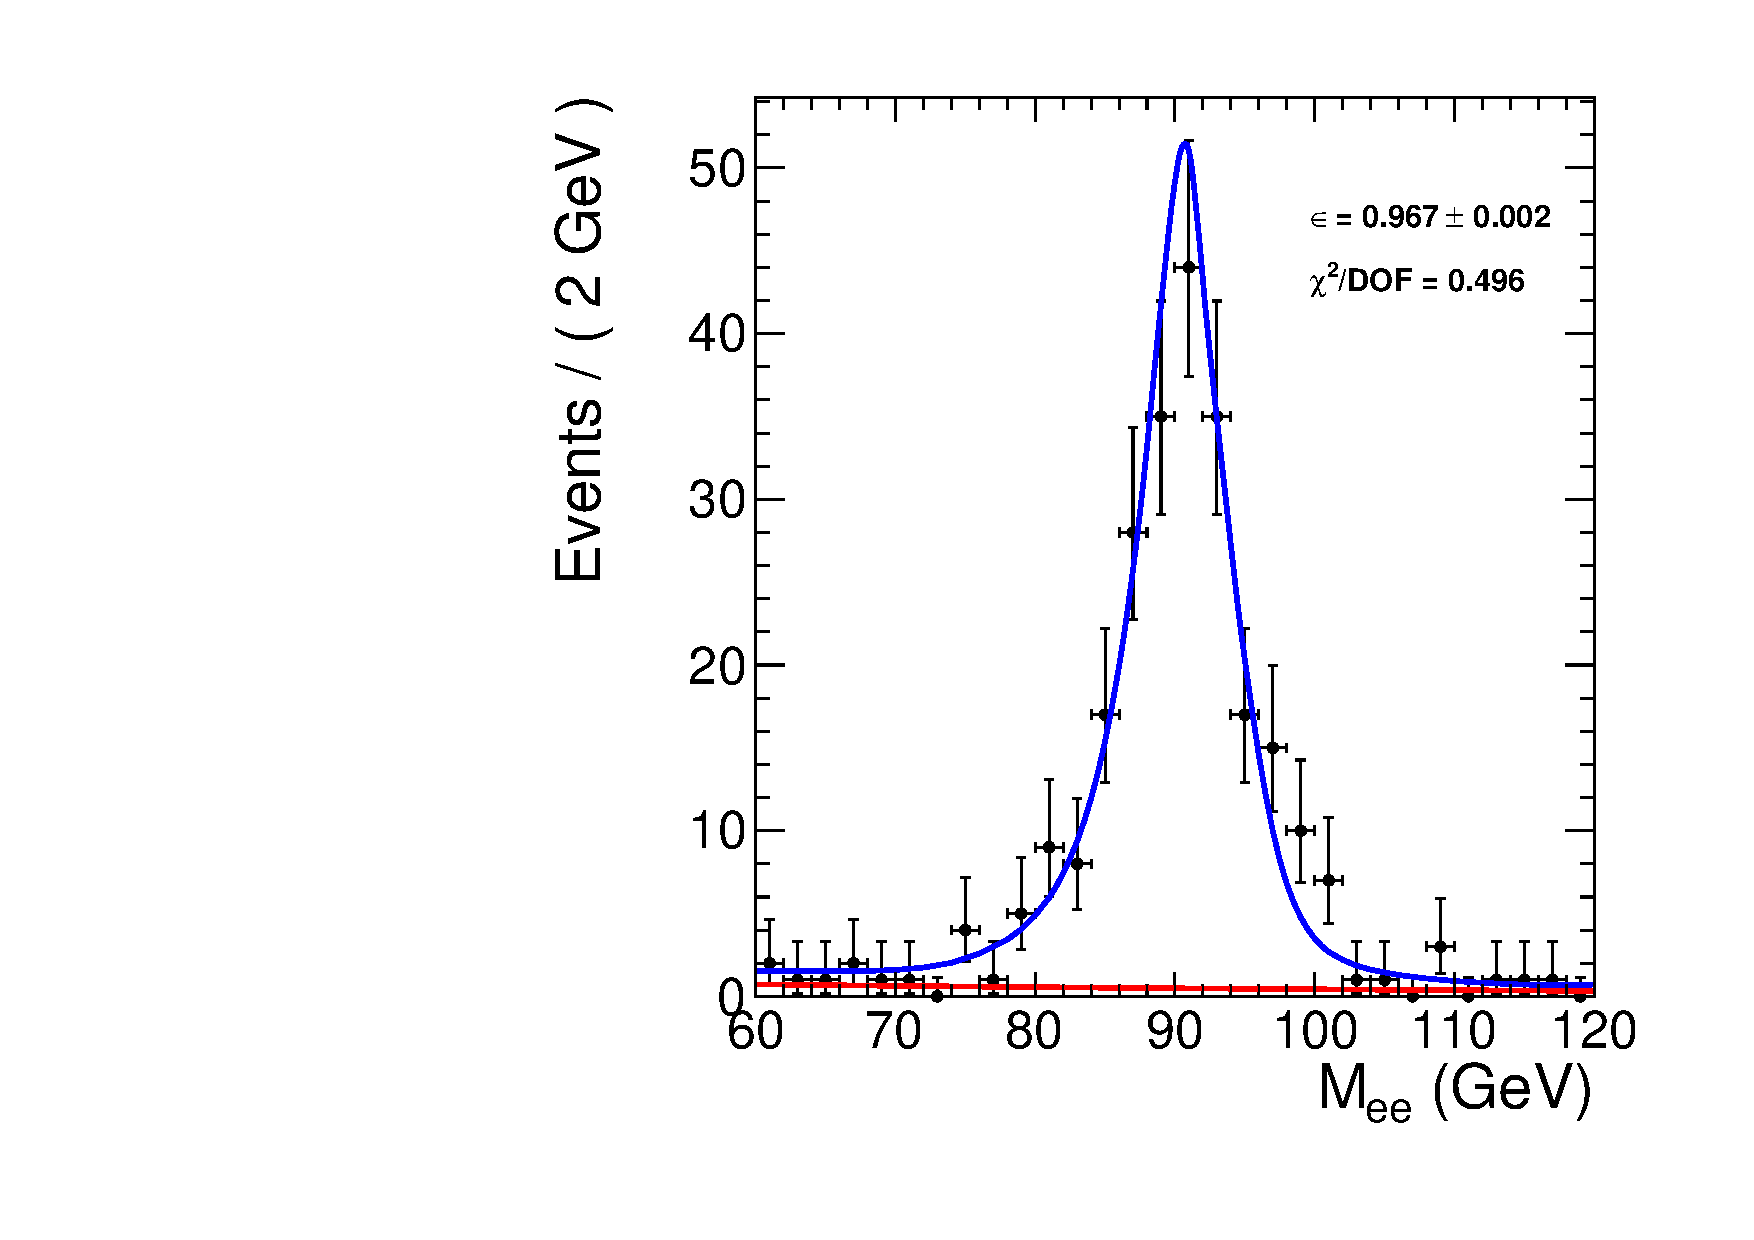
\includegraphics[width=0.49\textwidth]{tpHistos_GSF_ee_minus_pass.pdf}}
    \subfigure[]{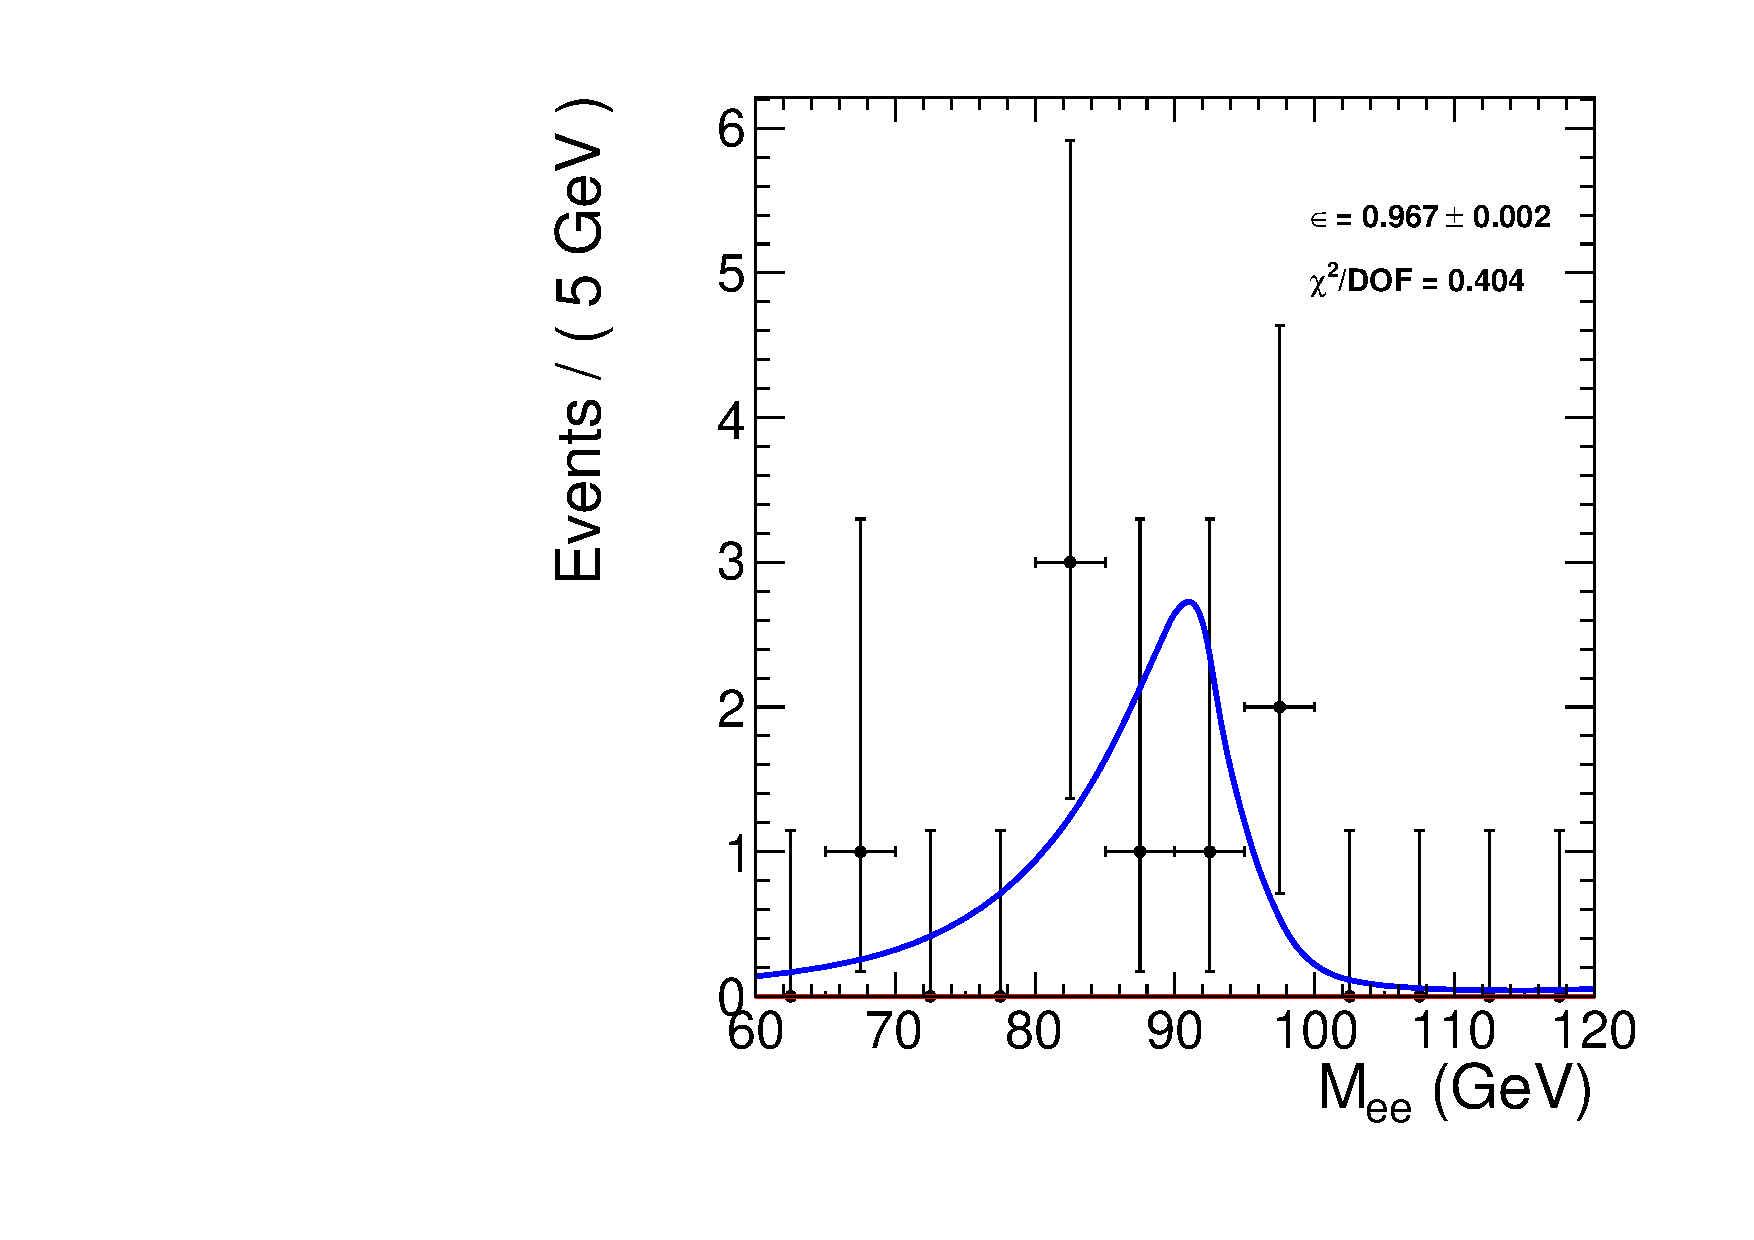
\includegraphics[width=0.49\textwidth]{tpHistos_GSF_ee_minus_fail.pdf}}
    \caption{The passing (a) and failing (b) fits for the SC$\to$Reco step in the Ecal Endcap for electrons.
             The data is in black, background fit in red, and signal+background fit in blue.}
  \end{center}
\end{figure}

\begin{figure}[htb]
  \begin{center}
    \subfigure[]{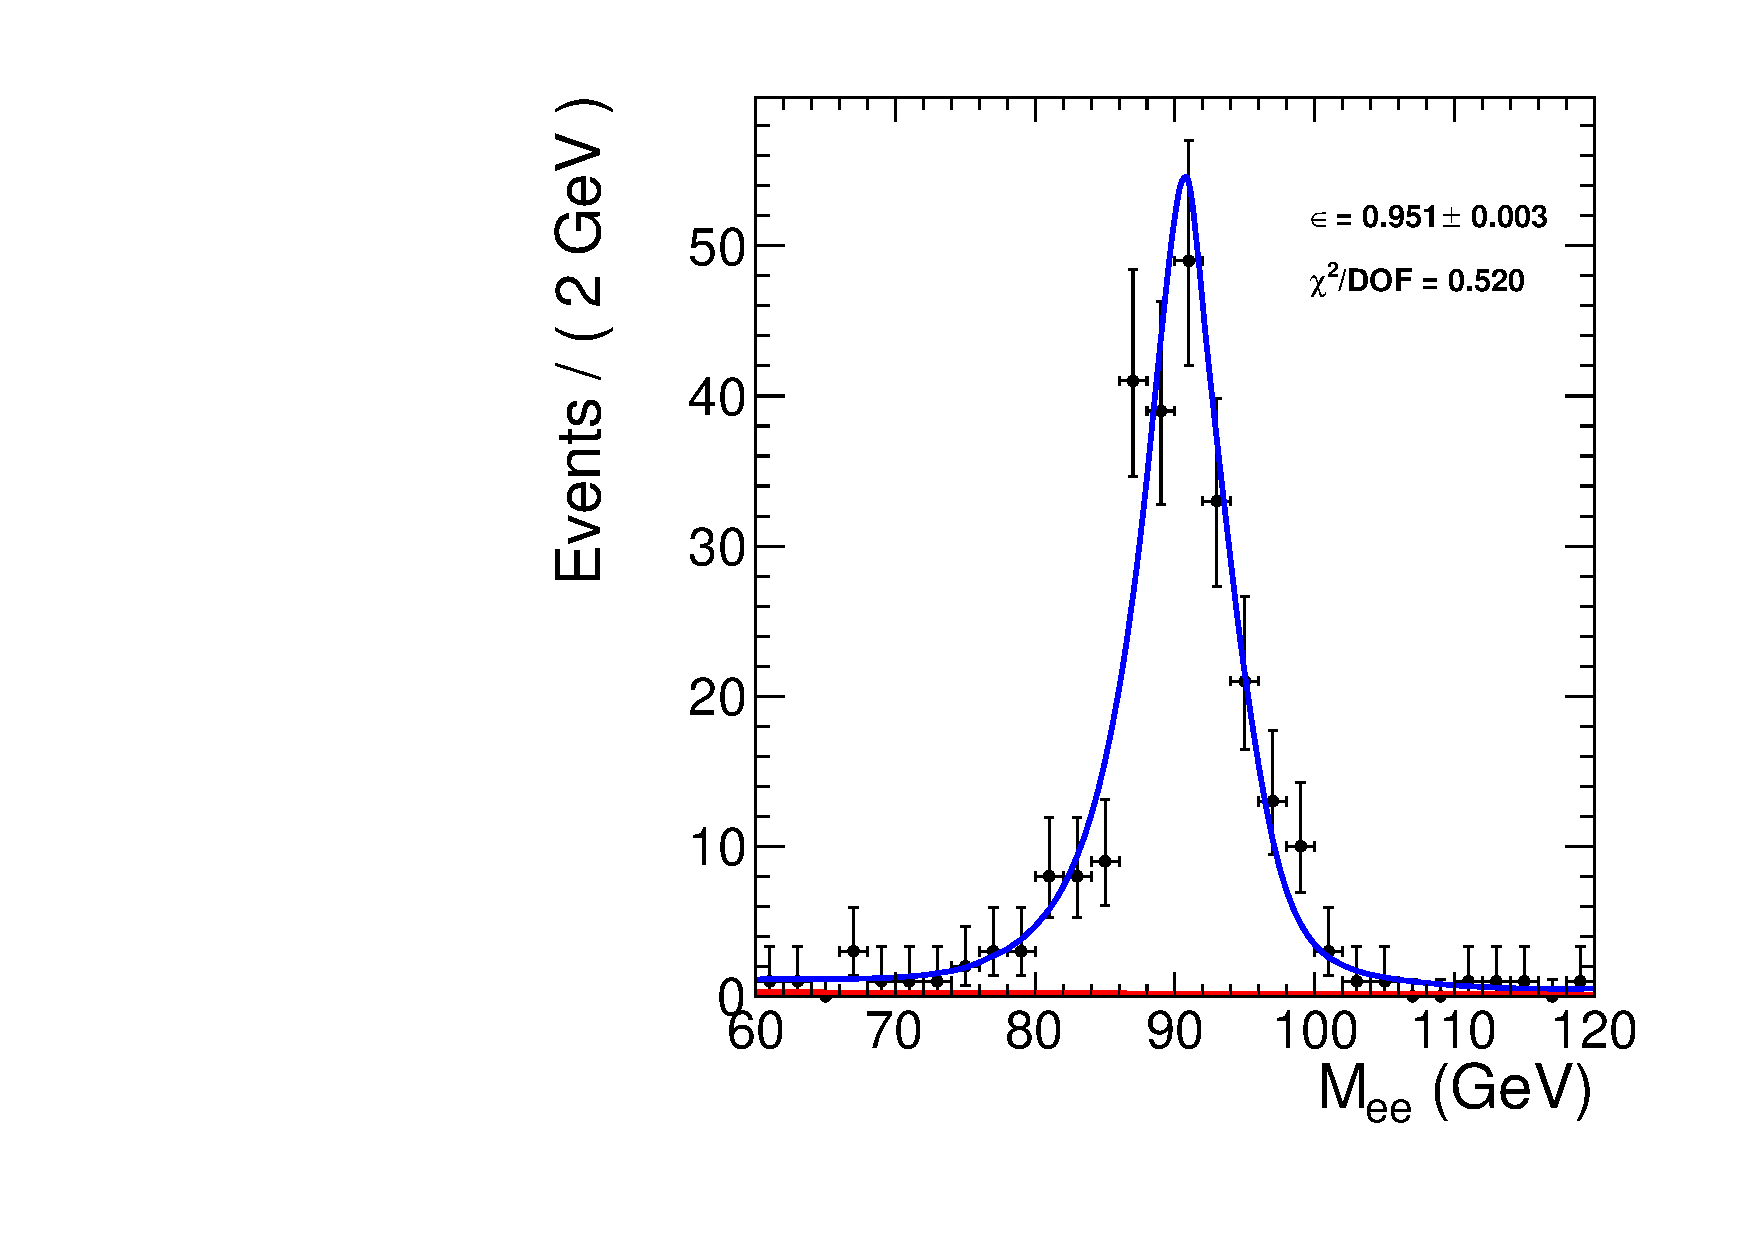
\includegraphics[width=0.49\textwidth]{tpHistos_GSF_ee_plus_pass.pdf}}
    \subfigure[]{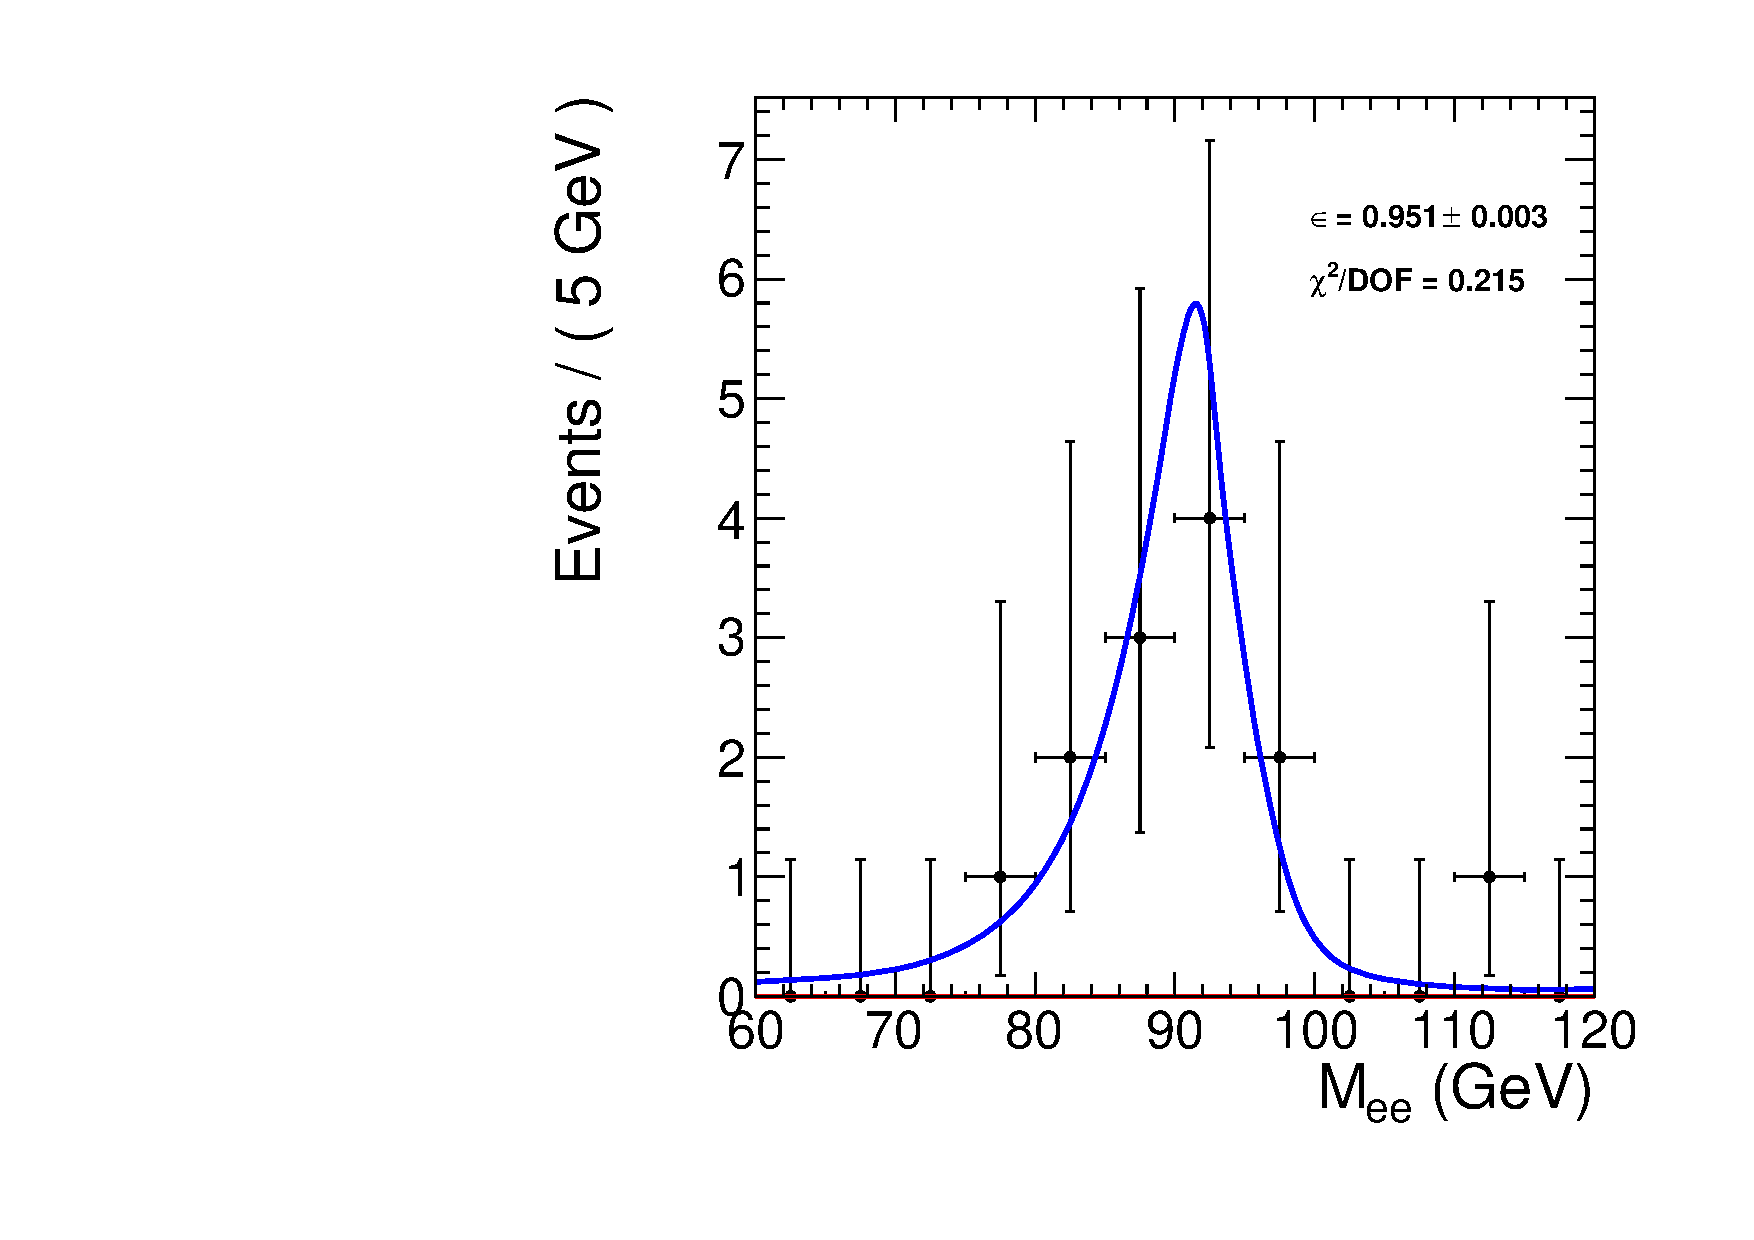
\includegraphics[width=0.49\textwidth]{tpHistos_GSF_ee_plus_fail.pdf}}
    \caption{The passing (a) and failing (b) fits for the SC$\to$Reco step in the Ecal Endcap for positrons.
             The data is in black, background fit in red, and signal+background fit in blue.}
  \end{center}
\end{figure}



%reco->wp80
\begin{figure}[htb]
  \begin{center}
    \subfigure[]{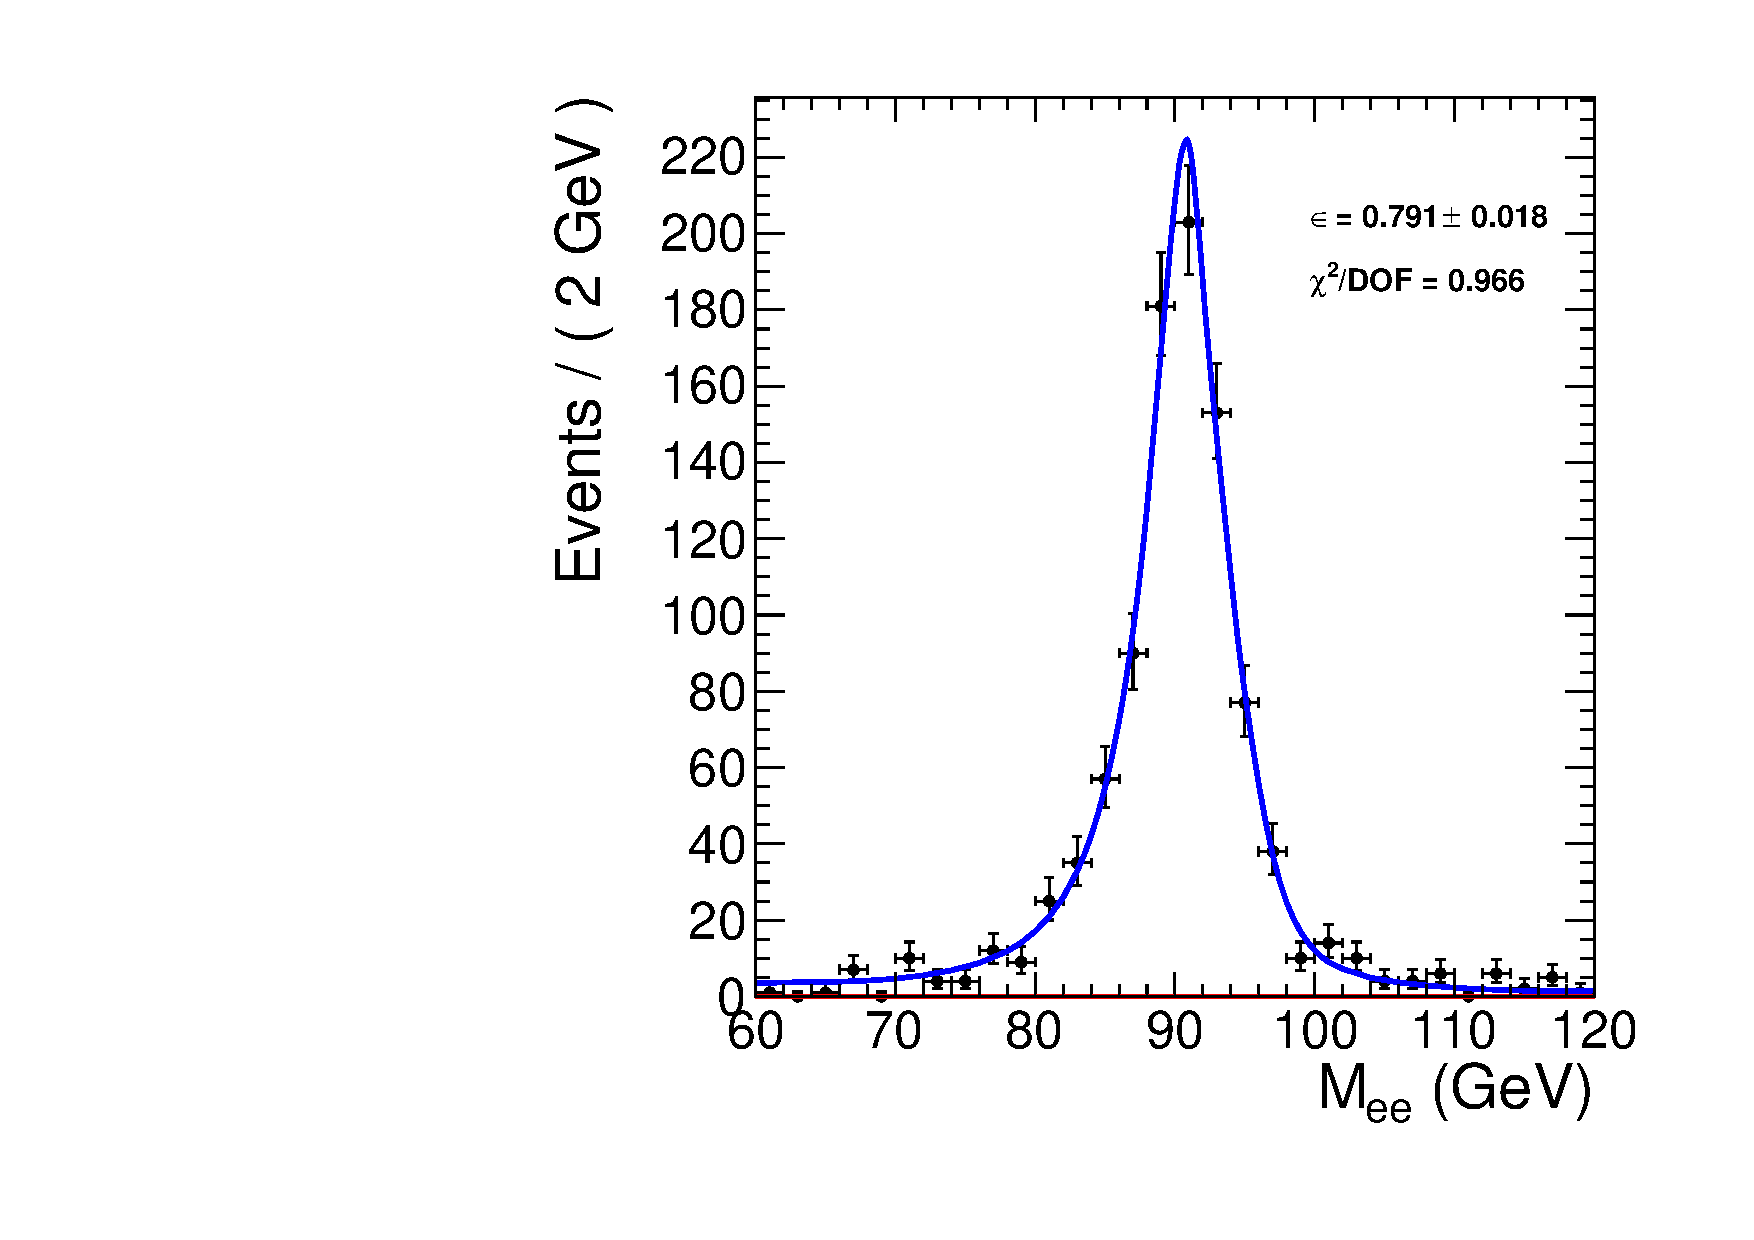
\includegraphics[width=0.49\textwidth]{tpHistos_ID80_eb_pass.pdf}}
    \subfigure[]{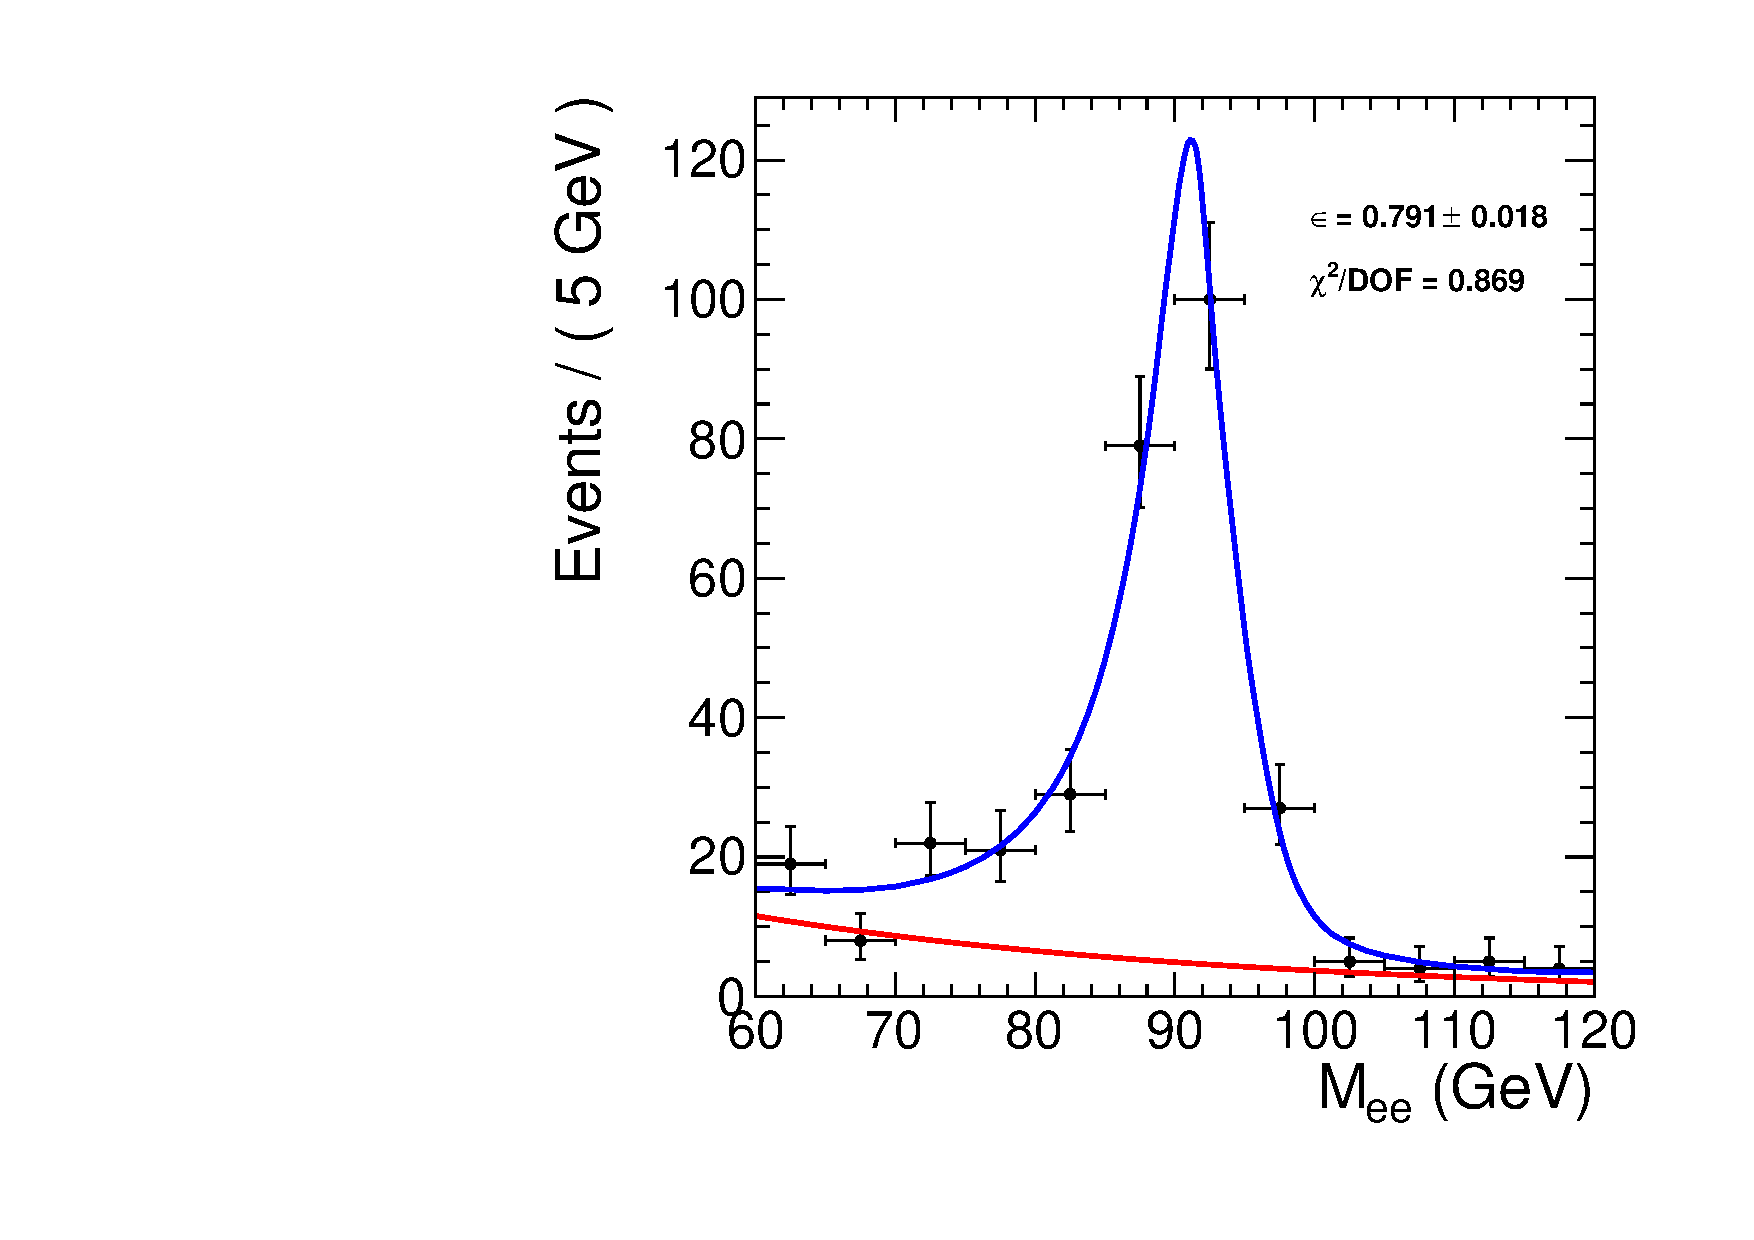
\includegraphics[width=0.49\textwidth]{tpHistos_ID80_eb_fail.pdf}}
    \caption{The passing (a) and failing (b) fits for the Reco$\to$WP80 step in the Ecal Barrel.
             The data is in black, background fit in red, and signal+background fit in blue.}
  \end{center}
\end{figure}

\begin{figure}[htb]
  \begin{center}
    \subfigure[]{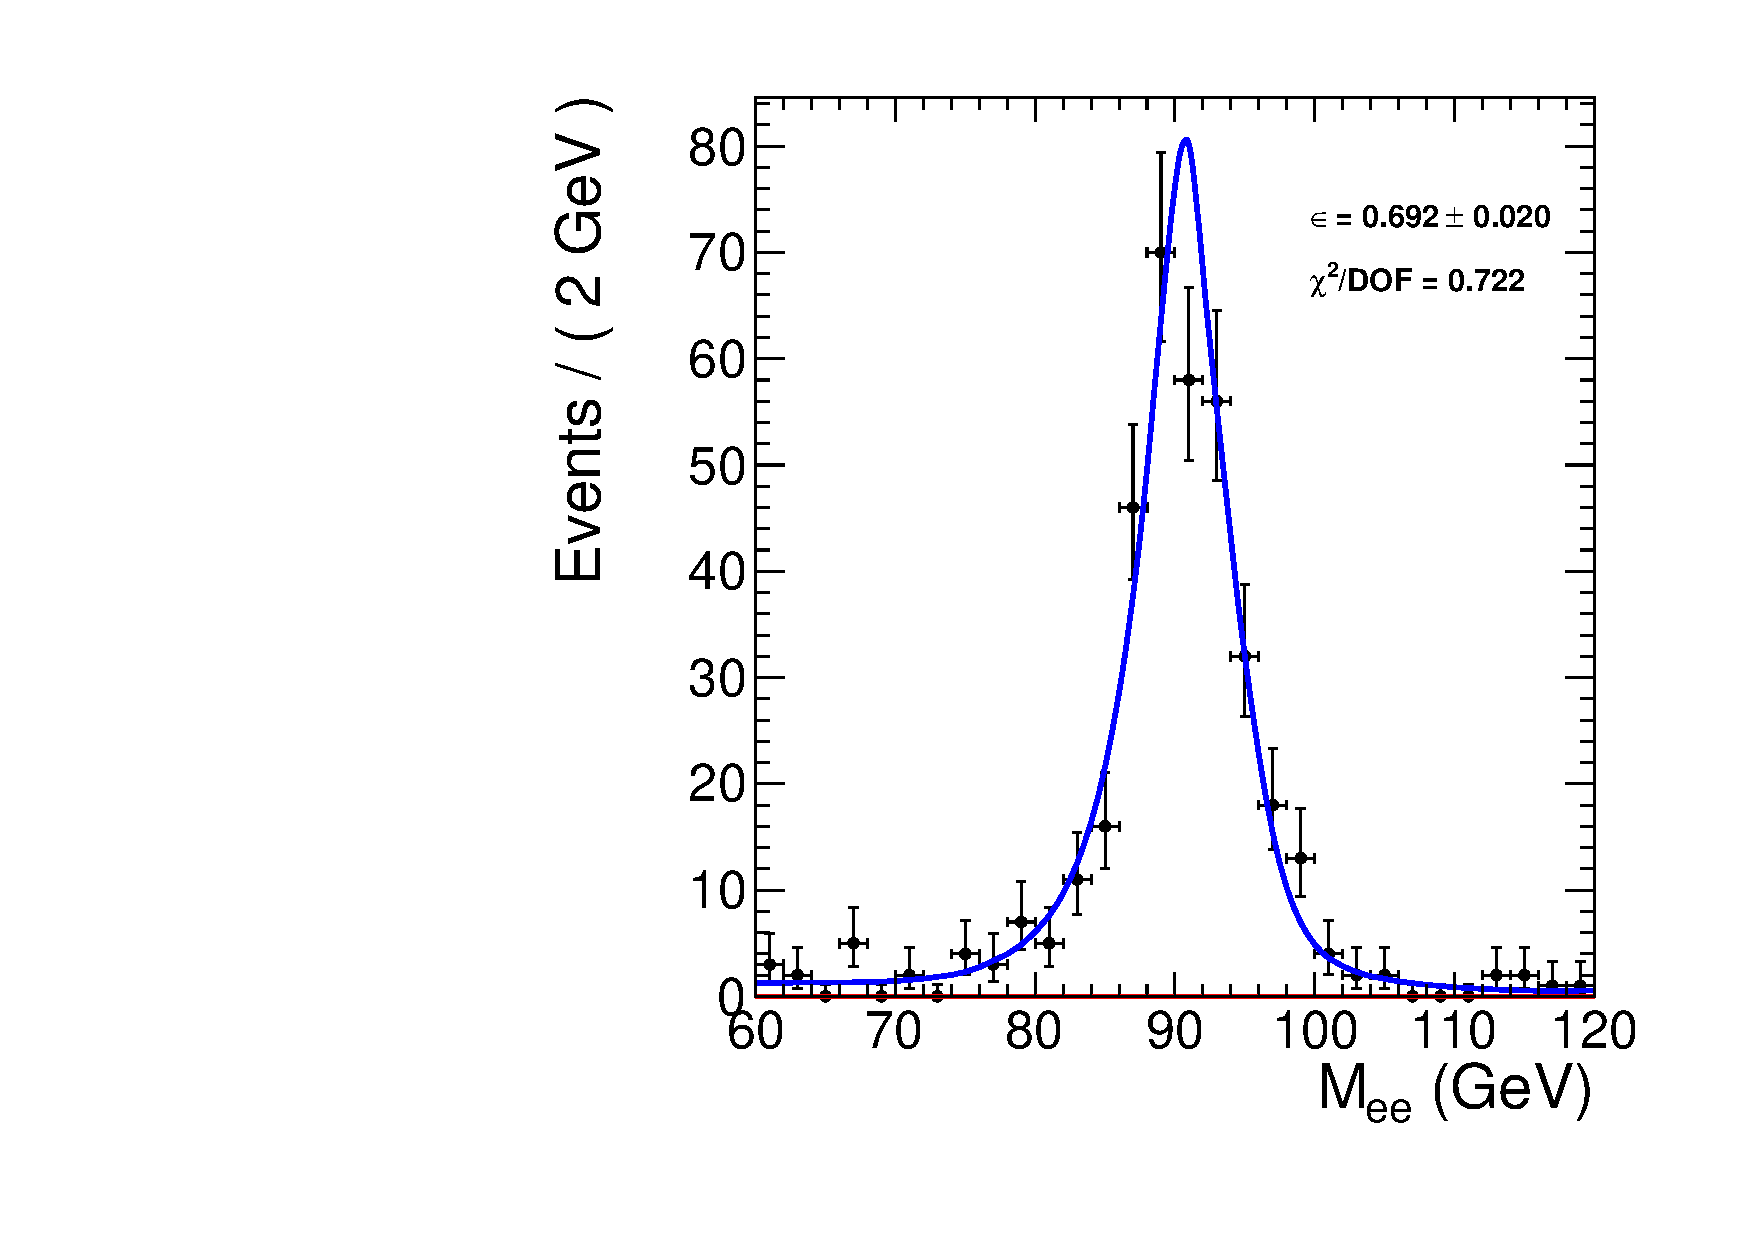
\includegraphics[width=0.49\textwidth]{tpHistos_ID80_ee_pass.pdf}}
    \subfigure[]{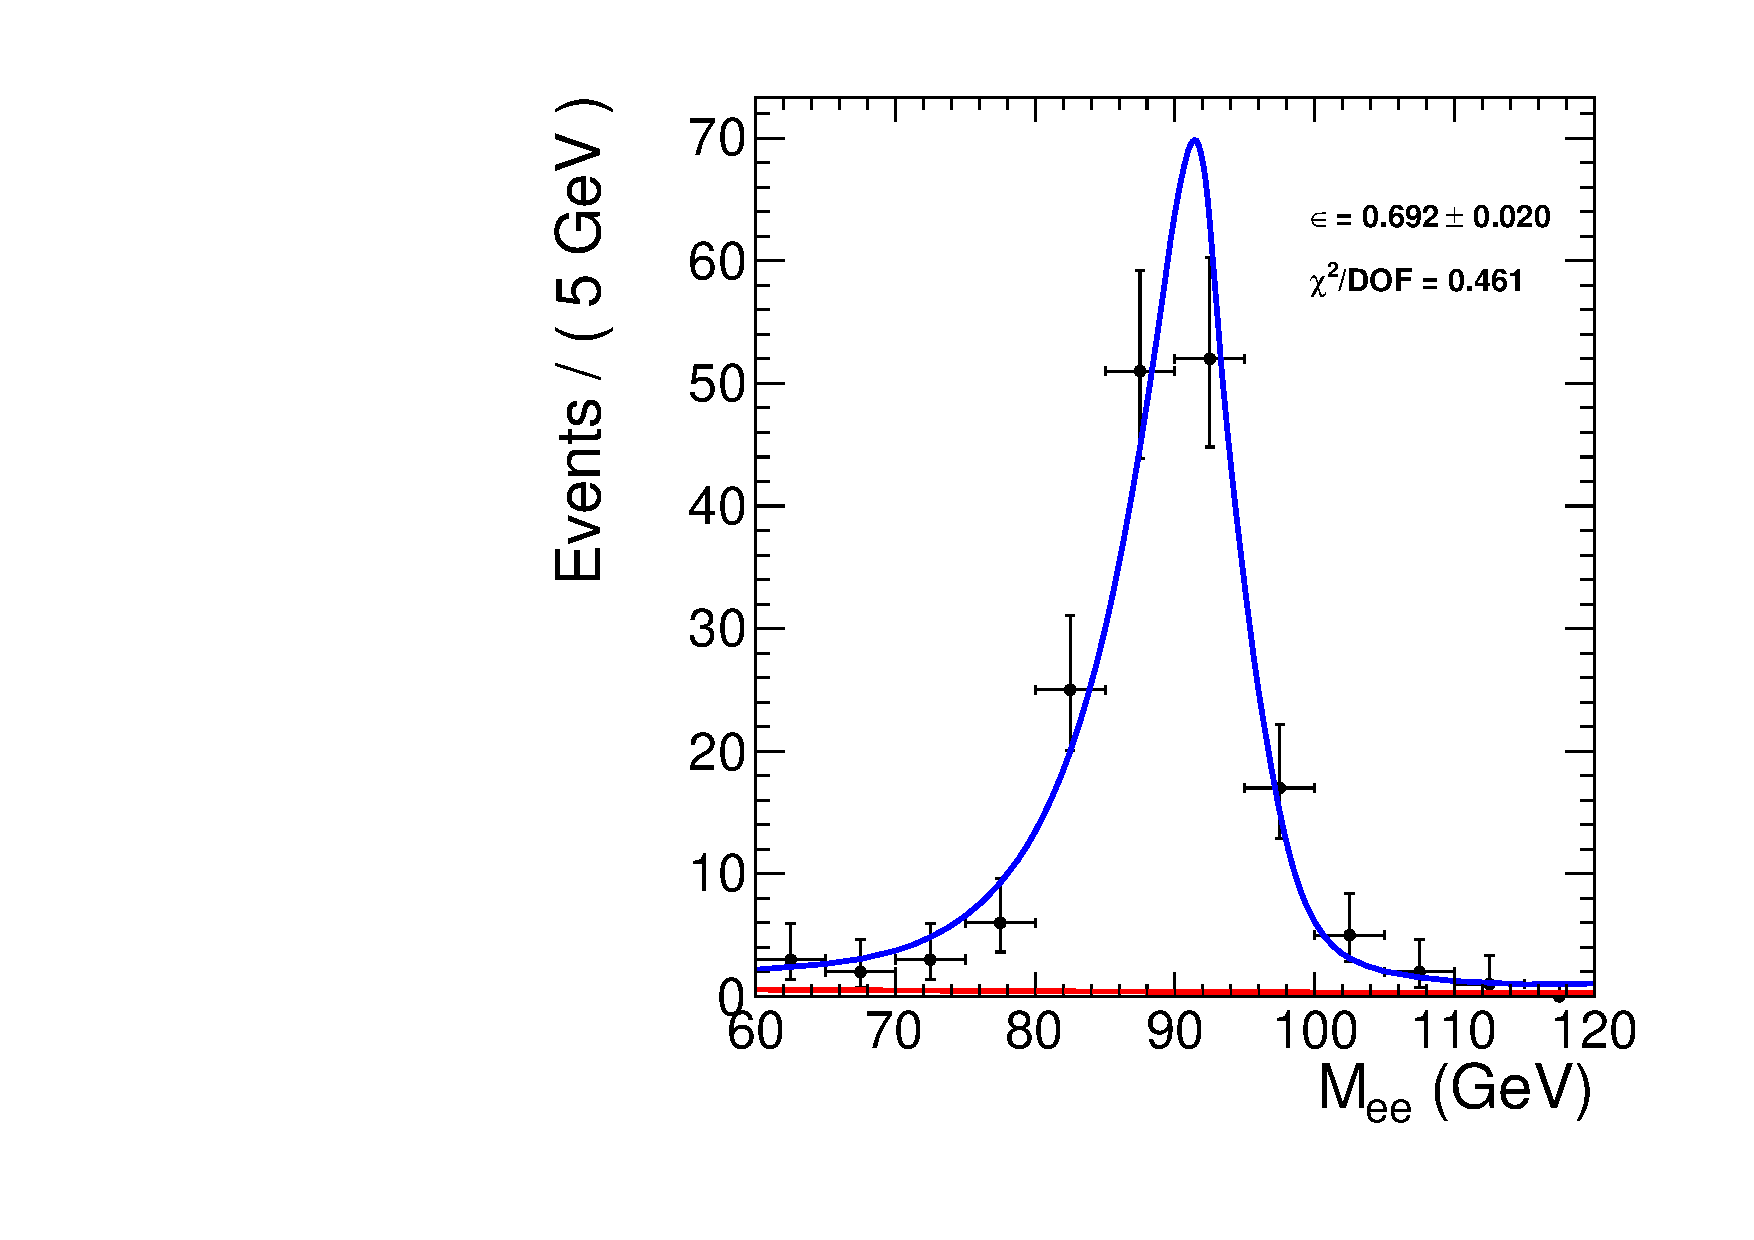
\includegraphics[width=0.49\textwidth]{tpHistos_ID80_ee_fail.pdf}}
    \caption{The passing (a) and failing (b) fits for the Reco$\to$WP80 step in the Ecal Endcap.  
             The data is in black, background fit in red, and signal+background fit in blue.}
  \end{center}
\end{figure}

\begin{figure}[htb]
  \begin{center}
    \subfigure[]{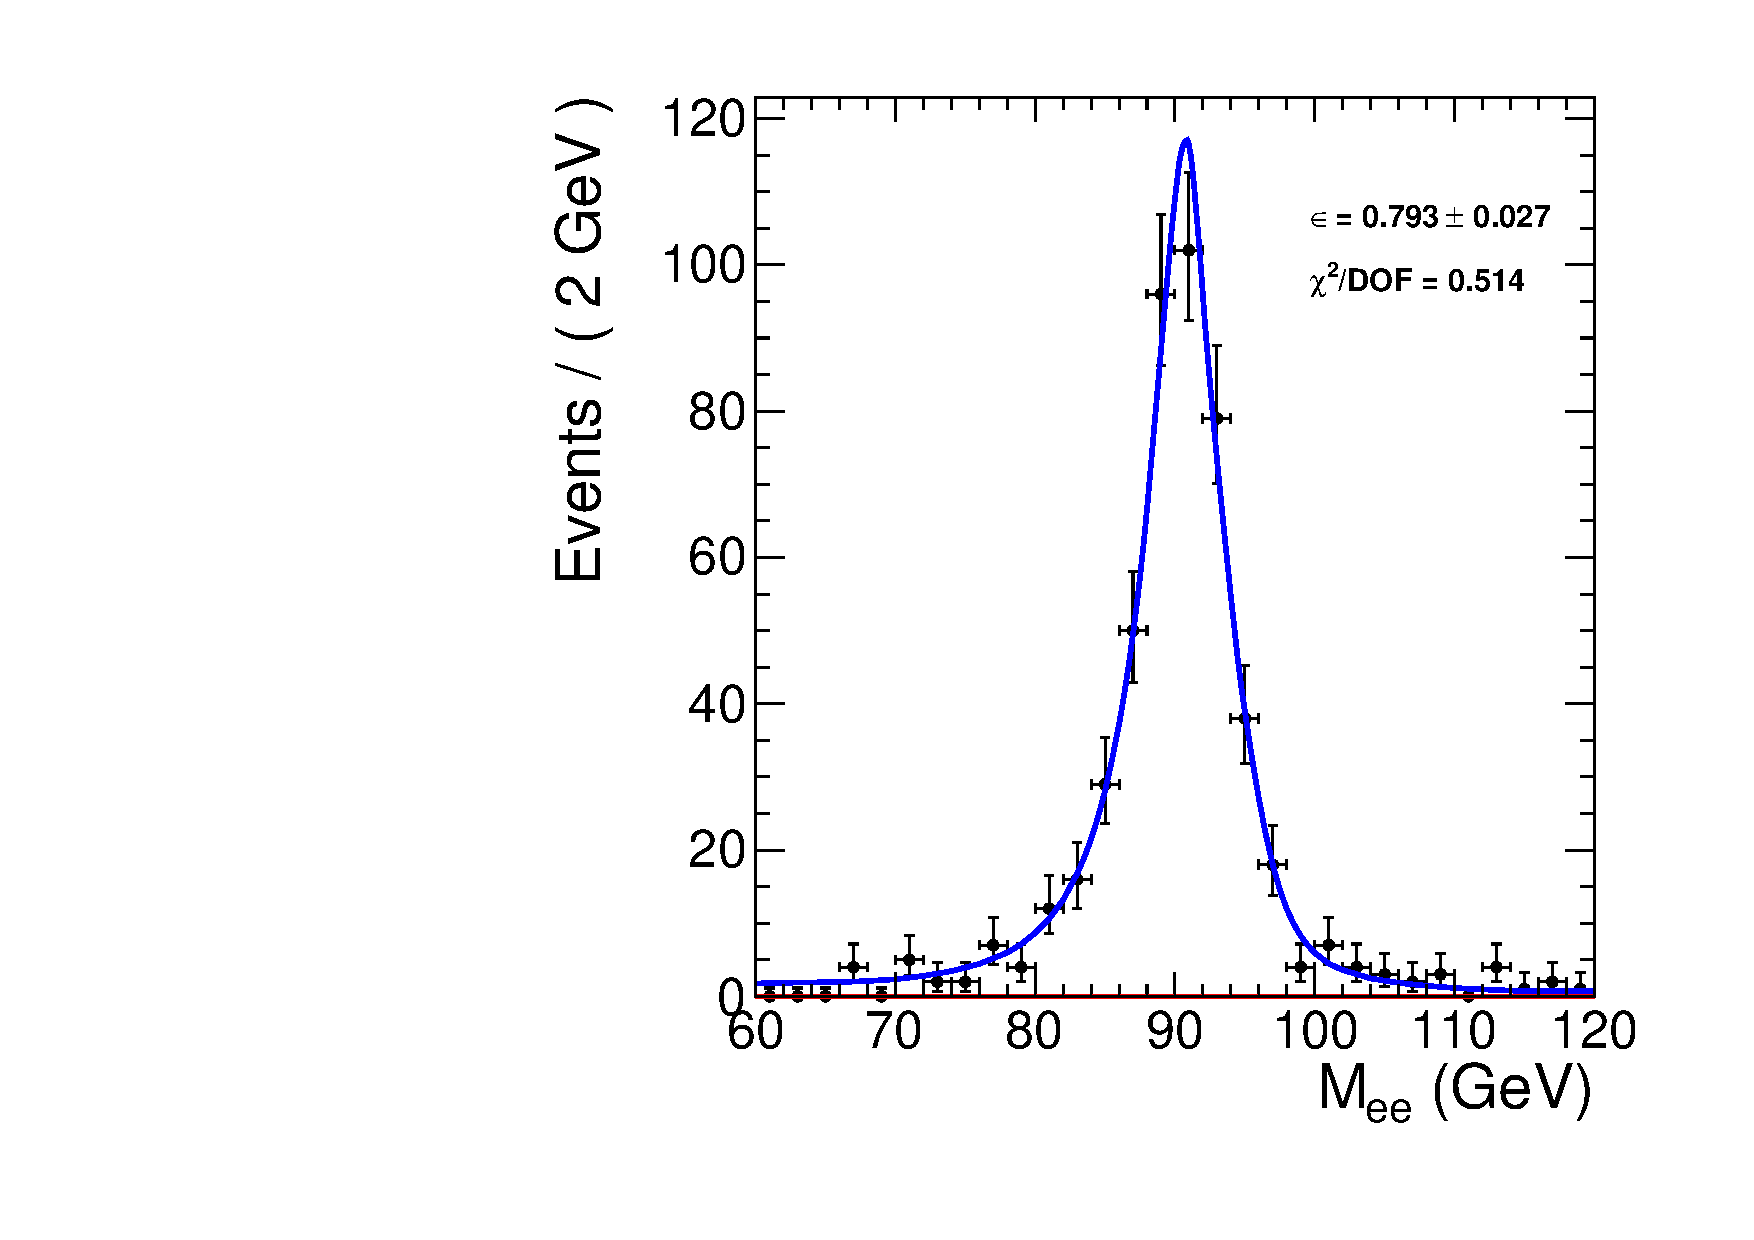
\includegraphics[width=0.49\textwidth]{tpHistos_ID80_eb_minus_pass.pdf}}
    \subfigure[]{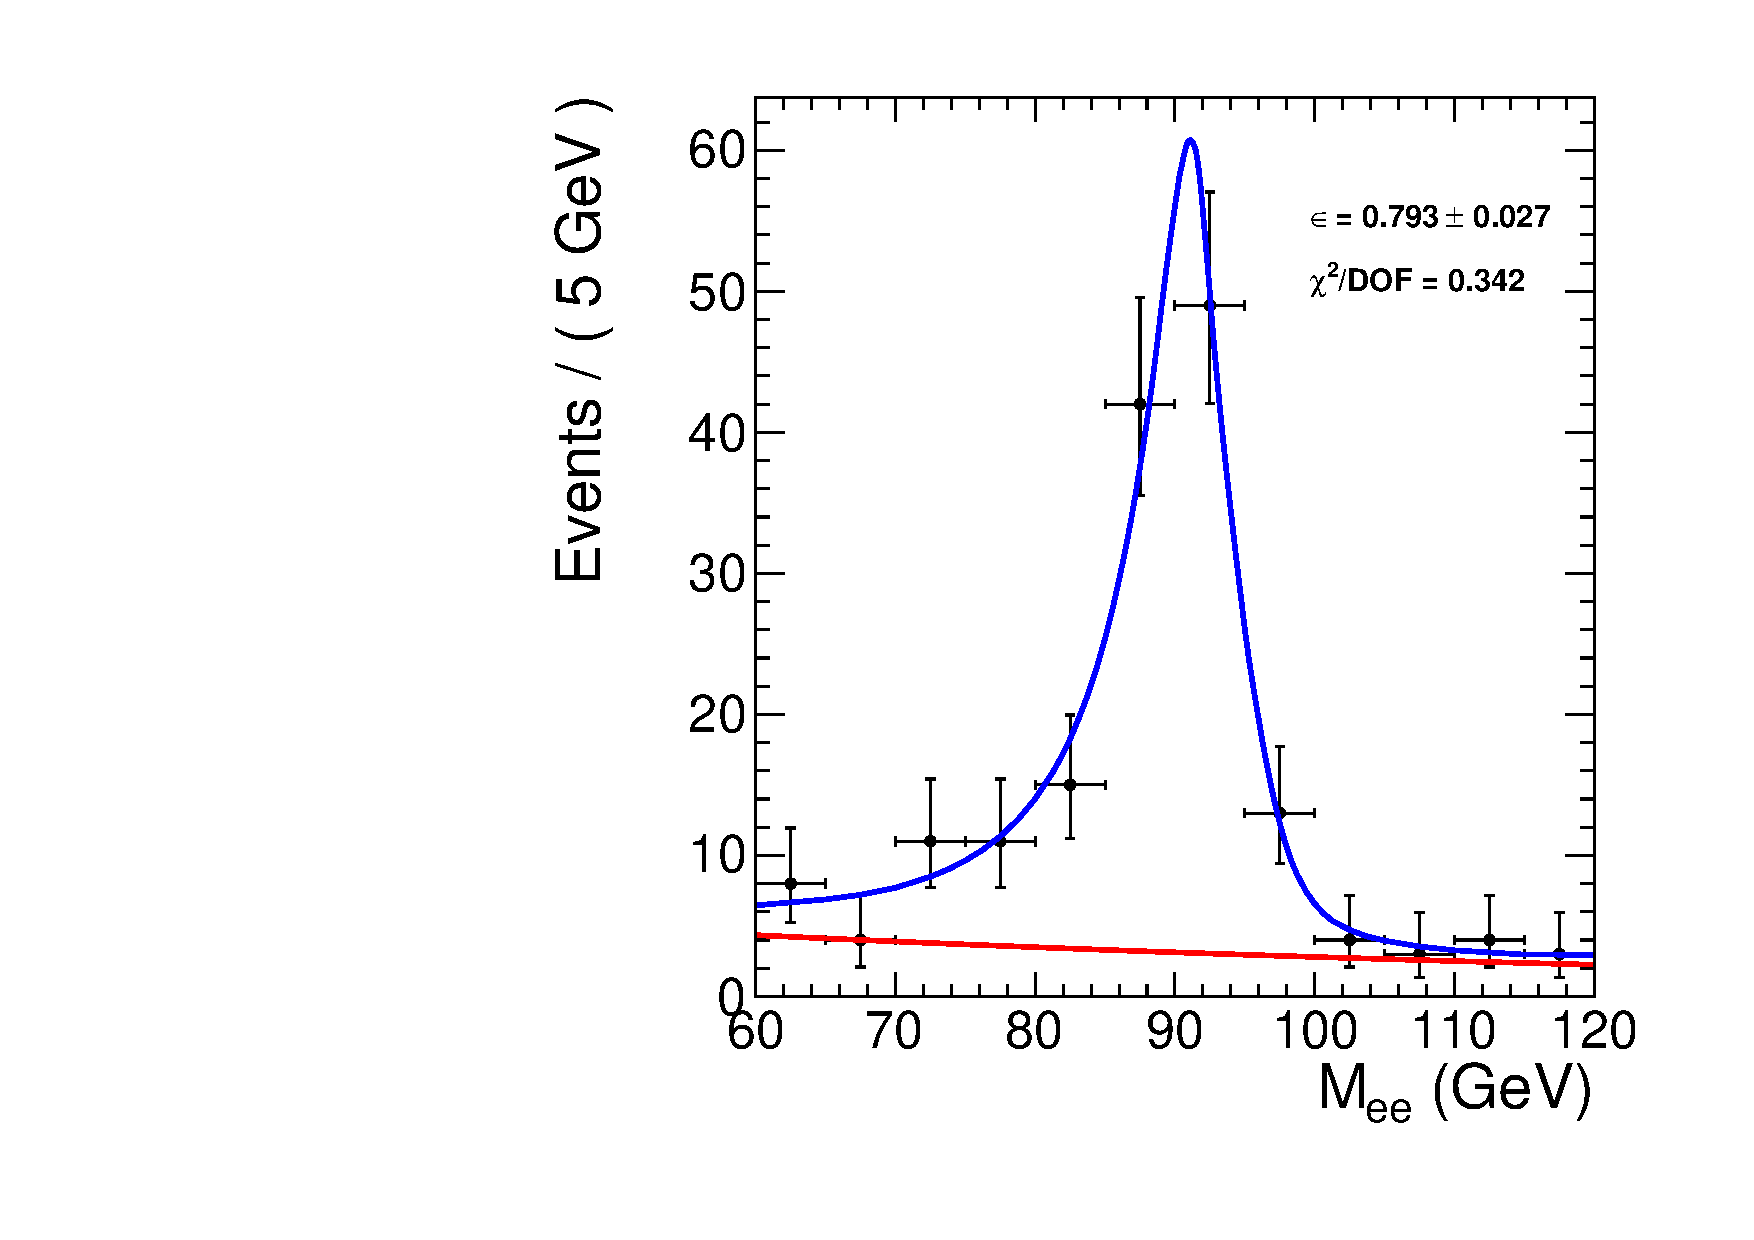
\includegraphics[width=0.49\textwidth]{tpHistos_ID80_eb_minus_fail.pdf}}
    \caption{The passing (a) and failing (b) fits for the Reco$\to$WP80 step in the Ecal Barrel for electrons.
             The data is in black, background fit in red, and signal+background fit in blue.}
  \end{center}
\end{figure}

\begin{figure}[htb]
  \begin{center}
    \subfigure[]{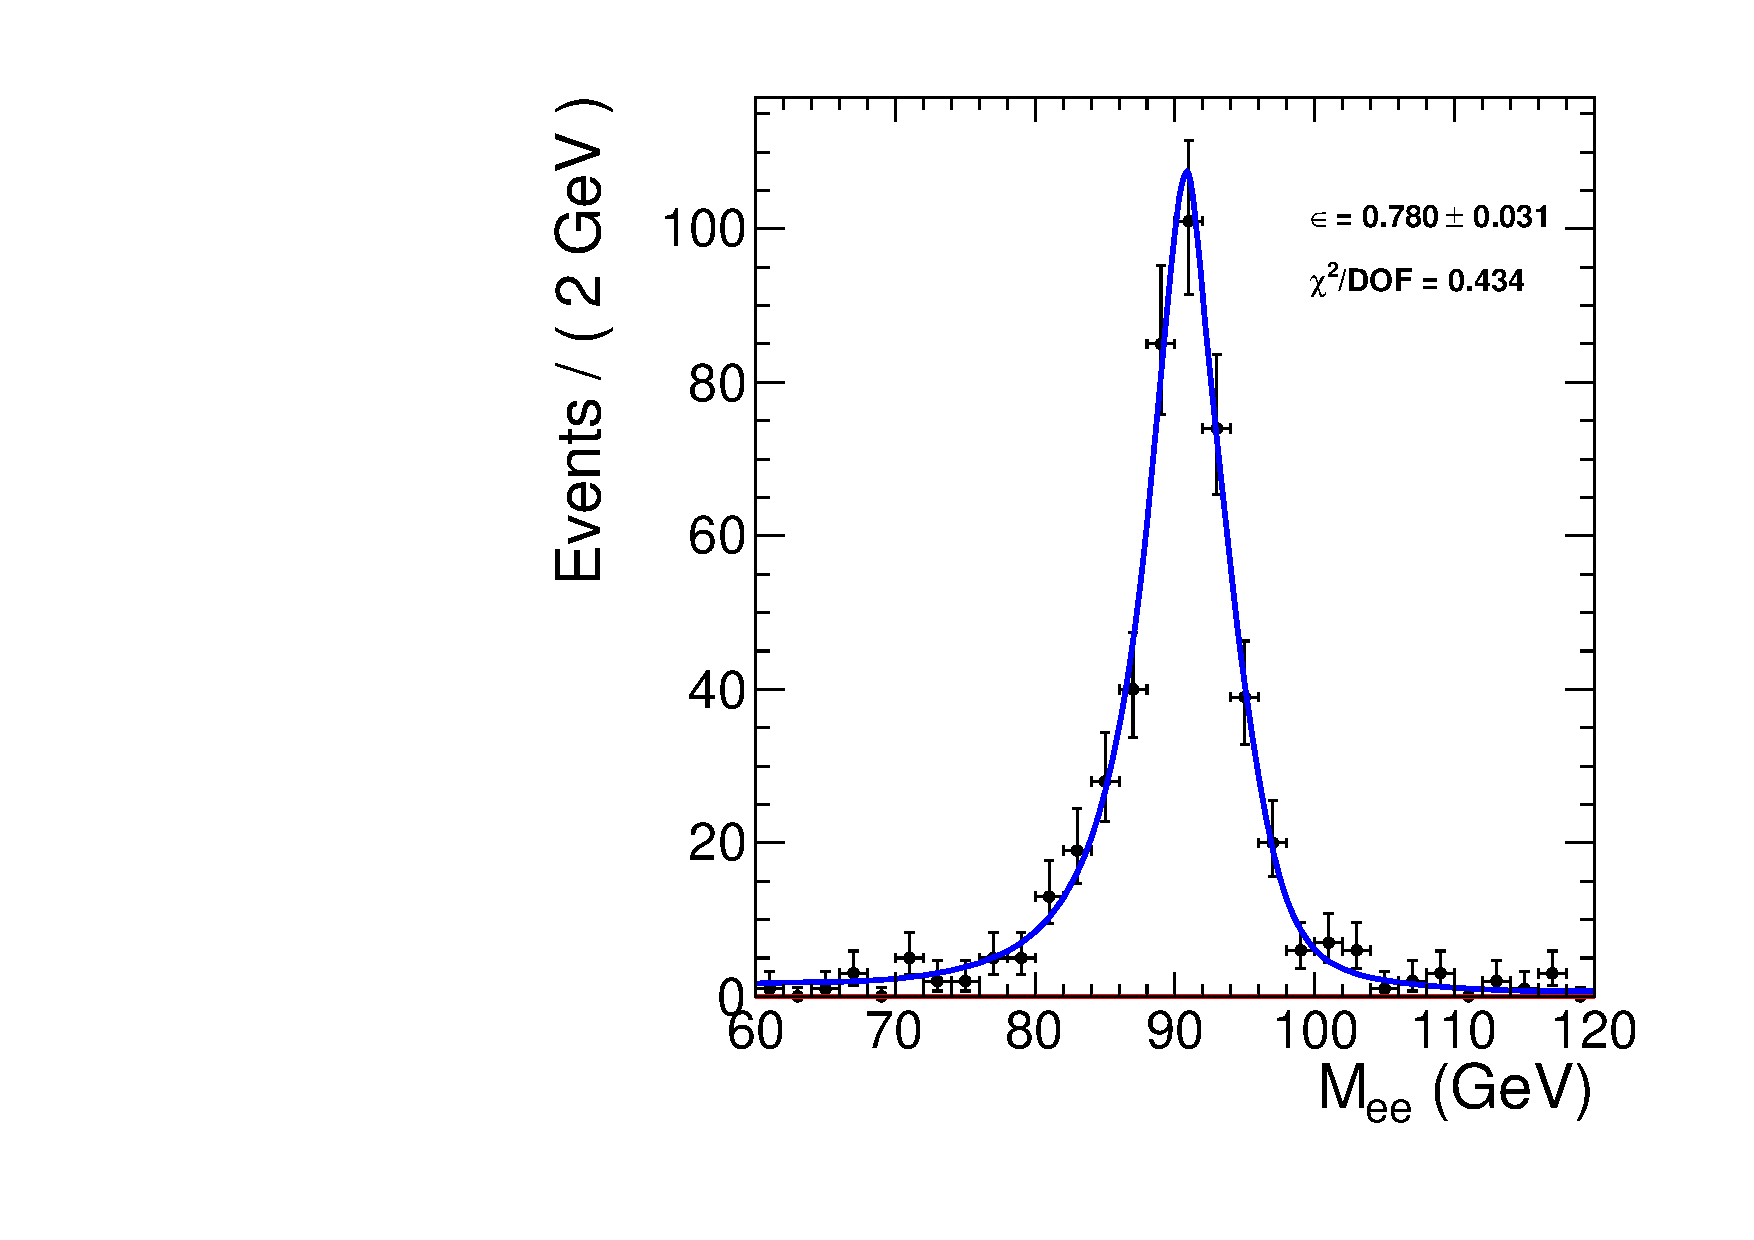
\includegraphics[width=0.49\textwidth]{tpHistos_ID80_eb_plus_pass.pdf}}
    \subfigure[]{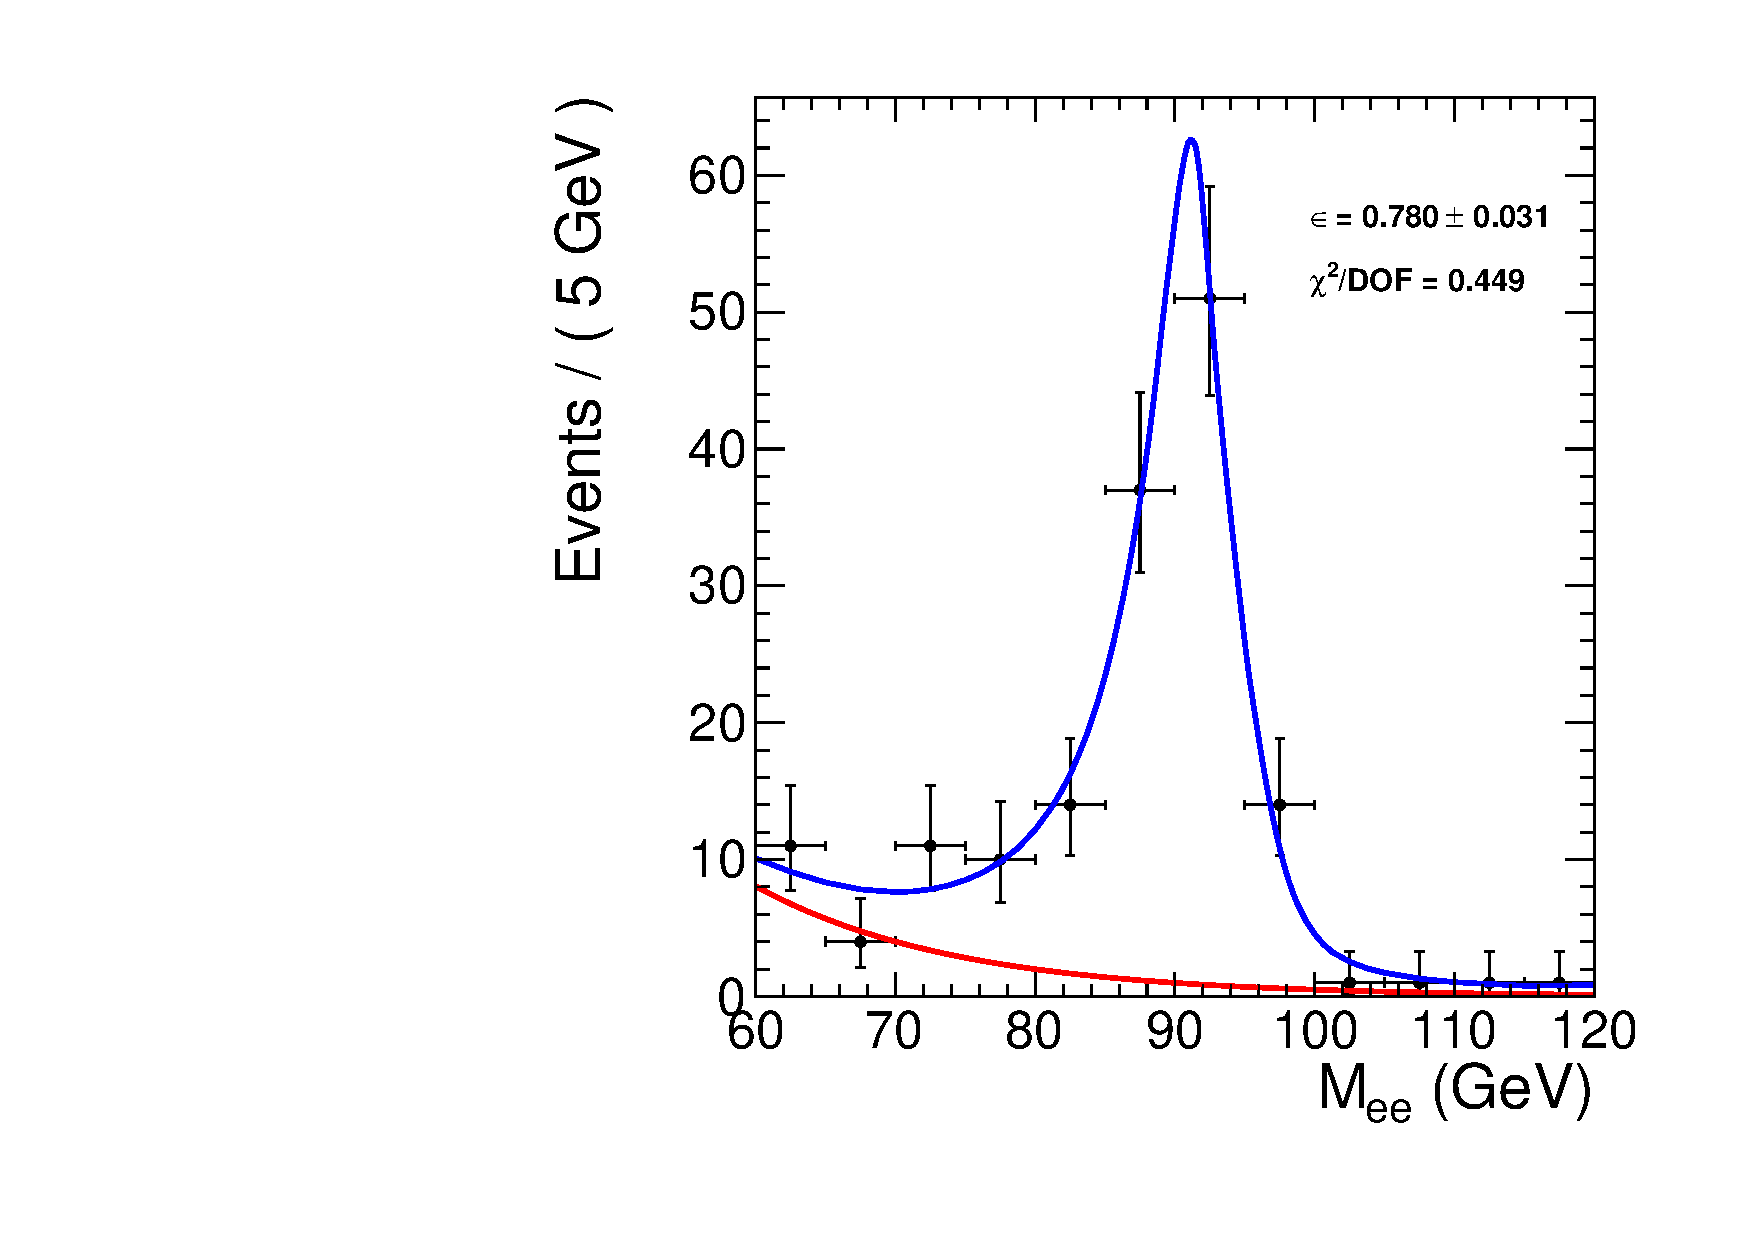
\includegraphics[width=0.49\textwidth]{tpHistos_ID80_eb_plus_fail.pdf}}
    \caption{The passing (a) and failing (b) fits for the Reco$\to$WP80 step in the Ecal Barrel for positrons.
             The data is in black, background fit in red, and signal+background fit in blue.}
  \end{center}
\end{figure}

\begin{figure}[htb]
  \begin{center}
    \subfigure[]{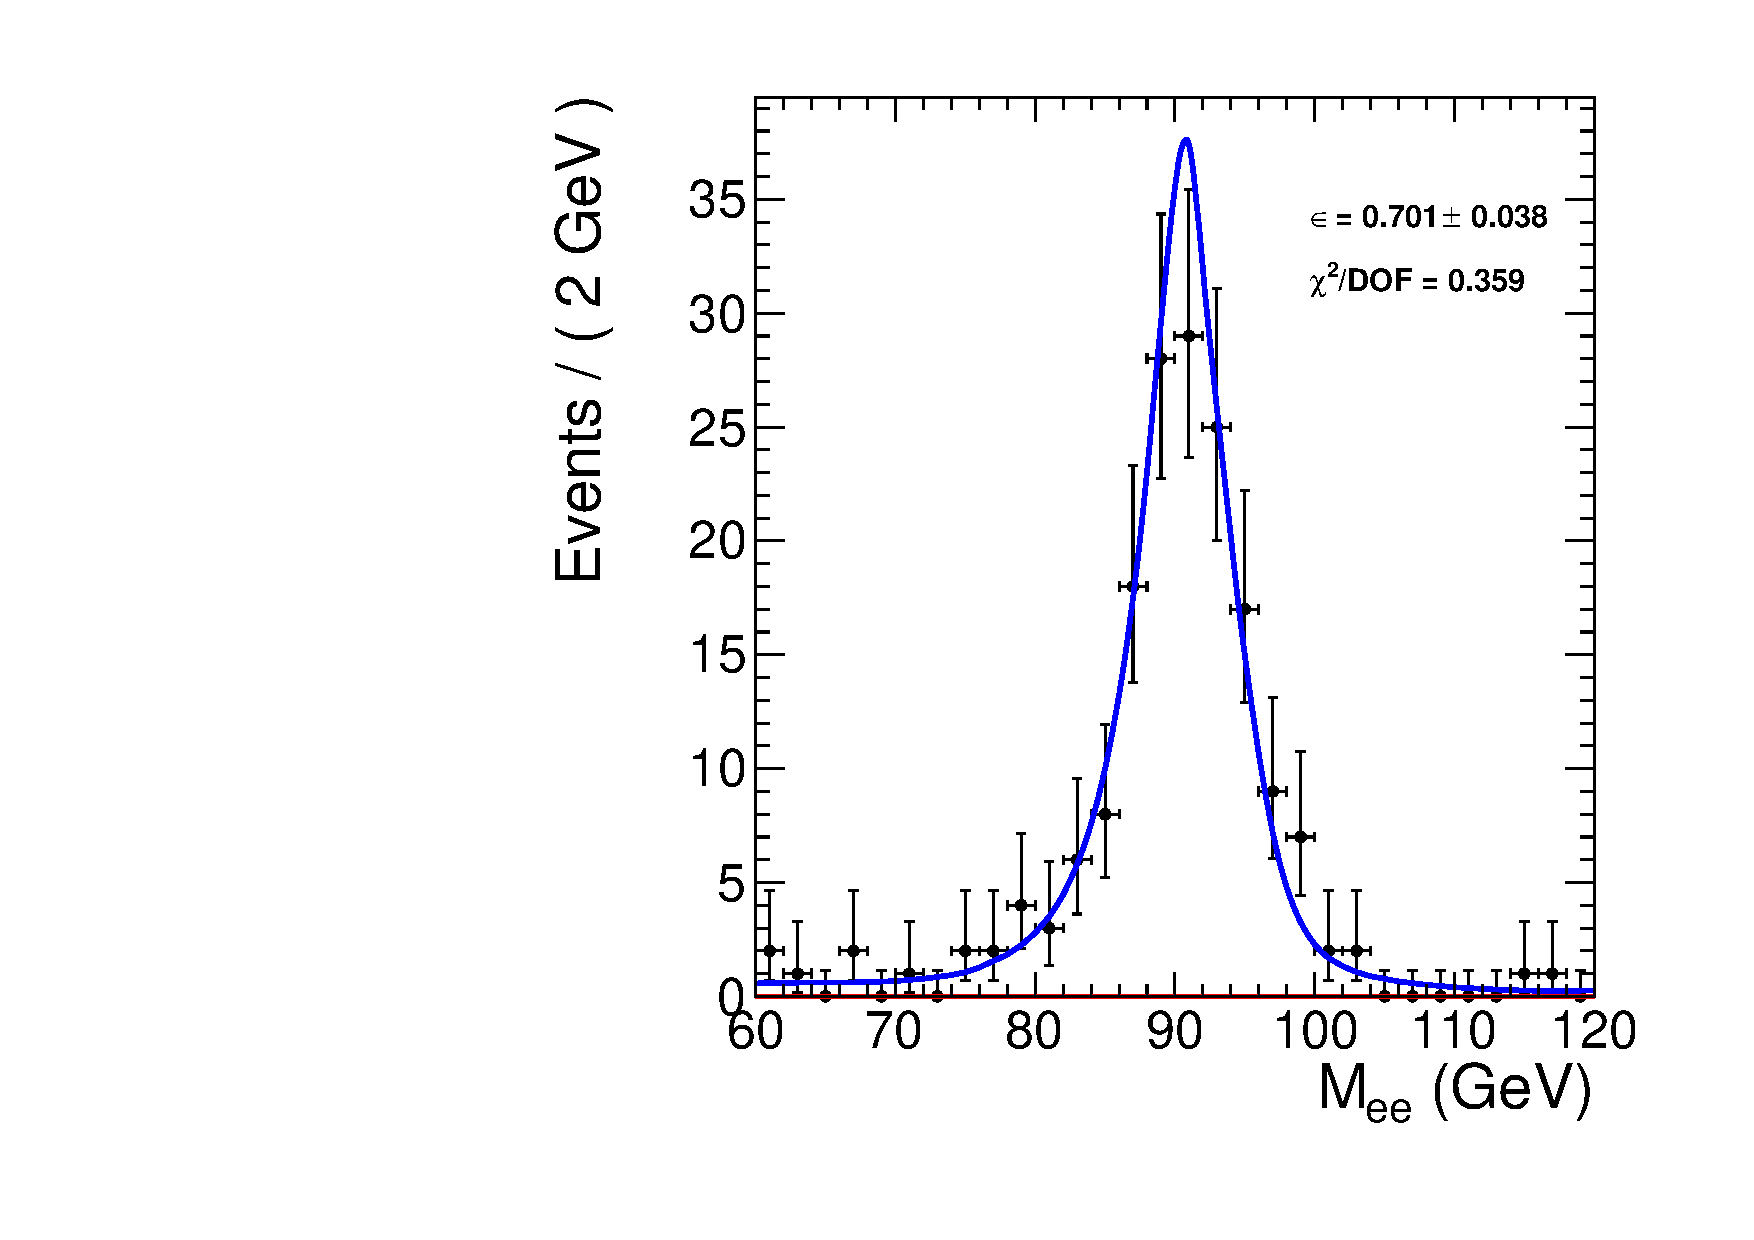
\includegraphics[width=0.49\textwidth]{tpHistos_ID80_ee_minus_pass.pdf}}
    \subfigure[]{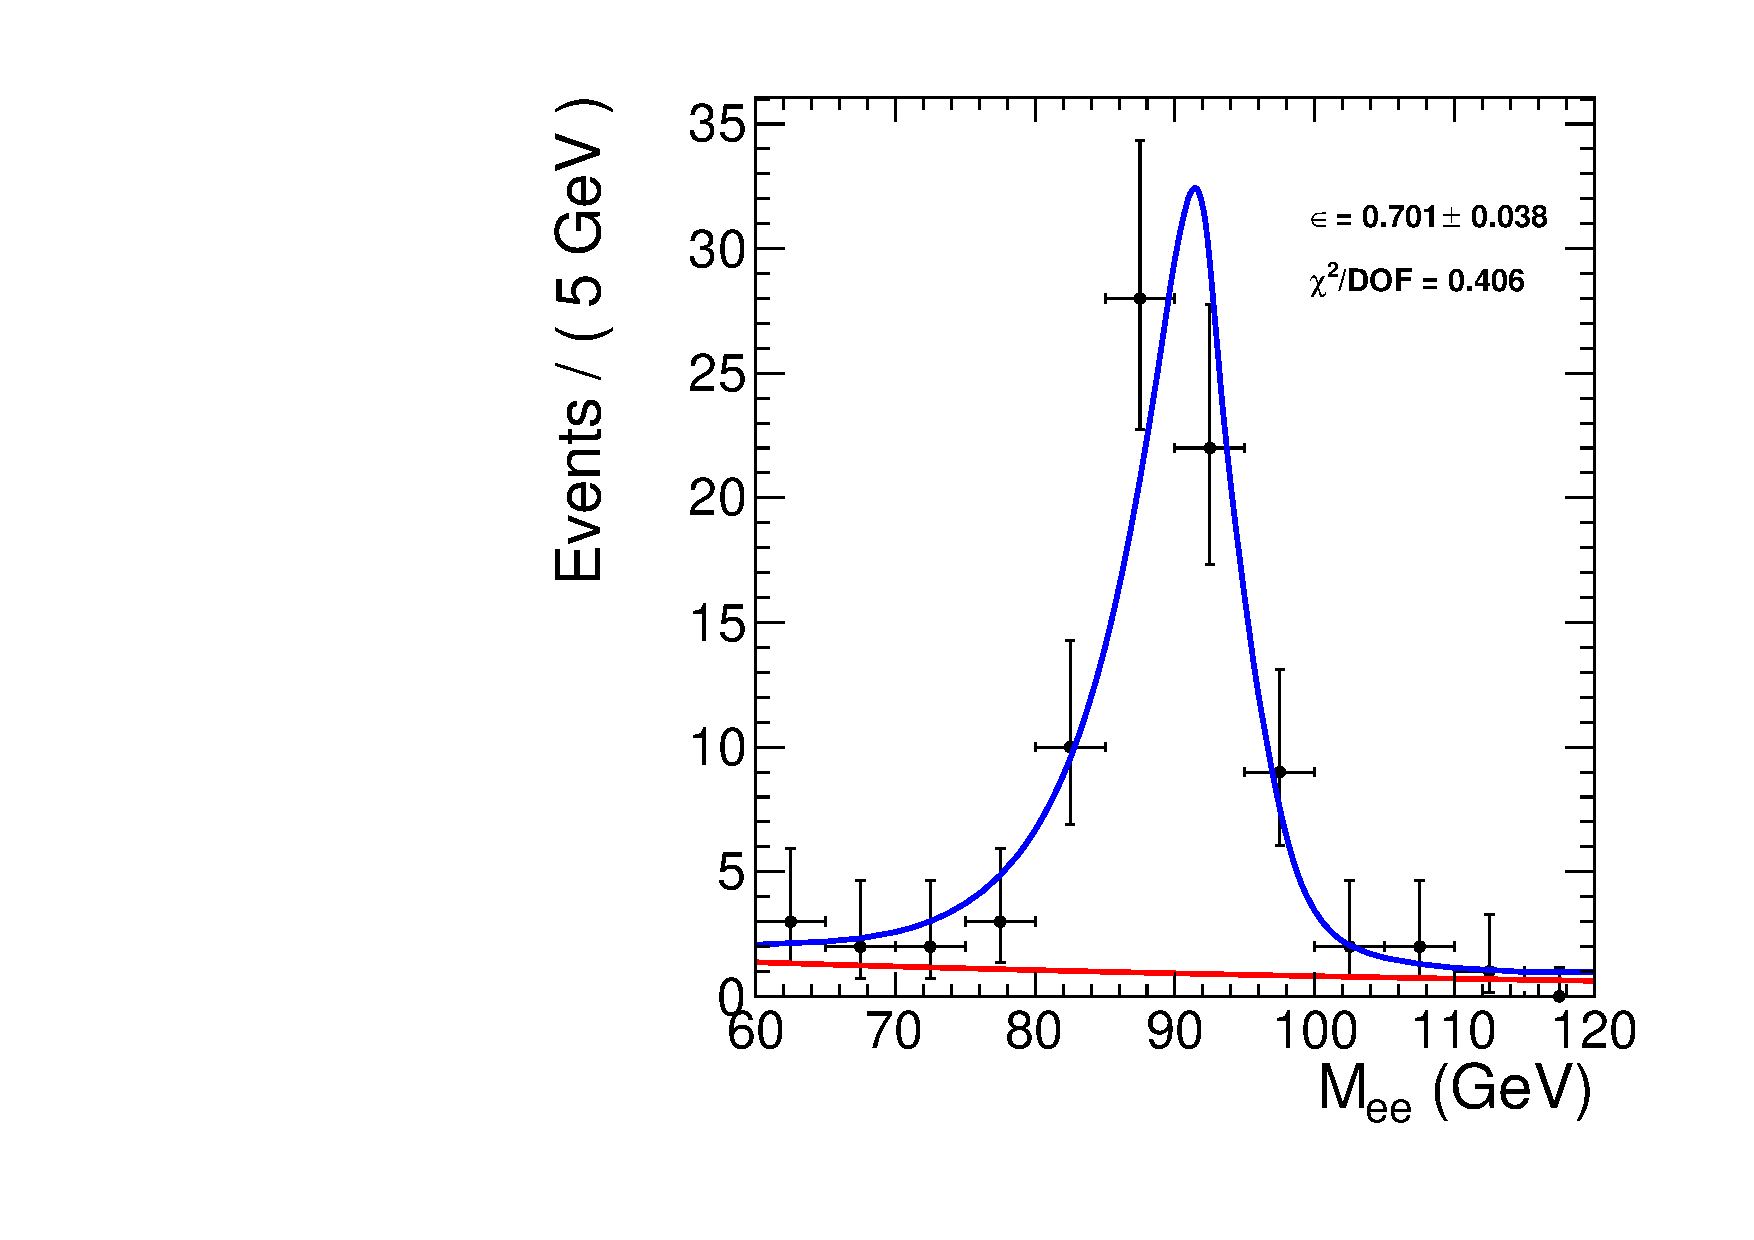
\includegraphics[width=0.49\textwidth]{tpHistos_ID80_ee_minus_fail.pdf}}
    \caption{The passing (a) and failing (b) fits for the Reco$\to$WP80 step in the Ecal Endcap for electrons.
             The data is in black, background fit in red, and signal+background fit in blue.}
  \end{center}
\end{figure}

\begin{figure}[htb]
  \begin{center}
    \subfigure[]{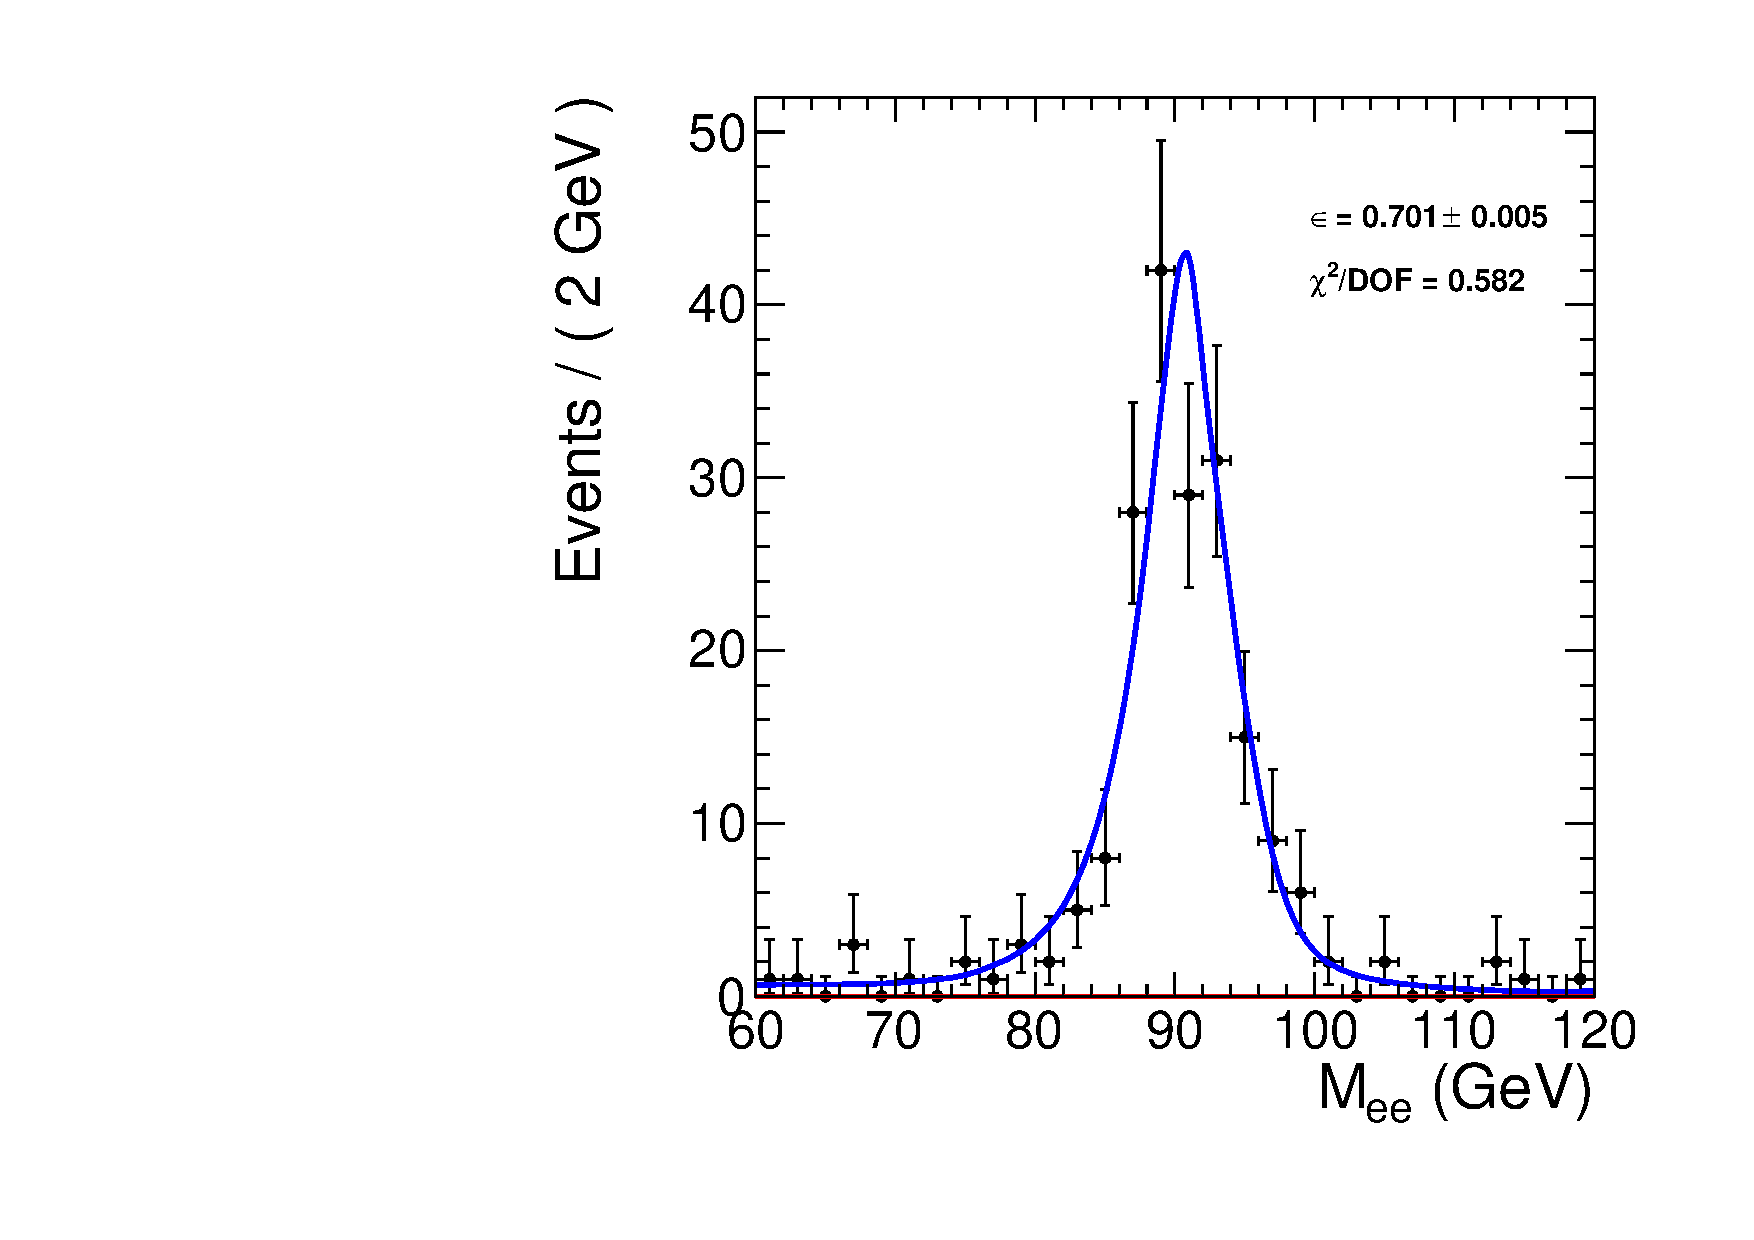
\includegraphics[width=0.49\textwidth]{tpHistos_ID80_ee_plus_pass.pdf}}
    \subfigure[]{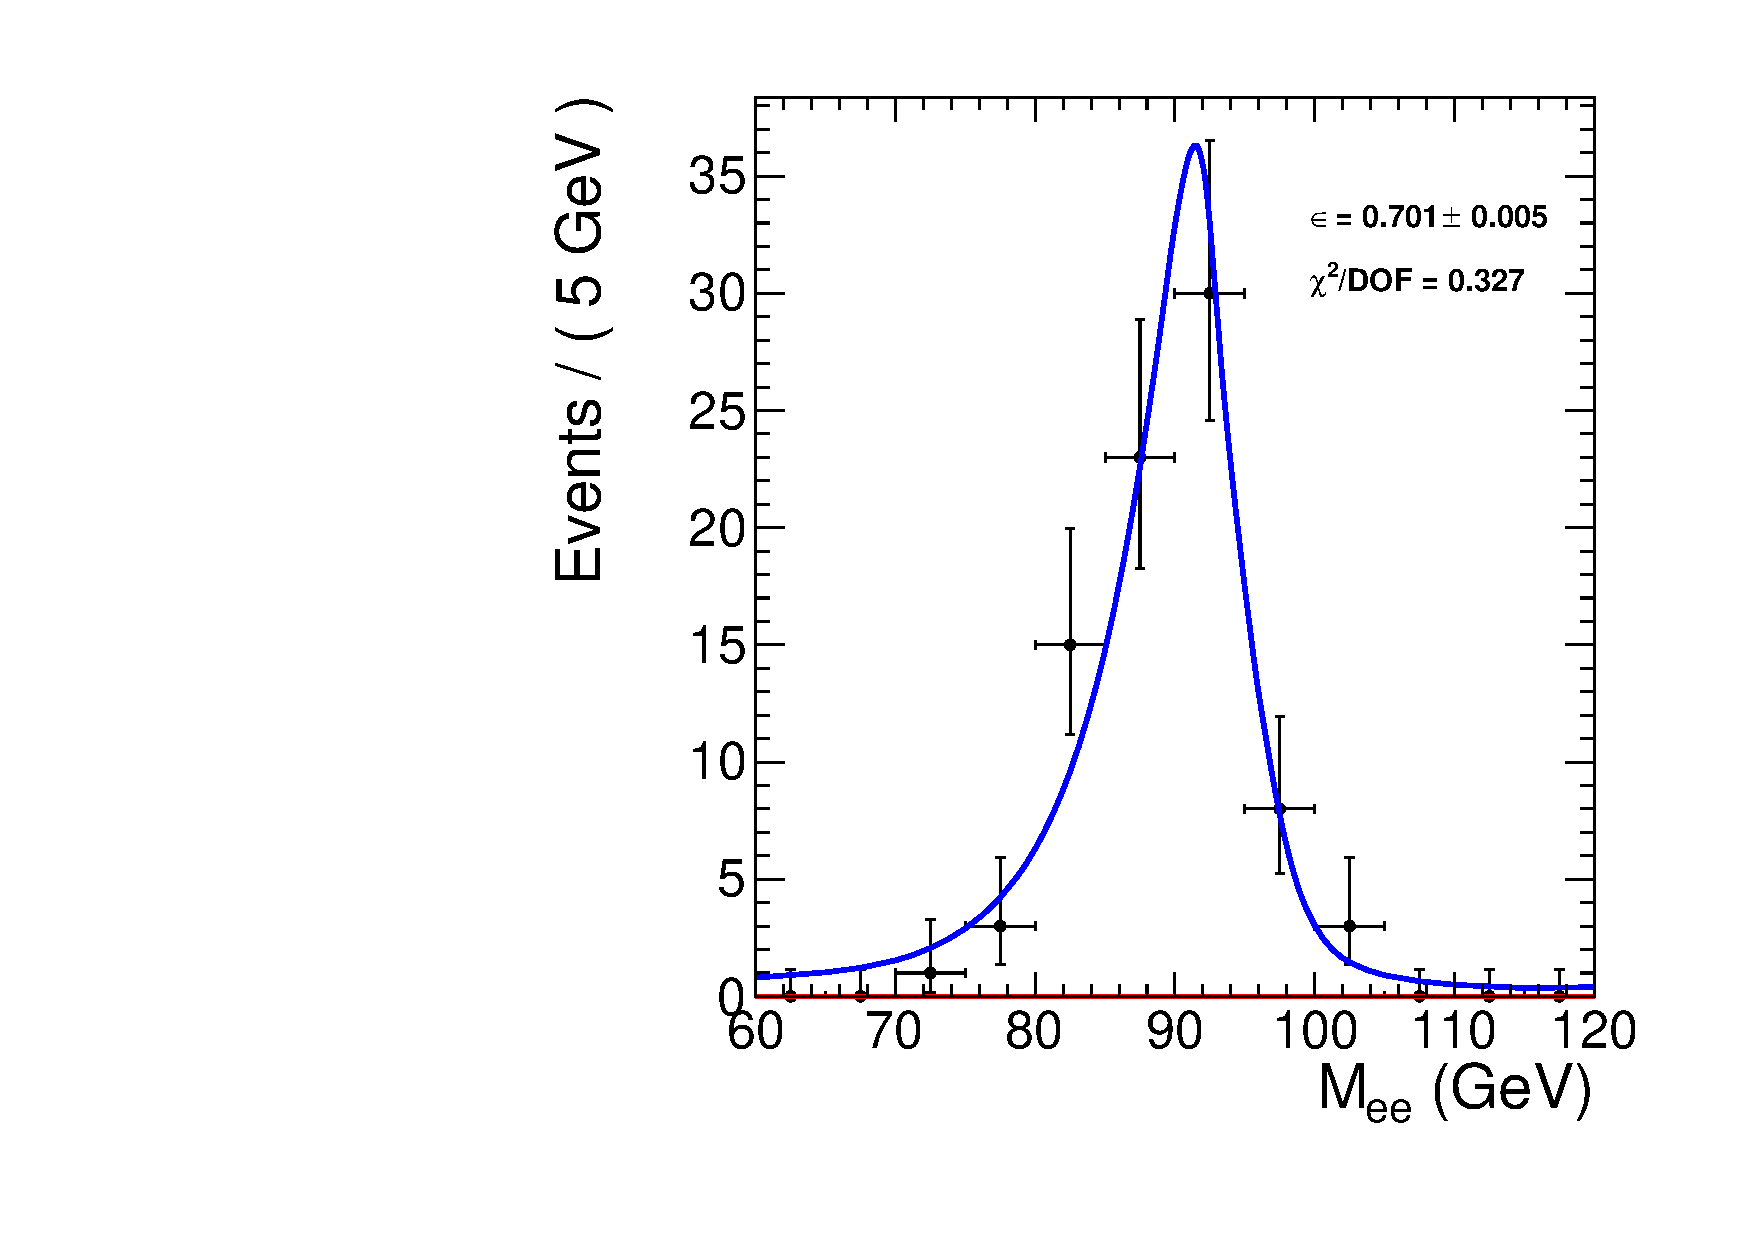
\includegraphics[width=0.49\textwidth]{tpHistos_ID80_ee_plus_fail.pdf}}
    \caption{The passing (a) and failing (b) fits for the Reco$\to$WP80 step in the Ecal Endcap for positrons.
             The data is in black, background fit in red, and signal+background fit in blue.}
  \end{center}
\end{figure}

\clearpage

%wp80->hlt
\begin{figure}[htb]
  \begin{center}
    \subfigure[]{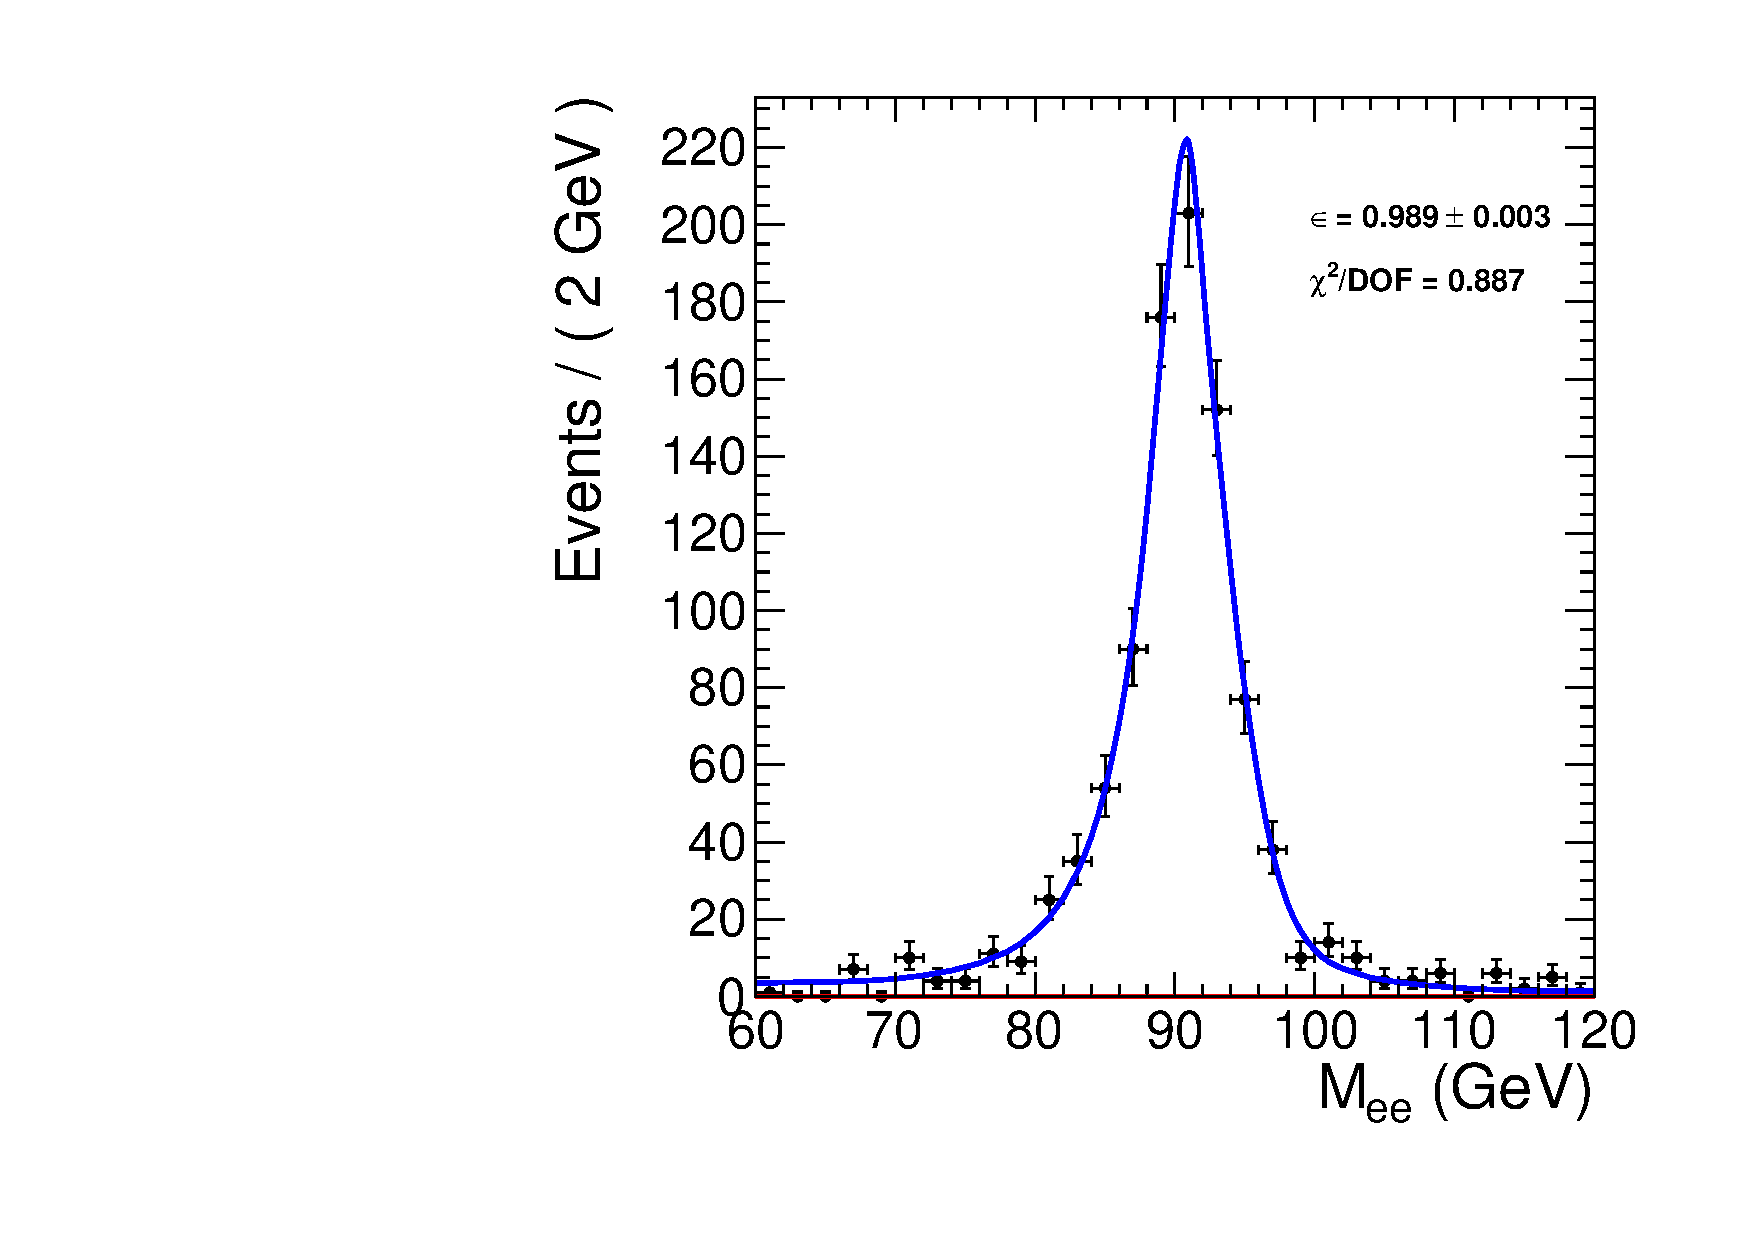
\includegraphics[width=0.49\textwidth]{tpHistos_HLT80_eb_pass.pdf}}
    \subfigure[]{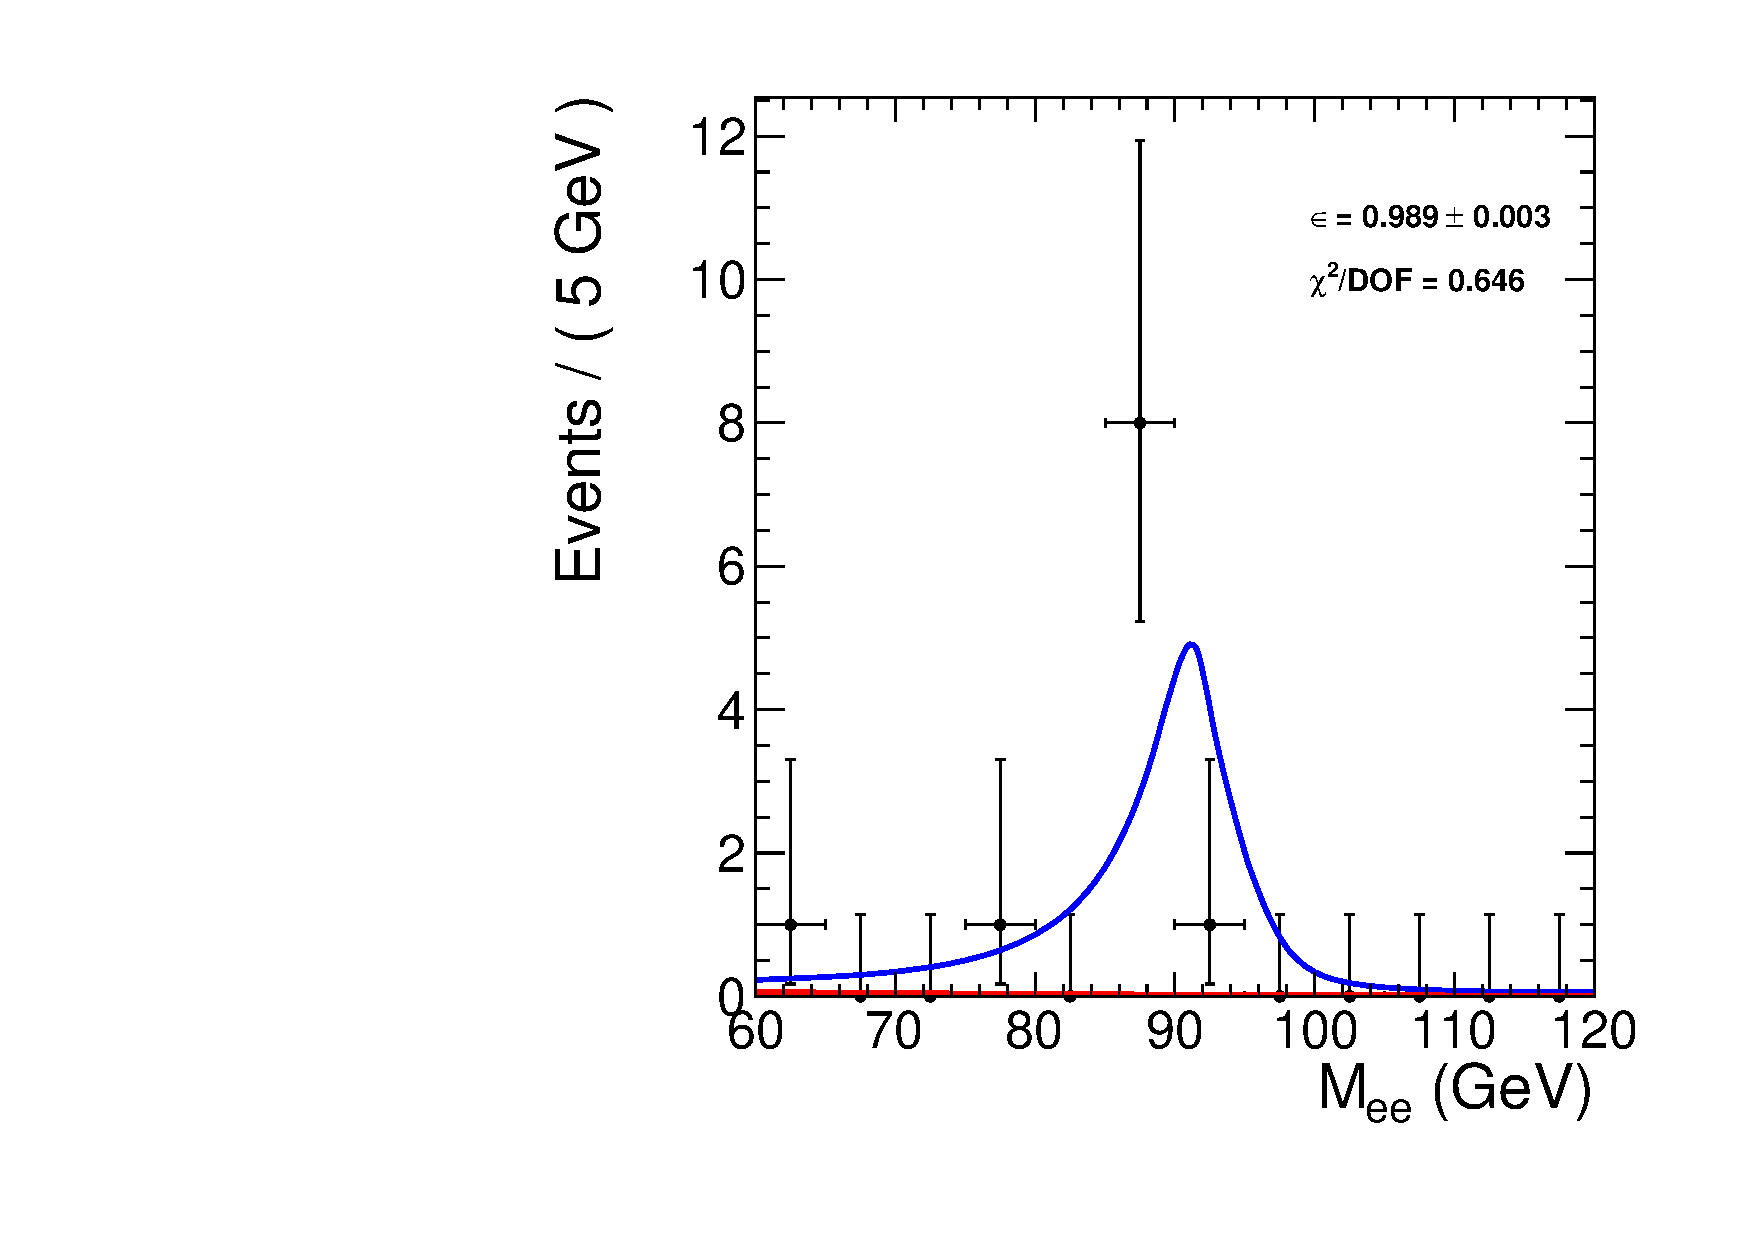
\includegraphics[width=0.49\textwidth]{tpHistos_HLT80_eb_fail.pdf}}
    \caption{The passing (a) and failing (b) fits for the WP80$\to$HLT step in the Ecal Barrel.
             The data is in black, background fit in red, and signal+background fit in blue.}
  \end{center}
\end{figure}

\begin{figure}[htb]
  \begin{center}
    \subfigure[]{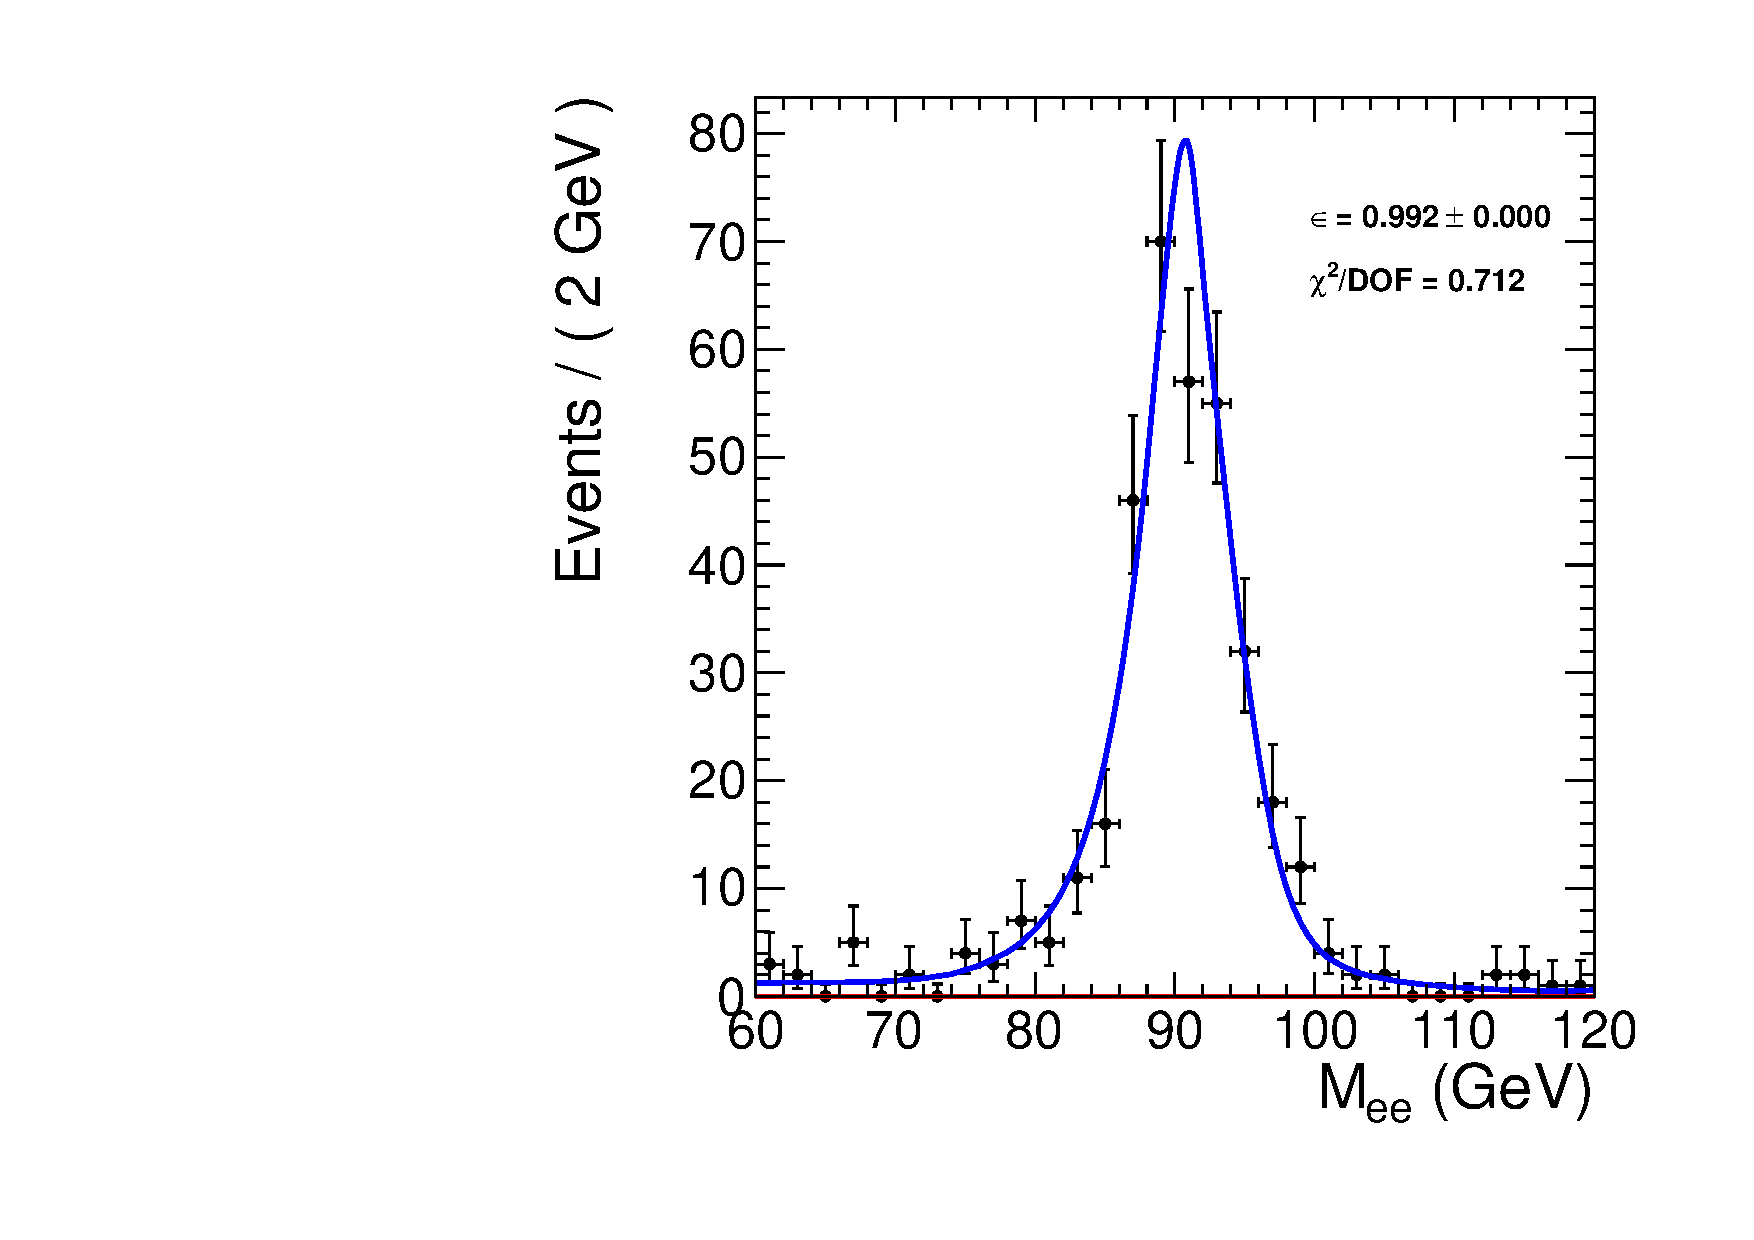
\includegraphics[width=0.49\textwidth]{tpHistos_HLT80_ee_pass.pdf}}
    \subfigure[]{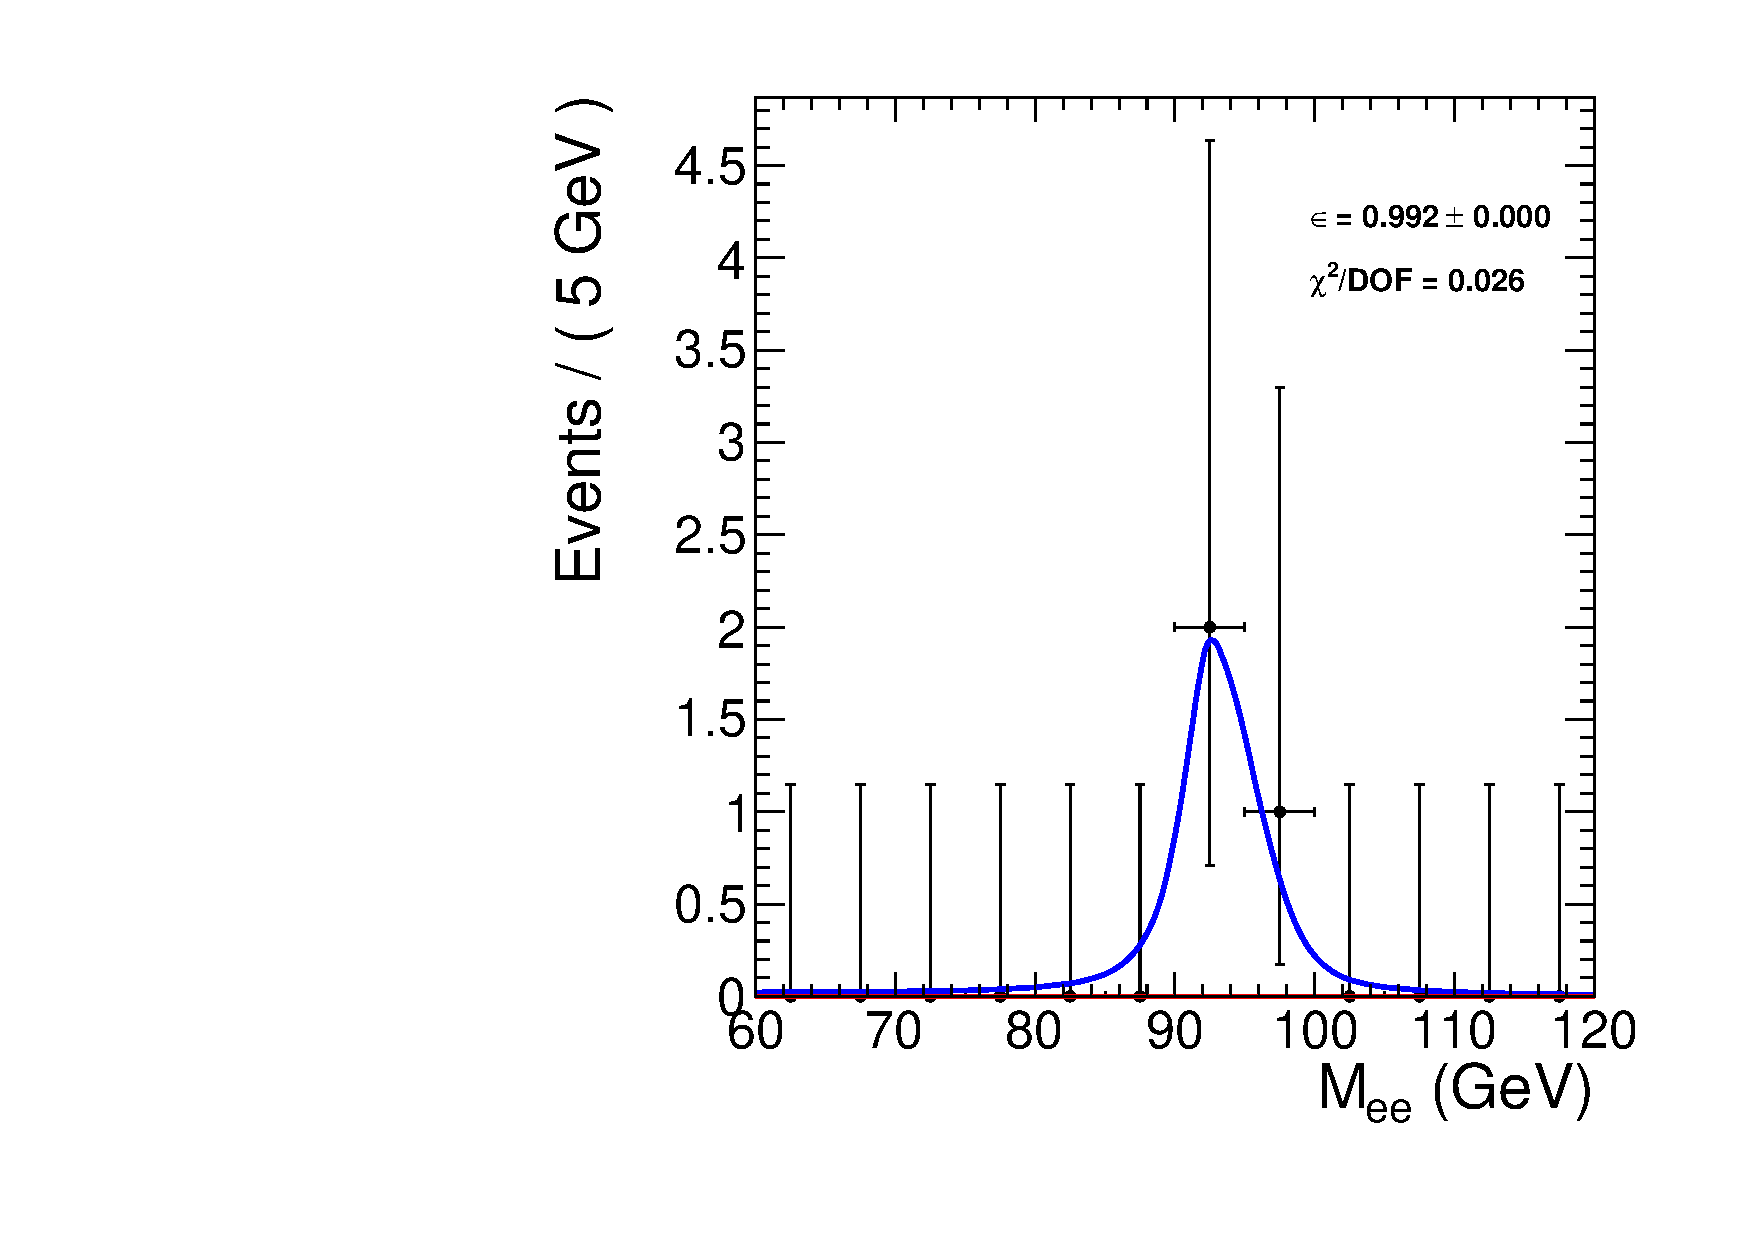
\includegraphics[width=0.49\textwidth]{tpHistos_HLT80_ee_fail.pdf}}
    \caption{The passing (a) and failing (b) fits for the WP80$\to$HLT step in the Ecal Endcap.
             The data is in black, background fit in red, and signal+background fit in blue.}
  \end{center}
\end{figure}

\begin{figure}[htb]
  \begin{center}
    \subfigure[]{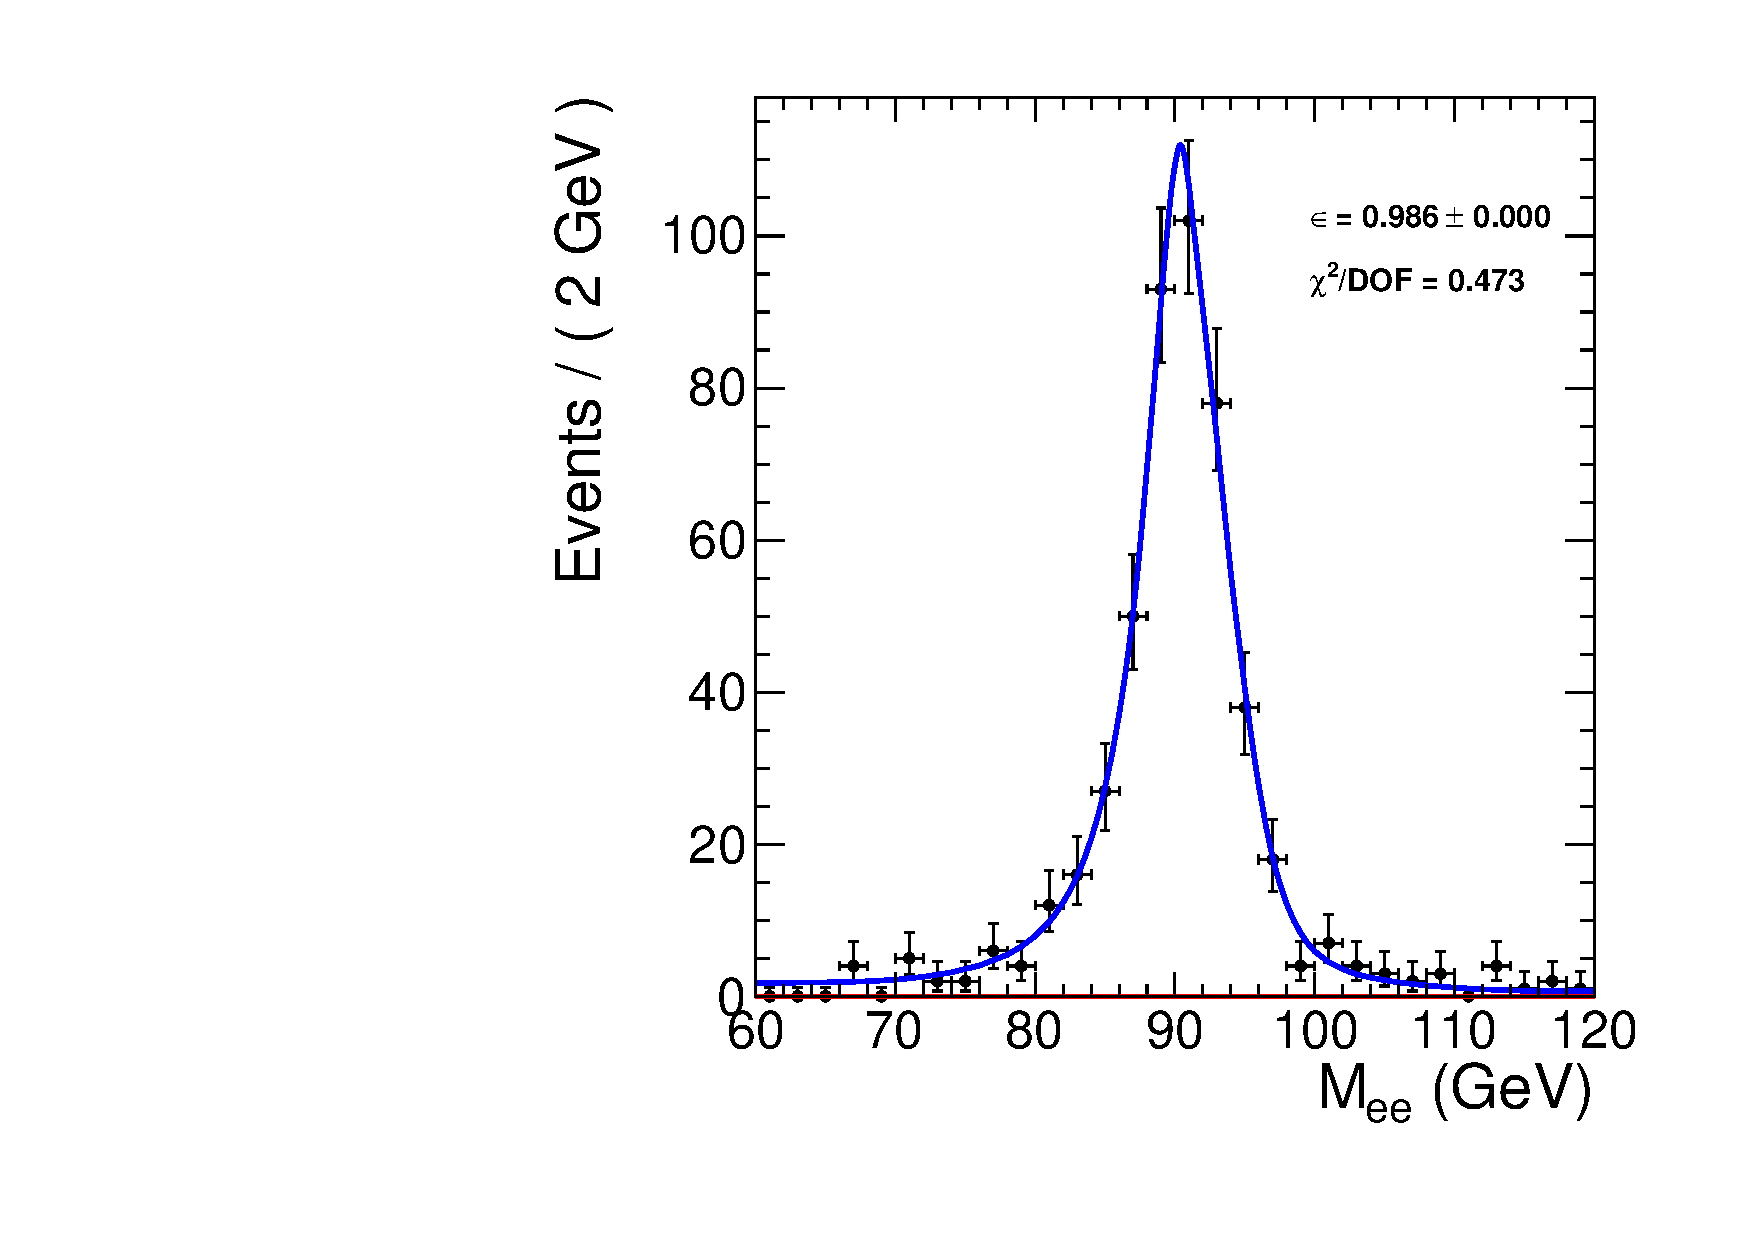
\includegraphics[width=0.49\textwidth]{tpHistos_HLT80_eb_minus_pass.pdf}}
    \subfigure[]{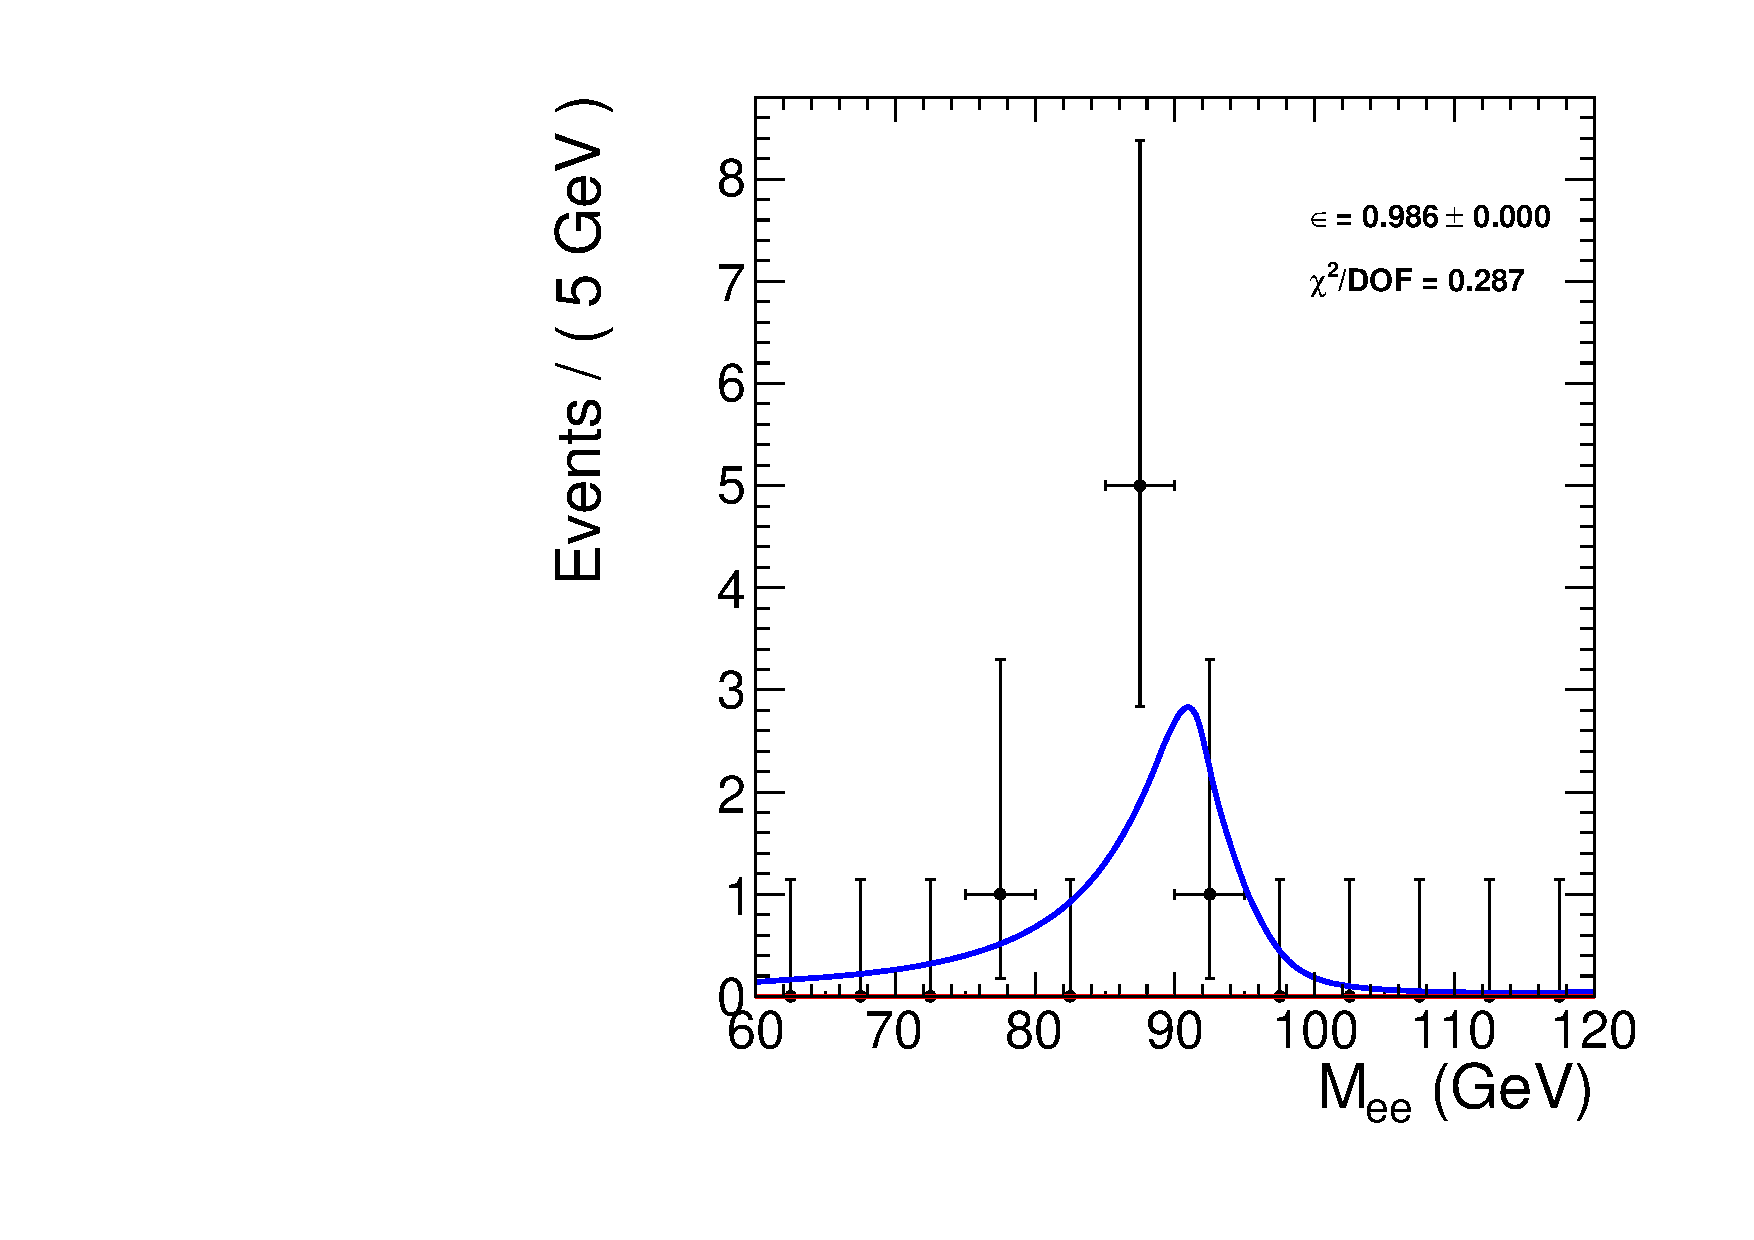
\includegraphics[width=0.49\textwidth]{tpHistos_HLT80_eb_minus_fail.pdf}}
    \caption{The passing (a) and failing (b) fits for the WP80$\to$HLT step in the Ecal Barrel for electrons.
             The data is in black, background fit in red, and signal+background fit in blue.}
  \end{center}
\end{figure}

\begin{figure}[htb]
  \begin{center}
    \subfigure[]{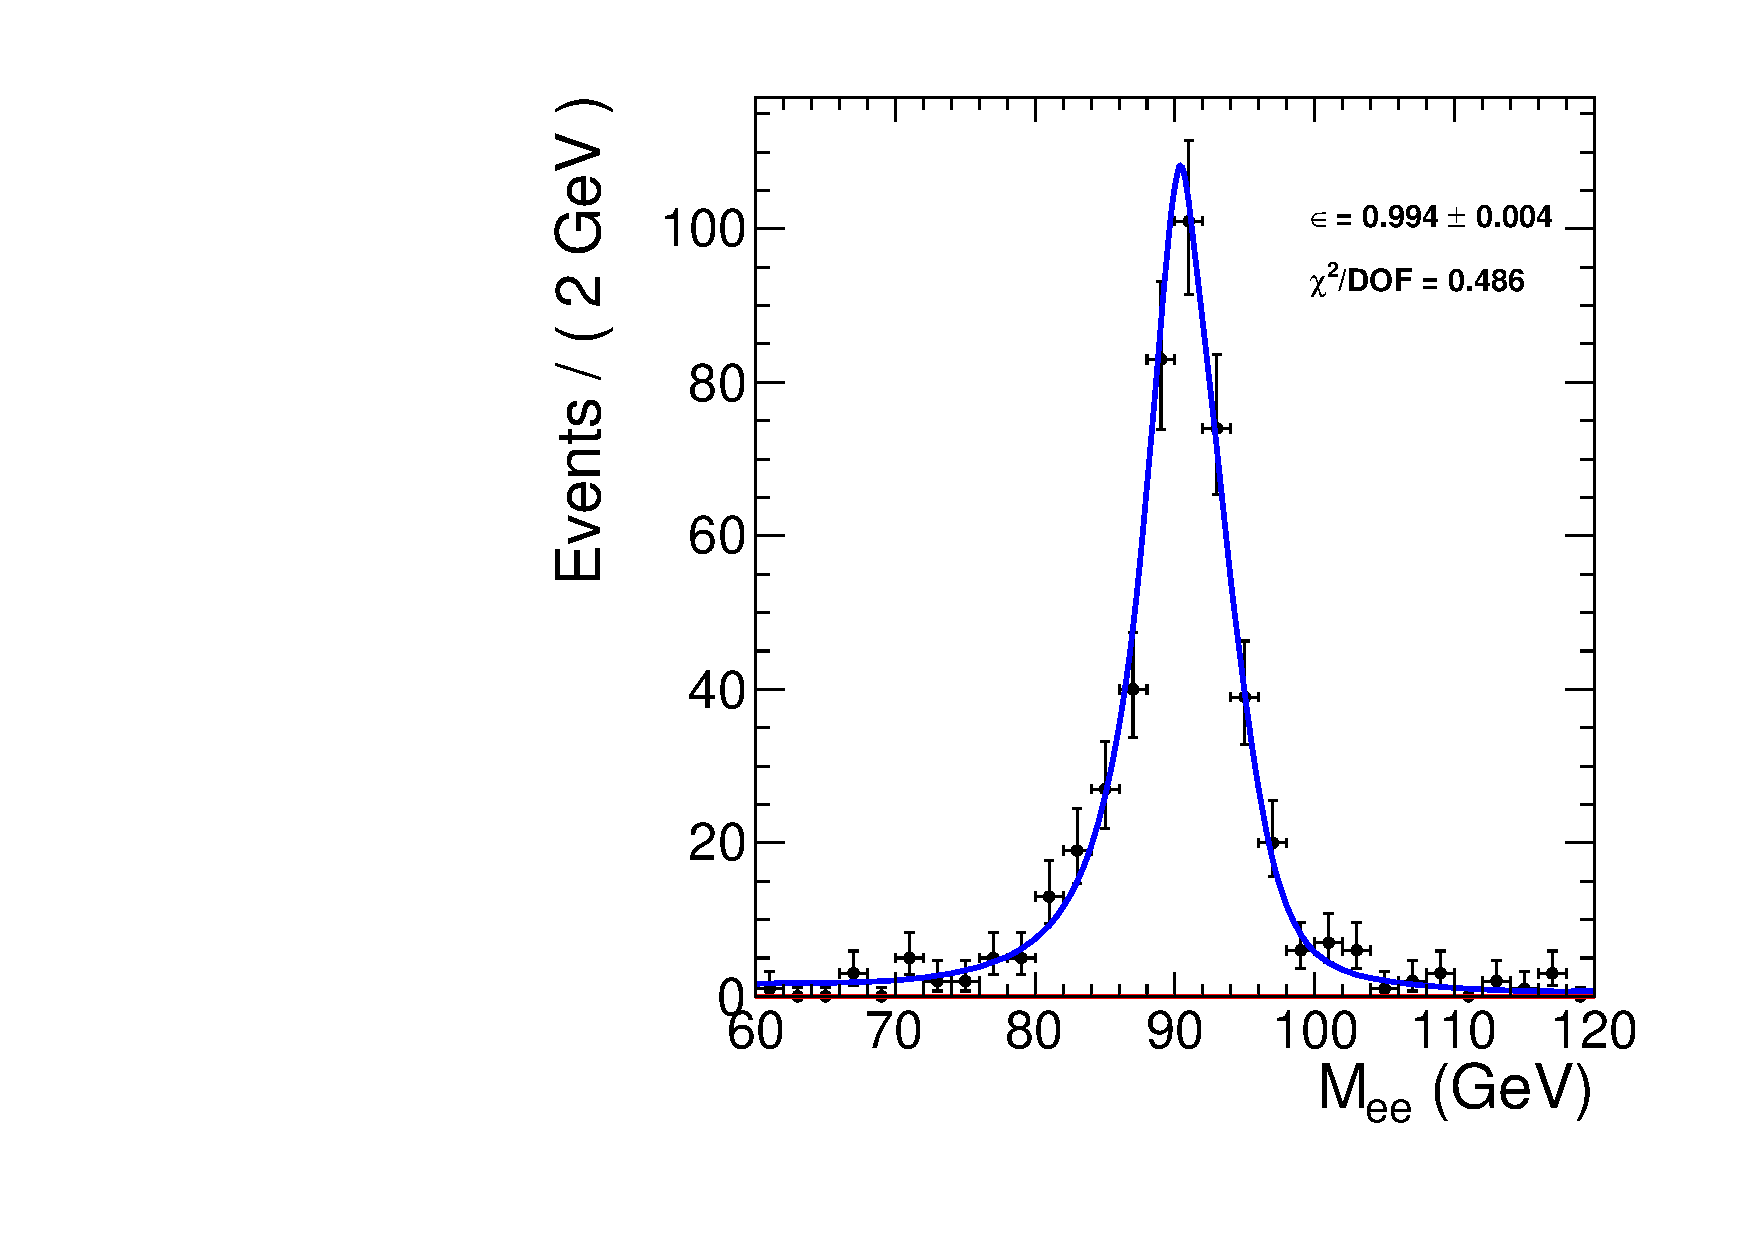
\includegraphics[width=0.49\textwidth]{tpHistos_HLT80_eb_plus_pass.pdf}}
    \subfigure[]{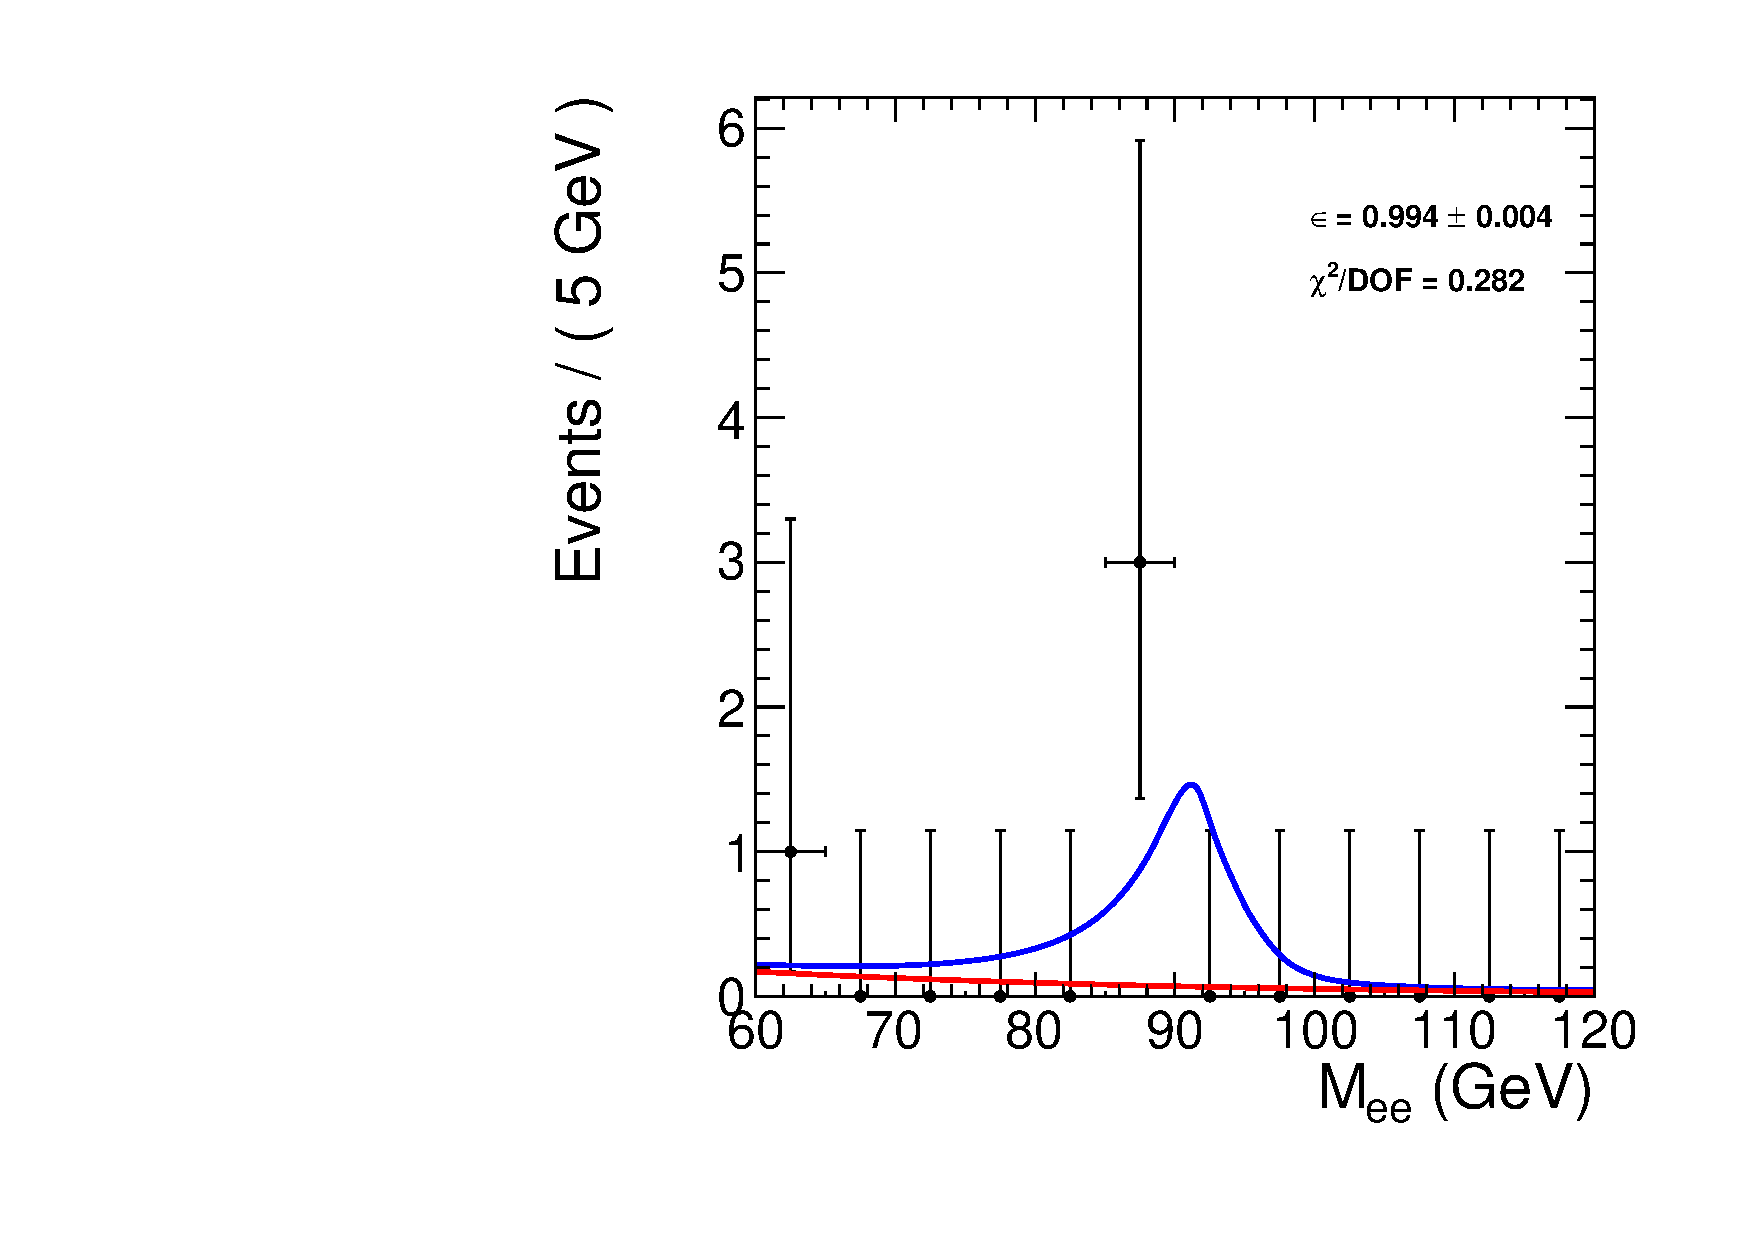
\includegraphics[width=0.49\textwidth]{tpHistos_HLT80_eb_plus_fail.pdf}}
    \caption{The passing (a) and failing (b) fits for the WP80$\to$HLT step in the Ecal Barrel for positrons.
             The data is in black, background fit in red, and signal+background fit in blue.}
  \end{center}
\end{figure}

\begin{figure}[htb]
  \begin{center}
    \subfigure[]{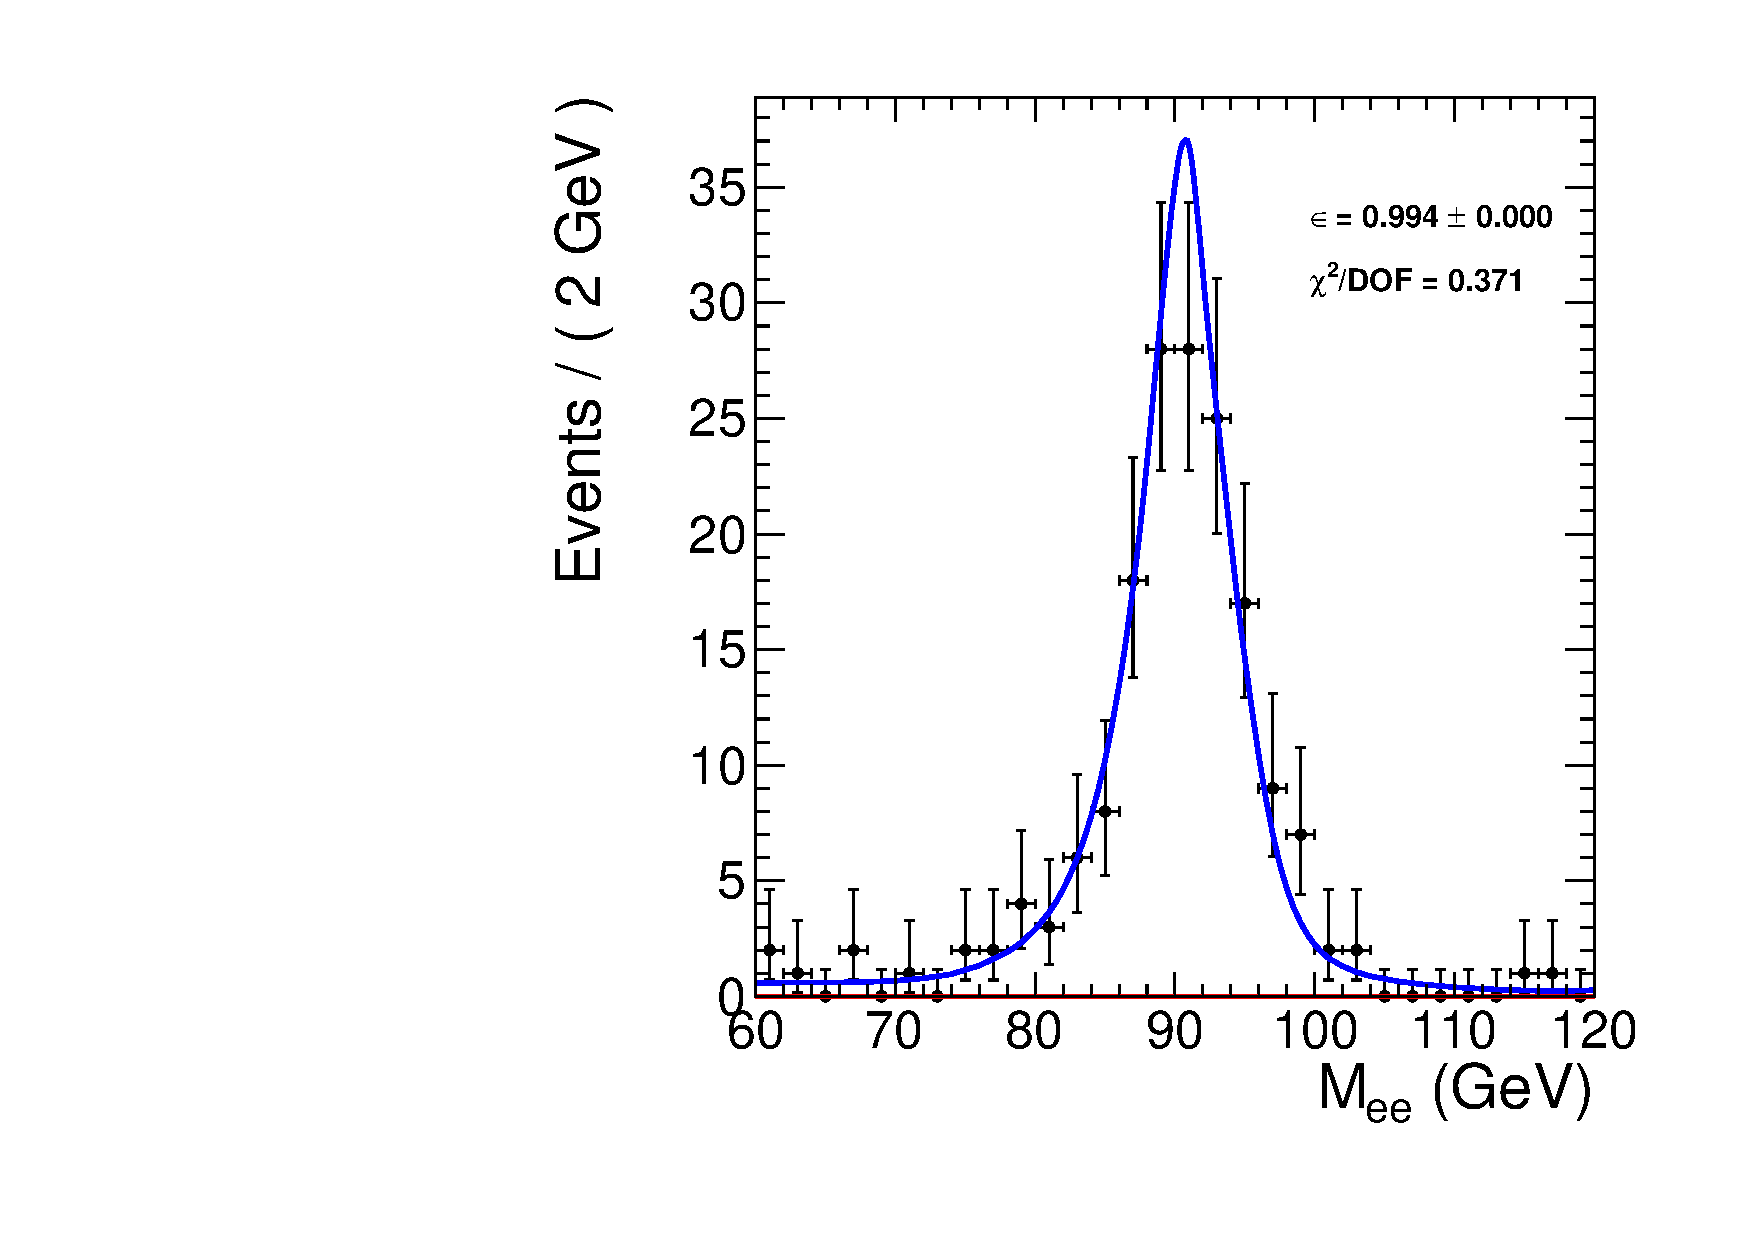
\includegraphics[width=0.49\textwidth]{tpHistos_HLT80_ee_minus_pass.pdf}}
    \subfigure[]{\includegraphics[width=0.49\textwidth]{tpHistos_HLT80_ee_minus_fail.pdf}}
    \caption{The passing (a) and failing (b) fits for the WP80$\to$HLT step in the Ecal Endcap for electrons.
             The data is in black, background fit in red, and signal+background fit in blue.}
  \end{center}
\end{figure}

\begin{figure}[htb]
  \begin{center}
    \subfigure[]{\includegraphics[width=0.49\textwidth]{tpHistos_HLT80_eb_plus_pass.pdf}}
    \subfigure[]{\includegraphics[width=0.49\textwidth]{tpHistos_HLT80_eb_plus_fail.pdf}}
    \caption{The passing (a) and failing (b) fits for the WP80$\to$HLT step in the Ecal Endcap for positrons.
             The data is in black, background fit in red, and signal+background fit in blue.}
  \end{center}
\end{figure}

\newpage

\end{thebibliography}
%\end{document}
